



\documentclass[12pt, a4paper]{report}






%-----------USEPACKAGE----------------------------
\usepackage{bm} % Tucne pismo
\usepackage[czech]{babel} % Cestina
\usepackage[T1]{fontenc}
\usepackage[utf8x]{inputenc}
\usepackage[unicode]{hyperref} % Odkazy v pdf, www a na e-mail
\usepackage{graphicx} % Obrazky
\usepackage{epstopdf} % Obrazky
\linespread{1.10} % Radkovani 1.3 odpovida radkovani 2
\usepackage{lmodern} % Daji se pouzit \HUGE atd.
\usepackage{amsmath}
\usepackage{algorithm}
\usepackage[noend]{algpseudocode} % Vkladani pseudo kodu

\usepackage[numbered,framed]{matlab-prettifier} %vkladani kodu matlabu
\lstset{style = Matlab-editor, basicstyle = \mlttfamily, escapechar = ", mlshowsectionrules = true,}








%------------------DRAFT----------------------------
\usepackage{draftwatermark}
\SetWatermarkLightness{0.95}
\SetWatermarkScale{1}
\SetWatermarkText{DRAFT}









%------------------LAYOUT----------------------------
\usepackage[top = 2.5 cm, bottom = 2.5 cm, left = 2.5 cm, right = 2.5 cm]{geometry} % geometrie stranky
\usepackage{longtable}% Pro dlouhy obsah, da se zalomit \pagebrek
\usepackage{fancyhdr}
\pagestyle{fancy}% Deffaultni nastaveni hlavicky a paticky
\setlength{\headheight}{16 pt}% Zvetsi hlavicku, aby to nedelalo warningy
\fancyhf{}
\lhead{\href{http://www.kky.zcu.cz/cs/courses/mpv}{Metody Počítačového Vidění}}
\rhead{8. přednáška}
\fancyfoot[R]{\thepage}
\fancyfoot[L]{Verze 1.0.0, poslední úpravy: \today}








\begin{document}











%--------TITULNI-STRANA------------------------------
\begin{titlepage}
\begin{center}
	
\includegraphics[trim = 0.6cm 0.5cm 0.9cm 0.5cm, scale=1]{./Img/FAV_logo_cz.pdf}
	\hspace*{\fill}
	
\includegraphics[trim = 3.5cm 1.5cm 2.6cm 2cm, scale=0.295]{./Img/KKY_logo_cz.pdf}\\
	\vspace*{\fill}
	\textbf{\Huge{\href{http://www.kky.zcu.cz/cs/courses/mpv}{Metody Počítačového Vidění} \\ 8. přednáška: Strojové učení}}\\
	\vspace*{\fill}
	\textbf{\large{\href{mailto:LBures@kky.zcu.cz}{Ing. Lukáš Bureš}}} \hfill ~\\
	\textbf{\large{\href{mailto:PetrZim@kky.zcu.cz}{Ing. Petr Zimmermann}}} \hfill \textbf{\large{Plzeň}}\\
	\textbf{\large{Katedra kybernetiky}} \hfill \textbf{\large{\today}}
\end{center}
\end{titlepage}










%--------OBSAH----------------------------------------
\setcounter{page}{1}
\pagenumbering{Roman}

\tableofcontents
\newpage

\setcounter{page}{1}
\pagenumbering{arabic}









%--------SEKCE----------------------------------------



%
%\chapter{TODO}
%
%\par{ \textbf{Tuně psané si vezme na starost Lukáš.}}
%
%\begin{itemize}
%	\item \par{Motivace - proč klasifikovat, co je to klasifikace, pojem experta,}
%	
%	\item \par{\textbf{Příznakový vektor - co to je, jak se sestavuje, (nevím jestli hovořit o volbě počtu příznaků a tím pádem o redukci příznaků, dále neví zda zmiňovat, že vektor nemusí obsahovat pouze reálná čísla}}
%	
%	\item \par{Učení s učitelem a \textbf{bez učitele(Volba počtu tříd)}}
%	
%	\item \par{Porovnávání vektorů II - na základě pravděpodobnostního rozdělení trénovací množiny, lineární/nelineární dělící rovina }
%	
%	\item \par{ \textbf{Ověření výsledku klasifikace - recall, precision, F1 skore}}
%\end{itemize}
%
%
%Update: 14. srpna 2014  
%\begin{itemize}
%	\item rozhodovaci les - co ta reference ?
%	\item Odstraneny jednopismenkove spojky z koncu radek v kapitole \ref{sec:DecisionTree}-\ref{sec:DecisionWald}
%	\item odstraněny warningy
%\end{itemize}
%
%Update: 28. srpna 2014
%\begin{itemize}
%	\item Dodelany reference od Lukase
%	\item Opraveny Petrovo uvozovky "" na \emph{\uv{}}
%\end{itemize}
%
%Update: 9.9.2014
%\begin{itemize}
%	\item Lukáš: Bayese, Bez ucitele - Kmeans, mean-shift, aglomerativni, divizni, (two threshold ?)
%	\item Petr:  Neuronovky, NN, KNN, Bayesuv nejak inteligentne - ne moc do hloubky, Perceptron
%	\item Motivace - koho napadne nejakz blaf, tak to tam napise.
%\end{itemize}
%
%
%



%-------PREDNASKA-08-------------------------------------------------------------------
%-LUKAS-BURES-&-PETR-ZIMMERMANN-
\chapter{Metody Počítačového Vidění: 8.~přednáška}
\label{sec:07}









%-------PRINCIP-KLASIFIKACE---------------------------------------------------------------
\section{Princip klasifikace}
\label{sec:07_Princip_Klasifikace}

\par{Ve strojovém učení a statistice je klasifikace problém identifikace, ke kterému ze souboru kategorií patří nová pozorování a to na základě trénovací množiny dat. Příkladem by mohl být antispamový filtr, který na základě jména klasifikuje do složek \uv{je spam} nebo \uv{není spam}.}

\par{V terminologii strojového učení je klasifikace za instanci učení s učitelem, tj učení, kde je k dispozici trénovací sada správně označených pozorování. Podobně, klasifikaci, kde není informace od učitele se říká shlukování a zahrnuje seskupování dat do kategorií na základě jisté míry přirozené podobnosti nebo vzdálenosti.}

\par{Často mají jednotlivá pozorování sadu měřitelných vlastností. Tyto vlastnosti mohou představovat jednotlivé kategorie například typ krevní skupiny, pořadové číslo (\uv{malé}, \uv{střední}, \uv{velké}.}

\par{Algoritmus, který provádí klasifikaci a to zejména v konkrétním provedení je známý jako klasifikátor. Termín \uv{klasifikátor} někdy také odkazuje na matematické funkce, realizované klasifikačním algoritmem, který mapuje vstupní data do kategorií.}

\par{Terminologie skrze vědecké oblasti je velice pestrá. Ve statistice, kde se klasifikace často provádí binární regresí nebo obdobným postupem se pozorované proměnné nazývají \uv{nezávislé proměnné} a predikované kategorie jsou známé jako výsledky, které je možné považovat za závislé proměnné. Ve strojovém učení jsou pozorování známá jako instance a nezávislé proměnné jsou nazývány příznaky, které se sdružují do příznakových vektorů. Dále jsou kategorie nazývány třídami.}

\newpage






\subsection{Porovnání příznakových vektorů}
\par{Jednotlivé příznakové vektory mohou být chápány jako body v mnohodimenzionálním prostoru a~úkolem klasifikace (klasifikátoru) je rozdělení tohoto prostoru na podprostory představující klasifikační třídy $\omega_{1,\ldots,N}$. Cílem je tedy rozdělit množinu příznakových vektorů $X$ na podmnožiny, tak aby platila následující podmínka
\begin{eqnarray}
	\nonumber
	&\omega_{1,\ldots,N} &\subset X,\\
	\nonumber
	&\bigcup_{i=1}^N &= X,\\
	\nonumber
	&\omega_i \cap \omega_j &= \emptyset, \textrm{pro }~i,j=1,\ldots,N,~\textrm{ }~i\neq j,
\end{eqnarray}}

\par{Třídy (shluky) v sobě sdružují vektory, které jsou si navzájem podobné (viz Obr.~\ref{fig:porov01}~). Podobnost vektorů je subjektivní pojem a výsledek klasifikace tak musí být ověřen expertem, který rozhodne, zda je výsledek klasifikace přípustný. Obecně platí, že pokud je vhodně sestaven příznakový vektor, lze vektory rozřazovat do shluků na základě tzv. míry podobnosti či odlišnosti.
\begin{figure}[!ht]
	\centering
	%trim option's parameter order: left bottom right top
	%\fbox{
	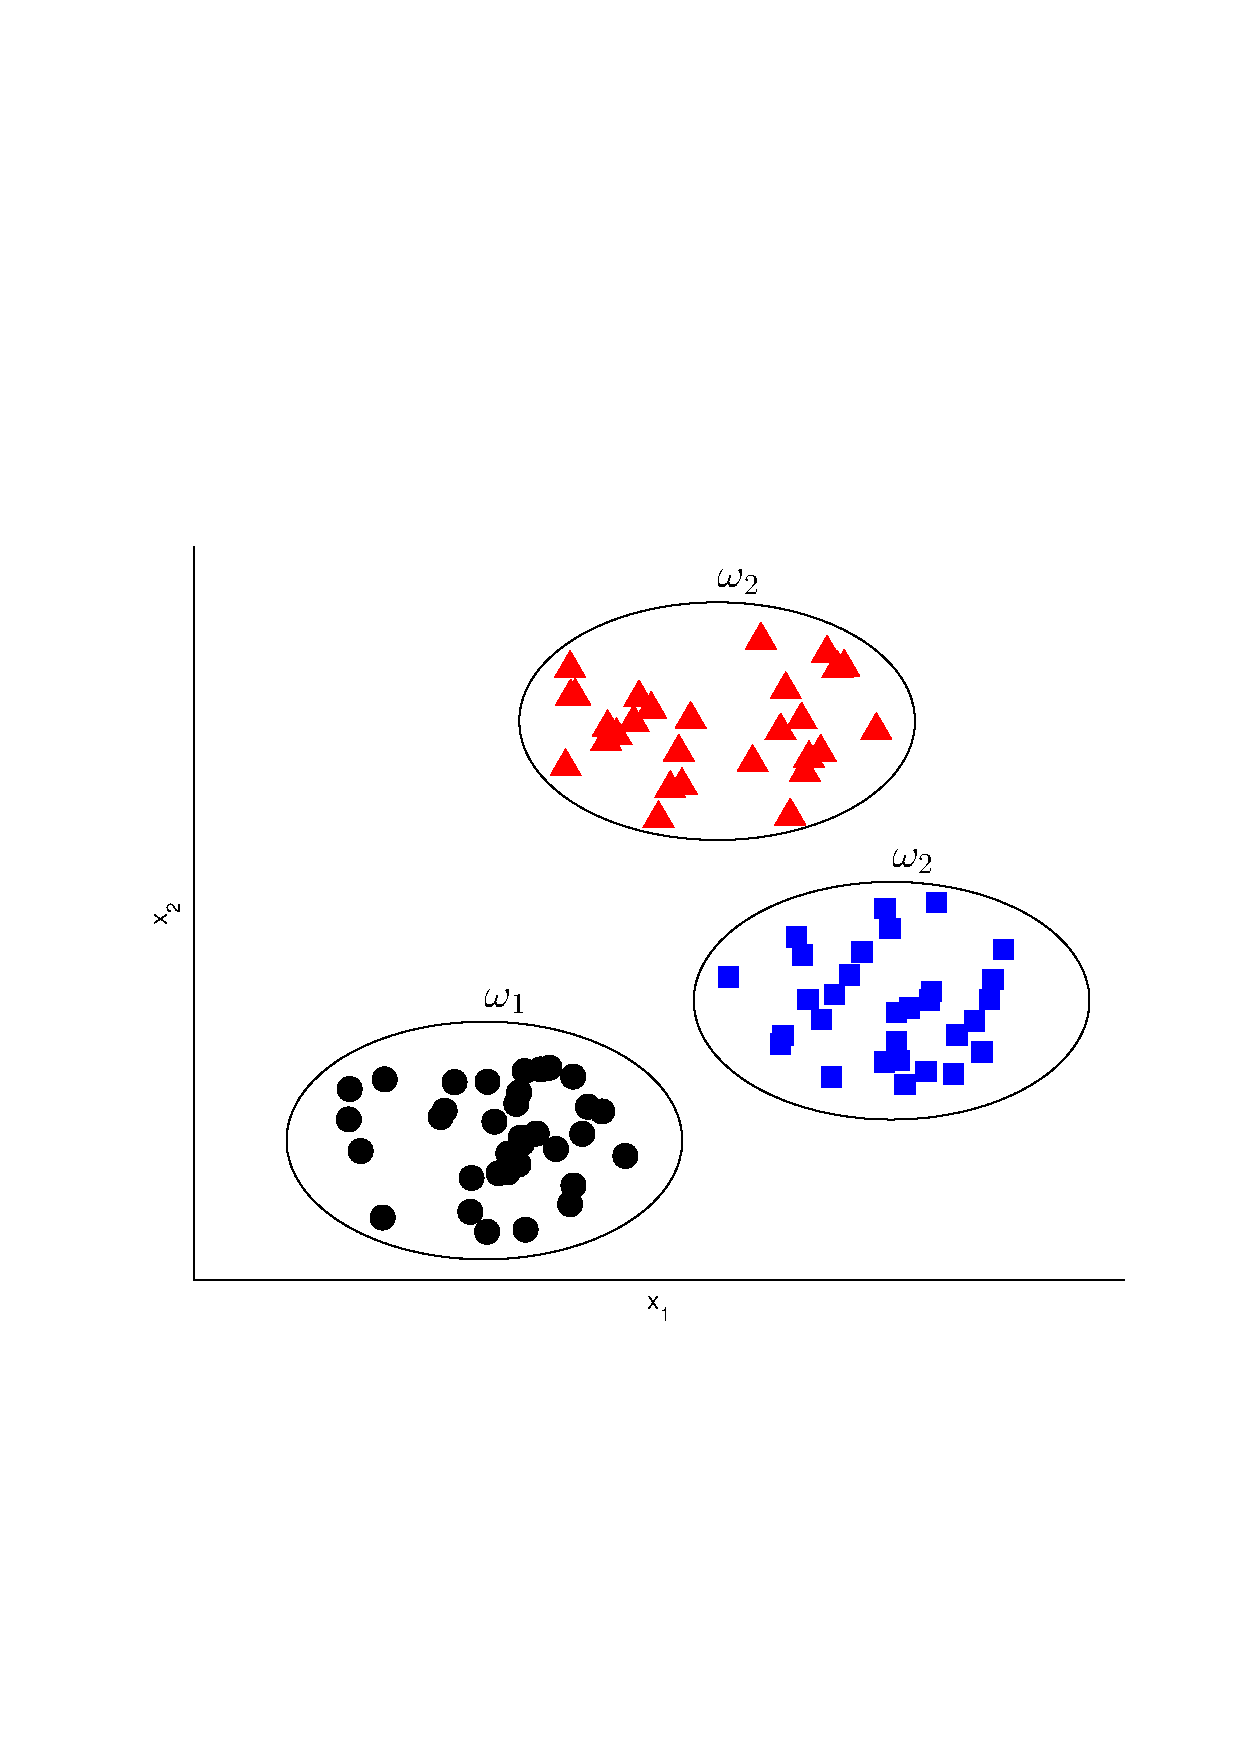
\includegraphics[width = 0.6\textwidth, trim = 3cm 7.5cm 2cm 9cm]{./Img/Prednaska08/Porovnani/porov01.pdf}
	\caption{Klasifikace do tří tříd.}
	\label{fig:porov01}
\end{figure}}

\par{Obě míry interpretují vzdálenost dvou vektorů v prostoru. Liší se pouze tím, že míra podobnosti pro dva stejné vektory dosahuje maximálních hodnot, naopak míra odlišnosti je pro takové vektory minimální.}

\newpage










\subsection{Míra podobnosti}
\par{Míra podobnosti $s$ dvou vektorů z množiny $X$ je definována jako
\begin{equation}	
	{s:X \times X \longrightarrow \mathcal{R},}
\end{equation}
kde $\mathcal{R}$ je množina reálných čísel, tak že
\begin{eqnarray}
	\exists s_0 \in \mathcal{R}:-\infty < s \left( \bm{x},\bm{y} \right) \geq s_0 < +\infty , &\quad \forall \bm{x},\bm{y}\in X,\\
	%
	s \left( \bm{x},\bm{y} \right)=s \left( \bm{y},\bm{x} \right), &\quad \forall \bm{x},\bm{y}\in X,\\
	%
	s \left( \bm{x},\bm{x} \right)=s_0, &\quad \forall \bm{x}\in X.~~~~
\end{eqnarray}
V praxi nejpoužívanější míry podobnosti jsou:
\begin{itemize}
	\item Skalární součin
	\begin{equation}
		s_\text{\textit{skal.souč.}} \left( \bm{x}, \bm{y} \right) = \bm{x}^{\top} \bm{y} = \sum_{ i = 1}^{l} x_i y_i,
	\end{equation}
	kde $l$ je dimenze vektorů $\bm{x}$ a $\bm{y}$. Skalární součin je používán v případě, že jsou porovnávané vektory normalizované, což znamená, že mají stejnou délku. Míra $s_\text{\textit{skal.souč.}} \left( \bm{x}, \bm{y} \right)$ vyjadřuje úhel svíraný vektory $\bm{x}$ a $\bm{y}$.
	\item Kosinová podobnost
	\begin{equation}
		{s_{cos}\left(\bm{x},\bm{y}\right)=\frac{\bm{x}^{\top}\bm{y}}{\|\bm{x}\|\|\bm{y}\|},}
	\end{equation}
	kde $\|\bm{x}\|=\sqrt{\sum_{i=1}^lx_i^2}$ a $\|\bm{y}\|=\sqrt{\sum_{i=1}^ly_i^2}$ je délka vektoru $\bm{x}$, resp. $\bm{y}$.
	\item Tanimotova míra
	\begin{equation}
		{s_T\left(\bm{x},\bm{y}\right)=\frac{\bm{x}^{\top}\bm{y}}{\|\bm{x}\|^2+\|\bm{y}\|^2-\bm{x}^{\top}\bm{y}}.}
	\end{equation}
\end{itemize}}














\subsection{Míra odlišnosti}
\par{Míra podobnosti $d$ dvou vektorů z množiny $X$ je definována jako
\begin{equation}	
	{d:X \times X \longrightarrow \mathcal{R},}
\end{equation}
kde $\mathcal{R}$ je množina reálných čísel, tak že
\begin{eqnarray}
	\exists d_0 \in \mathcal{R}:-\infty \leq d_0 < d \left( \bm{x},\bm{y} \right) < +\infty , &\quad \forall \bm{x},\bm{y}\in X,\\
	%
	d \left( \bm{x},\bm{y} \right)=d \left( \bm{y},\bm{x} \right), & \quad \forall \bm{x},\bm{y}\in X,\\
	%
	d \left( \bm{x},\bm{x} \right) = d_0 , & \quad \forall \bm{x}\in X.~~~~
\end{eqnarray}
Mezi nejčastěji používané míry odlišnosti patří:
\begin{itemize}
	\item $l_p$-norma
	\begin{equation}
		{d_p\left(\bm{x},\bm{y}\right)=\left(\sum_{i=1}^l|x_i-y_i|^p\right)^\frac{1}{p}.}
	\end{equation}
	\item $l_1$-norma (tzv. norma Manhattan)
	\begin{equation}
		{d_1\left(\bm{x},\bm{y}\right)=\sum_{i=1}^l|x_i-y_i|.}
	\end{equation}
	\item $l_\infty$-norma
	\begin{equation}
		{d_\infty\left(\bm{x},\bm{y}\right)=\max_{1\leq i \leq l}|x_i-y_i|.}
	\end{equation}
\end{itemize}}

\par{Výše uvedené míry mají i tzv. vážené formy. Ty získáme doplněním koeficientu $w_i~\geq~0$ před jednotlivé absolutní hodnoty, koeficient pak vyjadřuje váhy příslušných prvků příznakového vektoru. Díky svému chování jsou míry odlišnosti často označovány jako vzdálenost dvou vektorů. Známá Euklidova vzdálenost je získána pouhou modifikací $l_p$-normy.}













\subsection{Porovnání vektoru a třídy}
\par{V mnoha klasifikačních algoritmech dochází k začlenění příznakového vektoru $\bm{x}$ do třídy $\omega$ na základě porovnání $\rho\left(\bm{x},\omega\right)$, přičemž porovnání $\rho$ může představovat jakoukoli míru podobnosti, resp. odlišnosti. V praxi se porovnání mezi vektorem a třídou provádí dvěma způsoby. V prvním jsou při stanovení $\rho\left(\bm{x},\omega\right)$ brány v potaz všechny vektory tvořící třídu $\omega$. Mezi typické představitele prvního způsobu porovnání vektoru a třídy patří:
\begin{itemize}
	\item Maximální podobnostní funkce
	\begin{equation}
		{\rho_{max}\left(\bm{x},\omega\right)=\max_{\bm{y}\in\omega}\rho\left(\bm{x},\bm{y}\right).}
	\end{equation}
	\item Minimální podobnostní funkce
	\begin{equation}
		{\rho_{min}\left(\bm{x},\omega\right)=\min_{\bm{y}\in\omega}\rho\left(\bm{x},\bm{y}\right).}
	\end{equation}
	\item Průměrná podobnostní funkce
	\begin{equation}
		{\rho_\text{\textit{prům.}}\left(\bm{x},\omega\right)=\frac{1}{n_\omega}\sum_{\bm{y}\in\omega}\rho\left(\bm{x},\bm{y}\right),}
	\end{equation}
	kde $n_\omega$ značí počet vektorů tvořících třídu $\omega$.
\end{itemize}}

\par{V druhém způsobu porovnání je třída zastoupena svým reprezentantem. Porovnání je v tomto případě stanoveno na základě vztahu $\rho\left(\bm{x},\omega_{rep}\right)$, přičemž $\omega_{rep}$ představuje vektor reprezentující třídu $\omega$. Je zřejmé, že za $\rho$ lze opět dosadit jakoukoli míru podobnosti či odlišnosti.}







\newpage






\subsection{Reprezentant třídy}
\par{Mezi typické volby reprezentanta třídy patří:
\begin{itemize}
	\item Průměr
	\begin{equation}
		{\bm{\omega}_p=\frac{1}{n_\omega}\sum_{\bm{y}\in\omega}\bm{y},}
	\end{equation}
	kde $n_\omega$ je počet prvků uvnitř třídy $\omega$. Průměr je nejčastější volbou reprezentanta třídy, jelikož je velice jednoduché ho stanovit. Nevýhodou ovšem je, že průměr nemusí být součástí třídy. Pokud usilujeme o to, aby reprezentant byl opravdu prvkem dané třídy je vhodnější zvolit střed či medián.
	\item Střed $\bm{\omega}_c\in\omega$ je vektor splňující:
	\begin{equation}	
		\sum_{ \bm{y} \in \omega} d \left( \bm{\omega}_c, bm{y} \right) \leq \sum_{\bm{y}\in\omega} d \left( \bm{z}, \bm{y} \right), \quad \forall \bm{z} \in \omega,
	\end{equation}
	kde $d$ značí míru odlišnosti (pokud by byla použita míra podobnosti $s$ je nutné v~předpisu otočit znaménka nerovnosti).
	\item Medián $\bm{\omega}_{med}\in\omega$ je vektor splňující:
	\begin{equation}
		med \left( d \left( \bm{\omega}_{med}, \bm{y} \right) | \bm{y} \in \omega \right) \leq med \left( d \left( \bm{z}, \bm{y} \right) | \bm{y} \in \omega \right), \quad \forall \bm{z} \in \omega,	
	\end{equation}
\end{itemize}
kde $d$ je míra odlišnosti.}

\par{Uvedené reprezentanty třídy lze použít pouze v případě, že je třída kompaktní (viz Obr. \ref{fig:porov02}). Pokud jsou prvky uvnitř třídy uspořádané lineárně či do kružnice (sféry) je vhodnější porovnávat vektory s těmito typy tříd na základě vzdálenosti od přímky (roviny), resp. kružnice (sféry).
\begin{figure}[!ht]
	\centering
	%trim option's parameter order: left bottom right top
	%\fbox{
	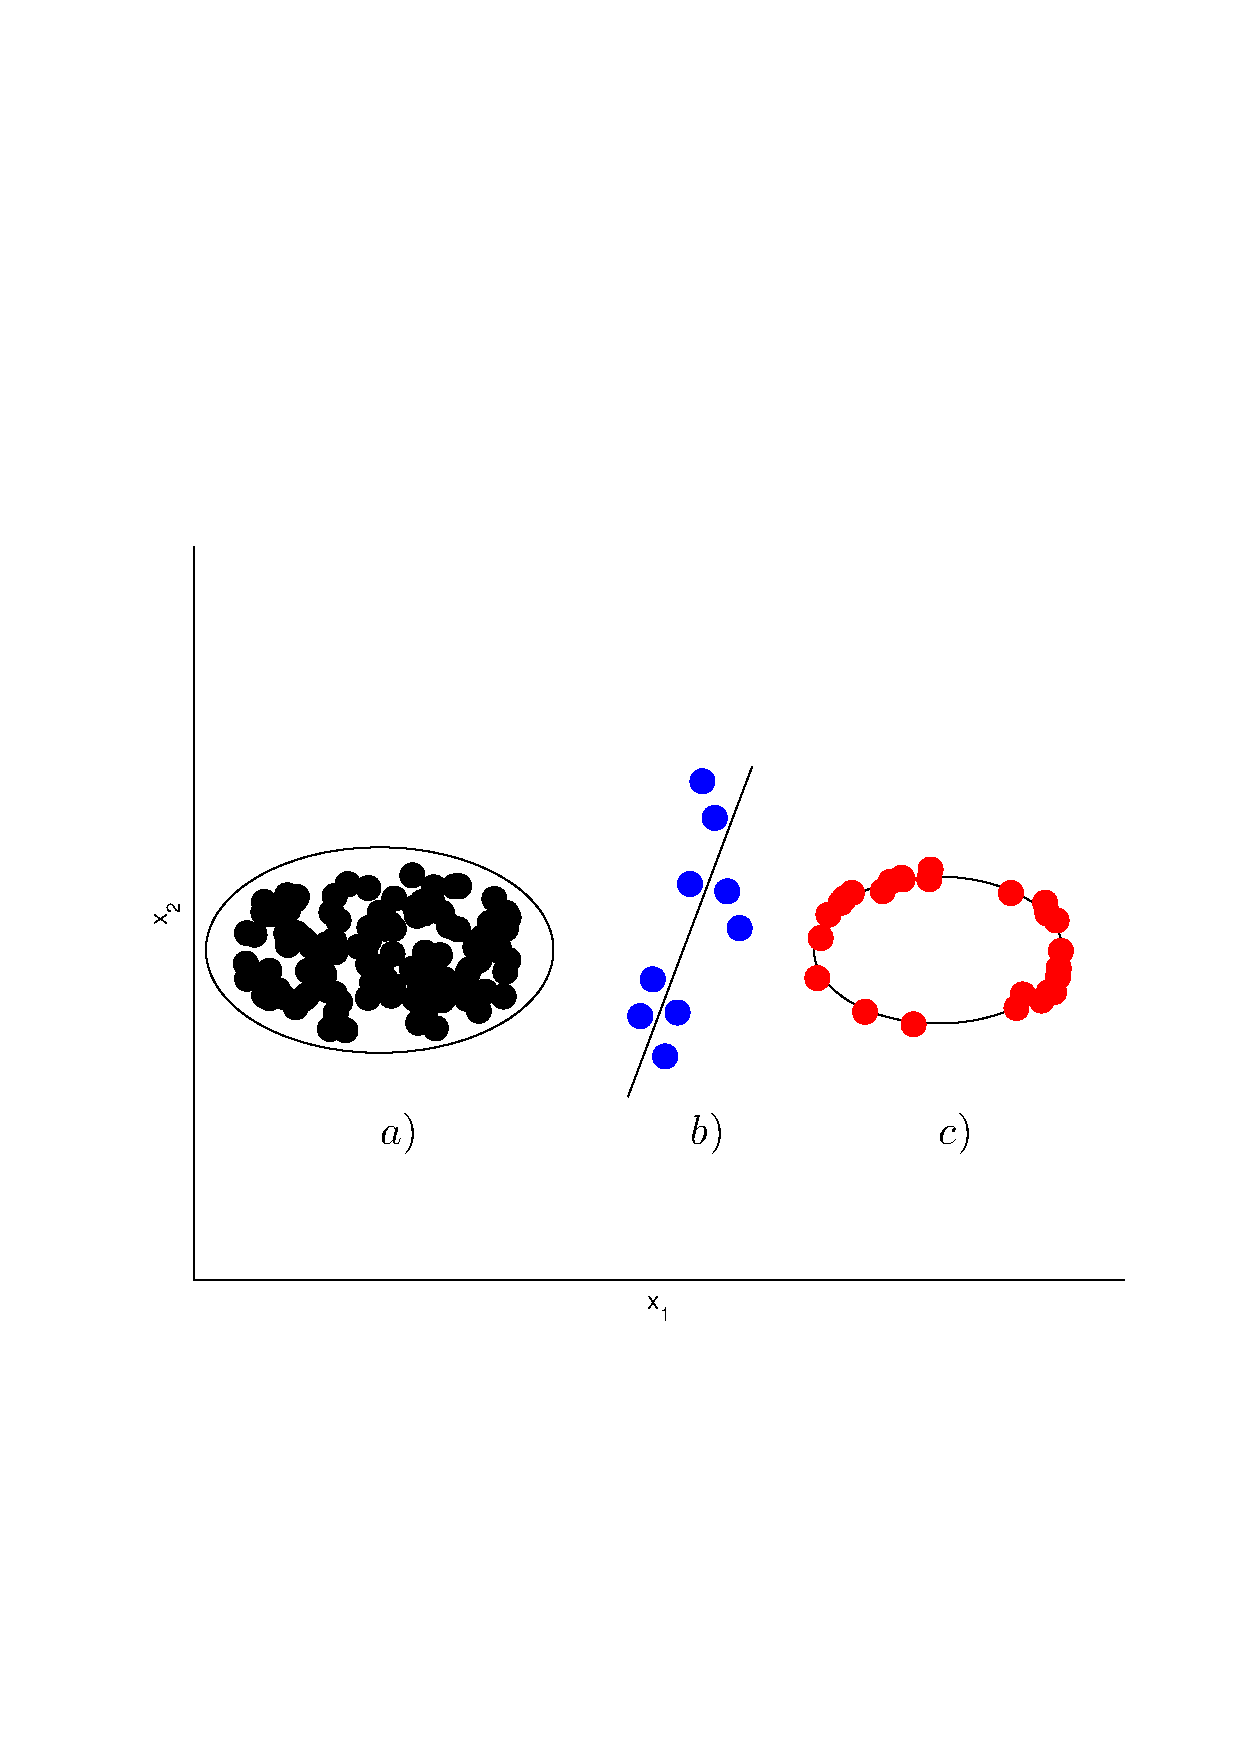
\includegraphics[width = 0.6\textwidth, trim = 3cm 7.5cm 2cm 9cm]{./Img/Prednaska08/Porovnani/porov02.pdf}
	\caption{Příklad třídy $a)$ kompaktní, $b)$ lineární a $c)$ sférické..}
	\label{fig:porov02}
\end{figure}}

\newpage
























%----CO-JE-STROJOVE-UCENI-------------------------------------------------------------------
\subsection{Co je strojové učení?}
\label{sec:UvodCoJeStrojoveUceni}

\par{Pojem strojové učení nemá dodnes pevně danou definici, můžeme si ukázat několik pokusů o jeho definování
\begin{itemize}
	\item Arthur Samuel (1959). Strojové učení: \textit{Obor, který dává počítačům schopnost učit se bez toho, aby byly přímo naprogramovány.}
	\item Tom Mitchell (1998): Dobře definovaný problém strojového učení: \textit{Předpokladem je, že se počítačový program učí ze zkušeností \textbf{E} s respektováním úlohy \textbf{T} a s měřičem výkonu \textbf{P}, pokud se jeho výkon na úloze \textbf{T} měřený pomocí \textbf{P} zvyšuje se zkušeností \textbf{E}.}
\end{itemize}}

\par{Pokusme se jednotlivé části rozebrat na příkladu: Předpokládejme, že náš emailový klient sleduje, které email označíme nebo neoznačíme jako spam. Na základě tohoto rozhodnutí se náš emailový klient učí lépe rozpoznávat co je a co není spam. Nyní si můžeme položit otázku co z následujících tvrzení je úloha \textbf{T}?
\begin{enumerate}
	\item Klasifikace emailů jako spam nebo vyžádaný email.
	\item Sledování značek od uživatele, který email označil jako spam nebo vyžádaný email.
	\item Počet (nebo poměr) emailů, které byly správně klasifikovány jako spam nebo vyžádaný email.
	\item Nic z výše uvedeného - není to problém strojového učení.
\end{enumerate}
Pokud si rozebereme jednotlivé body výše, tak bod jedna je definice úlohy \textbf{T}, dále bod dva je zkušenost \textbf{E} a třetí bod je náš měřič výkonu \textbf{P}.}

\par{Existuje několik rozdílných typů učících se algoritmů. Hlavní dva typy se nazývají
\begin{itemize}
	\item učení s učitelem a
	\item učení bez učitele.
\end{itemize}}
\newpage










%----LINEARNI-REGRESE----------------------------------------------------------------

%----------------LINEARNI-REGRESE--------------------------
\section{Lineární regrese}
\label{sec:LinearniRegrese}

\par{Lineární regrese je matematická metoda používaná pro proložení souboru bodů v grafu přímkou. O bodech reprezentujících měřená data se předpokládá, že jejich $x$-ové souřadnice jsou přesné, zatímco $y$-nové souřadnice mohou být zatíženy náhodnou chybou, přičemž předpokládáme, že závislost $y$ na $x$ lze graficky vyjádřit přímkou. Pokud měřené body proložíme přímkou, tak při odečítání z grafu bude mezi $y$-novou hodnotou měřeného bodu a $y$-novou hodnotou ležící na přímce odchylka. Podstatou lineární regrese je nalezení takové přímky, aby součet druhých mocnin těchto odchylek byl co nejmenší. Lineární regresi lze zobecnit i pro prokládání jinou funkcí než přímkou.}










%------------------MOTIVACE--------------------------------
\subsection{Motivace}
\label{sec:LinearniRegreseMotivace}

\par{Jako motivaci můžeme použít příklad, kdy si budete chtít zakoupit byt v~Plzni, proto by bylo dobré znát, kolik zaplatíte za jakou podlahovou plochu, v ideálním případě pro všechny velikosti bytů. Nebo-li se snažíte predikovat cenu bytu v~závislosti na podlahové ploše. Na Obr. \ref{fig:cena_plocha} lze vidět vývoj ceny bytu v~závislosti na podlahové ploše.}

\begin{figure}[!ht]
	\centering
	%trim option's parameter order: left bottom right top
	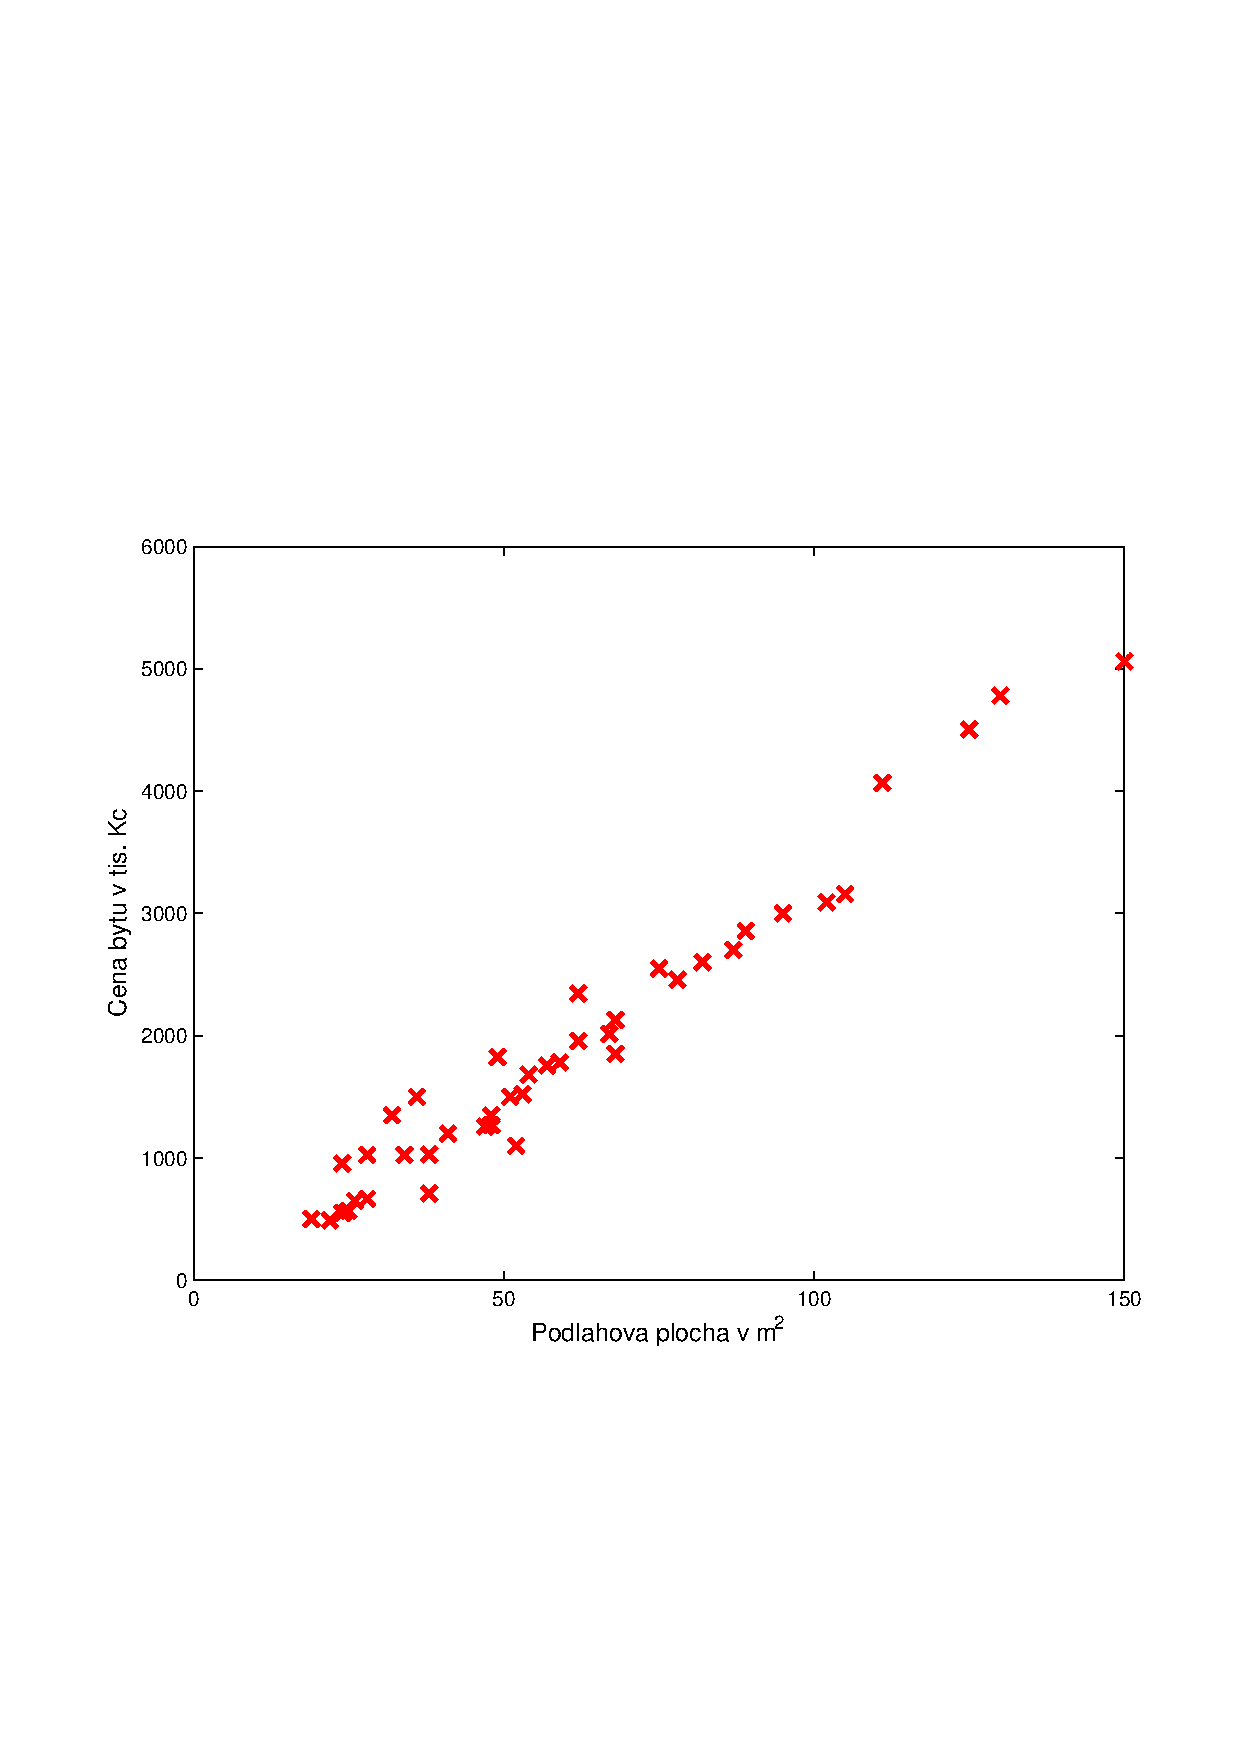
\includegraphics[scale = 0.5, trim = 3cm 7cm 3cm 9cm]{./Img/LinearniRegrese/cena_plocha.pdf}
	\caption{Vývoj ceny bytu v závislosti na podlahové ploše.}
	\label{fig:cena_plocha}
\end{figure}





%----------------UCENI-S-UCITELEM--------------------
\subsection{Učení s učitelem}
\label{sec:LinearniRegreseUceniSUcitelem}

\par{Učení s~učitelem (supervised learning) dává \uv{správnou odpověď} pro každý příklad z~množiny dat.}

\par{Problém regrese: Na základě reálného (spojitého) vstupu predikovat reálný (spojitý) výstup.}

\par{Problém klasifikace: Na základě diskrétního vstupu predikovat diskrétní výstup.}

\par{Více formálně v~případě učení s~učitelem potřebujeme množinu dat nazývanou trénovací množina. V~našem případě predikce ceny bytu máme trénovací množinu cen bytů a~k~nim odpovídající podlahovou plochu. Naším úkolem je naučit se z~těchto dat jak predikovat ceny bytů.}

\par{Nyní zavedeme notaci nechť $m$ je velikost trénovací sady, $x$ jsou \uv{vstupní} proměnné neboli příznaky a~$y$ jsou \uv{výstupní} proměnné neboli příznaky. Jeden trénovací vzorek budeme označovat jako $\left(\bm{x}, y \right)$ a~odpovídá jednomu řádku v~tabulce \ref{tab:vzorky}. Dále $\left( x^{\left( i \right)}, y^{\left( i \right)} \right)$ označuje $i$-tý trénovací vzorek.}

\begin{table}[!ht]
\centering
\begin{tabular}{c|c}
	{Velikost bytu v $m^2$ ($x$)} & {Cena bytu v tis. Kč ($y$)}\\
	\hline
	{19} & {500}\\
	{22} & {490}\\
	{25} & {568}\\
	{$\ldots$} & {$\ldots$}
\end{tabular}
\caption{Příklady trénovacích vzorků.}
\label{tab:vzorky}
\end{table}

\par{Trénovací množina, v~našem případě ceny bytů, je potřebná pro natrénování učícího se algoritmu, jehož výstupem je funkce (hypotézy), která se většinou označuje $h$. Účelem funkce (hypotézy) $h$ je ze vstupu $x$ (velikost bytu) odhadnout výstup $y$ (cena bytu). Tedy $h$ je funkce, která mapuje $x$ na $y$. Schéma je naznačeno na Obr. \ref{fig:schema}.}

\begin{figure}[!ht]
	\centering
	%trim option's parameter order: left bottom right top
	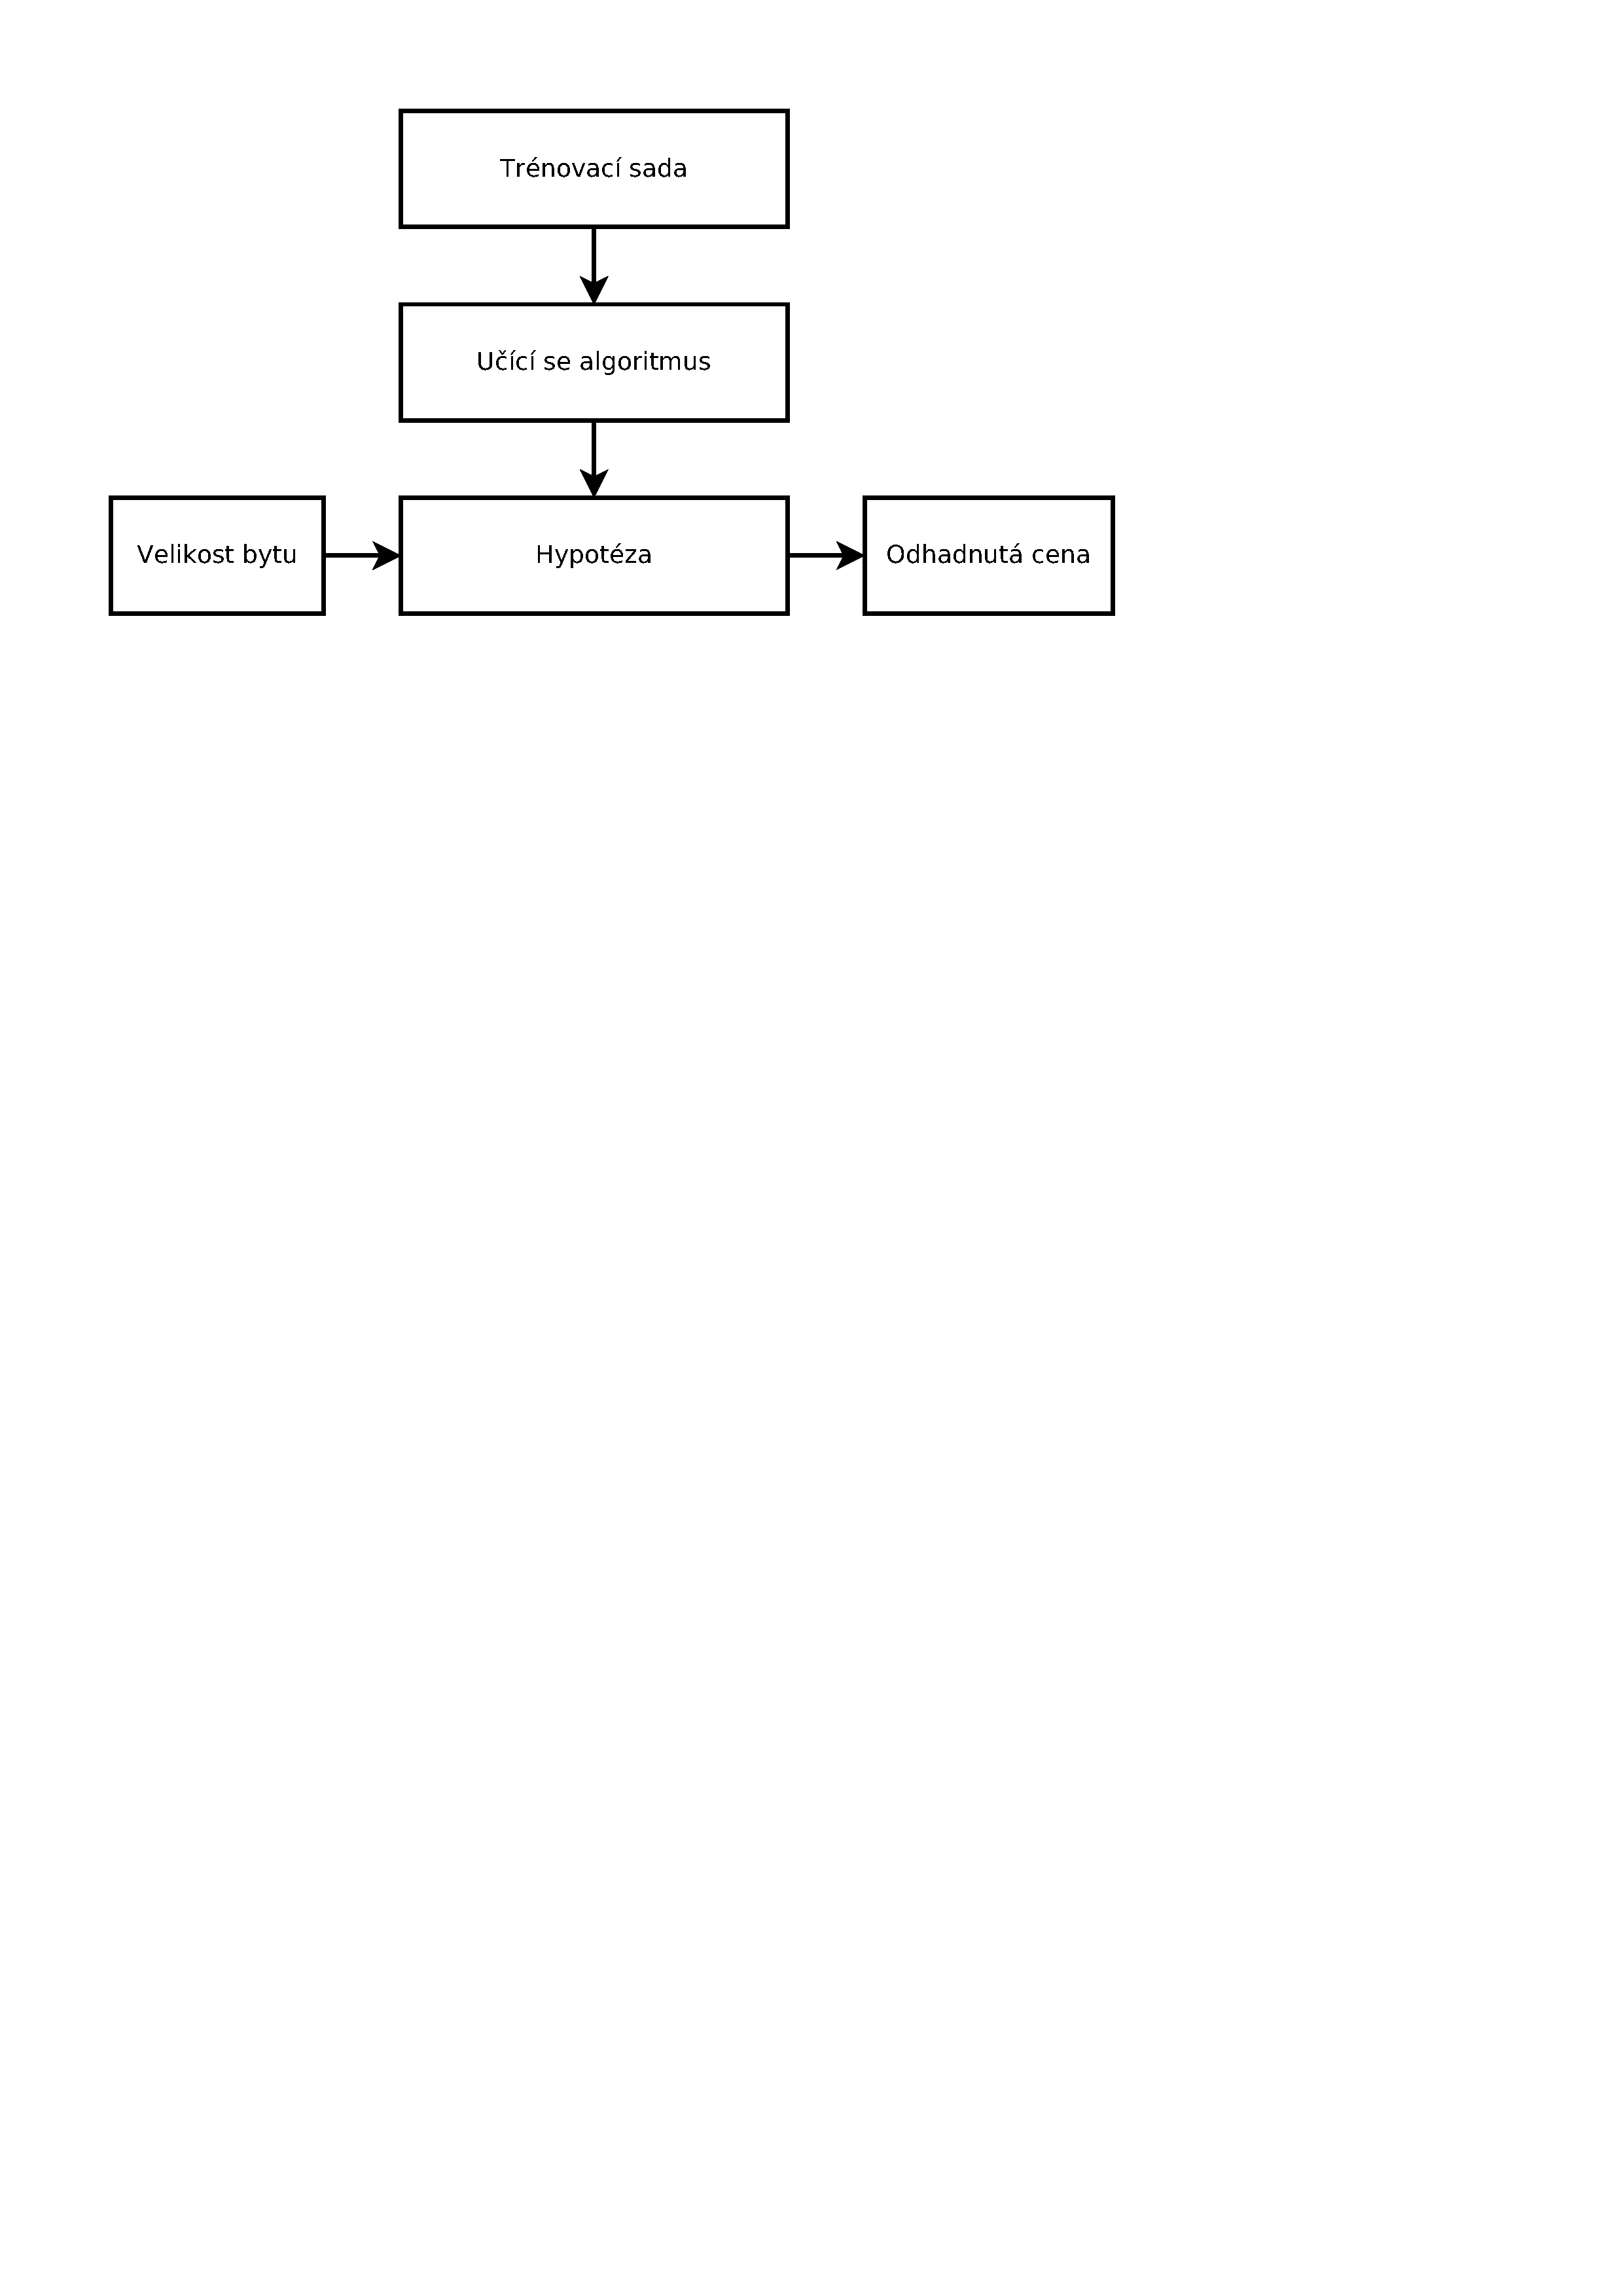
\includegraphics[scale = 0.5, trim = 3.5cm 42cm 14cm 2cm]{./Img/LinearniRegrese/schema.pdf}
	\caption{Schéma učení s učitelem.}
	\label{fig:schema}
\end{figure}

\par{Když navrhujeme učící se algoritmy, další věc kterou potřebujeme rozhodnout je jak budeme reprezentovat hypotézu $h$. V~našem motivačním příkladě si vystačíme s~hypotézou v~následujícím tvaru lineární funkce:
\begin{equation}
	h_{\bm{\Theta}} \left( x \right) = \vartheta_0 + \vartheta_1 x,
\end{equation}
zkráceně $h \left( x \right)$. Jedná se tedy o~lineární regresi s~jednou proměnnou. V~případě komplexnějšího učícího se algoritmu je nutné použít složitější nelineární model.}

\subsubsection*{Poznámka}
\par{$\vartheta$ je malá théta a $\Theta$ je velká théta.}

\newpage















%----------------ZTRATOVA-FUNKCE---------------------
\subsection{Ztrátová funkce}
\label{sec:LinearniRegreseZtratovaFunkce}

\par{Pro nejlepší napasování našeho lineárního modelu na trénovací data budeme potřebovat určit parametr $\vartheta_0$ a~$\vartheta_1$ v~naší hypotéze:
\begin{equation}
	h_{\bm{\Theta}} \left( x \right) = \vartheta_0 + \vartheta_1 x,
\end{equation}}

\par{Snažíme se zvolit parametry $\vartheta_0$ a $\vartheta_1$ tak, aby hypotéza $h_{\bm{\Theta}} \left( x \right)$ byla co nejblíže k $y$ pro naše trénovací vzorky $\left( x, y \right)$. Jinými slovy snažíme se minimalizovat kvadratickou chybu:

\begin{equation}
	\min_{\vartheta_0, \vartheta_1} \frac{1}{2m} \sum_{i = 1}^{m} \left( h_{\bm{\Theta}} \left( x^{\left( i \right)} \right) - y^{\left( i \right)} \right)^2,
\end{equation}
kde
\begin{equation}
	h_{\bm{\Theta}} \left( x^{\left( i \right)} \right) = \vartheta_0 + \vartheta_1 x^{\left( i \right)}.
	\label{eq:hProJednoDato}
\end{equation}
Přesněji označíme ztrátovou funkci:
\begin{equation}
	J \left( \vartheta_0, \vartheta_1 \right) = \frac{1}{2m} \sum_{i = 1}^{m} \left( h_{\bm{\Theta}} \left( x^{\left( i \right)} \right) - y^{\left( i \right)} \right)^2
\end{equation}
a minimalizujeme
\begin{equation}
	\min_{\vartheta_0, \vartheta_1} 	J \left( \vartheta_0, \vartheta_1 \right).
\end{equation}
Tato ztrátová funkce $J$ je také občas nazývána kvadratická chyba nebo ztrátová funkce kvadratické chyby.}

\par{Ztrátová funkce ve formě kvadratické chyby je nejčastěji používanou ztrátovou funkcí při řešení regresních problémů.}





\newpage








%----------------GRADIENT-DESCENT---------------------
\subsection{Gradientní algoritmus}
\label{sec:LinearniRegreseGradientDescent}

\par{V~kapitole \ref{sec:LinearniRegreseZtratovaFunkce} jsme definovali ztrátovou funkci $J$. V~této kapitole bude popsán gradientní algoritmus pro minimalizaci ztrátové funkce $J$. Gradientní algoritmus není omezen jen a~pouze na lineární regresi nalézá uplatnění v~optimalizaci a~v~dalších oblastech strojového učení.} 

\par{Máme ztrátovou funkci $J \left( \vartheta_0, \vartheta_1 \right)$ a~chtěli bychom jí minimalizovat. Proto zvolíme náhodně $\vartheta_0$ a~$\vartheta_1$, dále v~každé iteraci měníme hodnoty $\vartheta_0$ a~$\vartheta_1$, tak abychom redukovali $J \left( \vartheta_0, \vartheta_1 \right)$ dokud, v~nejlepším případě, nedokonvergujeme do globálního minima.}

\par{Obecně lze gradientní algoritmus použít na jakoukoliv ztrátovou funkci:
\begin{equation}
	J \left( \vartheta_0, \cdots, \vartheta_n \right)
\end{equation}
a snažíme se minimalizovat:
\begin{equation}
	\min_{\vartheta_0, \ldots, \vartheta_n} J \left( \vartheta_0, \ldots, \vartheta_n \right)
\end{equation}}

\par{Definice gradientního algoritmu: opakuj dokud není dosaženo konvergence
\begin{equation}
	\vartheta_j = \vartheta_j - \alpha \frac{\partial}{\partial \vartheta_j} J \left( \vartheta_0 , \vartheta_1 \right),
	\label{eq:gradDescentIter}
\end{equation}
pro $j = \{ 0, 1 \}$, pro náš příklad (lineární regrese jedné proměnné) v~sekci \ref{sec:LinearniRegreseMotivace}. V~rovnici \ref{eq:gradDescentIter} proměnná $\alpha$ určuje, jak velké kroky bude gradientní algoritmus dělat při hledání minima a~nazývá se rychlost učení. V~případě velké hodnoty $\alpha$ bude algoritmus postupovat velkými kroky, rychle, ale není zajištěna konvergence, jelikož se může stát, že algoritmus bude kroužit kolem minima, ale nedosáhne ho, nebo bude divergovat. V~případě malé hodnoty $\alpha$ bude algoritmus velice pomalý a~nemusí dosáhnout minima pro stanovený počet iterací. Gradientní algoritmus může konvergovat do lokálního minima v~případě, že je rychlost učení $\alpha$ konstantní. Proto se v~reálných aplikacích volí nejdříve větší $\alpha$, které se s~rostoucí hodnotou iterací nebo času zmenšuje.}

\subsubsection*{Poznámka}
\par{Pro implementaci: je nutné aktualizovat všechny $\Theta$ současně
\begin{eqnarray}
	&temp_0 &= \vartheta_0 - \alpha \frac{\partial}{\partial \vartheta_0} J \left( \vartheta_0 , \vartheta_1 \right),\\
	&temp_1 &= \vartheta_1 - \alpha \frac{\partial}{\partial \vartheta_1} J \left( \vartheta_0 , \vartheta_1 \right), \\
		&\vartheta_0 &= temp_0, \\
		&\vartheta_1 &= temp_1.
\end{eqnarray}}

\par{Nyní budeme aplikovat gradientní algoritmus na náš problém lineární regrese
\begin{equation}
	\frac{\partial}{\partial \vartheta_j} J \left( \vartheta_0, \vartheta_1 \right) = \frac{\partial}{\partial \vartheta_j} \cdot \frac{1}{2m} \sum_{i = 1}^{m} \left( h_{\bm{\Theta}} \left( x^{\left( i \right)} \right) - y^{\left( i \right)} \right)^2,
\end{equation}
po dosazení z~rovnice \ref{eq:hProJednoDato} dostáváme
\begin{equation}
	\frac{\partial}{\partial \vartheta_j} J \left( \vartheta_0, \vartheta_1 \right) = \frac{\partial}{\partial \vartheta_j} \cdot \frac{1}{2m} \sum_{i = 1}^{m} \left( \vartheta_0 + \vartheta_1  x^{\left( i \right)} - y^{\left( i \right)} \right)^2,
\end{equation}
po zderivování podle jednotlivých parametrů $\Theta$ získáme
\begin{eqnarray}
	\frac{\partial}{\partial \vartheta_0} &J \left( \vartheta_0, \vartheta_1 \right) &= \frac{1}{m} \sum_{i = 1}^{m} \left( h_{\bm{\Theta}} \left( x^{\left( i \right)} \right) - y^{\left( i \right)} \right),\\
	\frac{\partial}{\partial \vartheta_1} &J \left( \vartheta_0, \vartheta_1 \right) &= \frac{1}{m} \sum_{i = 1}^{m} \left( h_{\bm{\Theta}} \left( x^{\left( i \right)} \right) - y^{\left( i \right)} \right) x^{\left( i \right)}.
\end{eqnarray}}

\par{Výsledný konkrétní tvar rovnice \ref{eq:gradDescentIter} pro $\vartheta_0$ a $\vartheta_1$
\begin{eqnarray}
		&\vartheta_0 &= \vartheta_0 - \alpha \frac{1}{m} \sum_{i = 1}^{m} \left( h_{\bm{\Theta}} \left( x^{\left( i \right)} \right) - y^{\left( i \right)} \right),\\
		&\vartheta_1 &= \vartheta_1 - \alpha \frac{1}{m} \sum_{i = 1}^{m} \left( h_{\bm{\Theta}} \left( x^{\left( i \right)} \right) - y^{\left( i \right)} \right) x^{\left( i \right)}.
\end{eqnarray}}

\par{Gradientnímu algoritmu popsanému výše se také někdy říká dávkový gradientní algoritmus, protože využívá všechna trénovací data, při součtu přes všech $m$ vzorků, v~každém kroku.}

\begin{figure}[!ht]
	\centering
	%trim option's parameter order: left bottom right top
	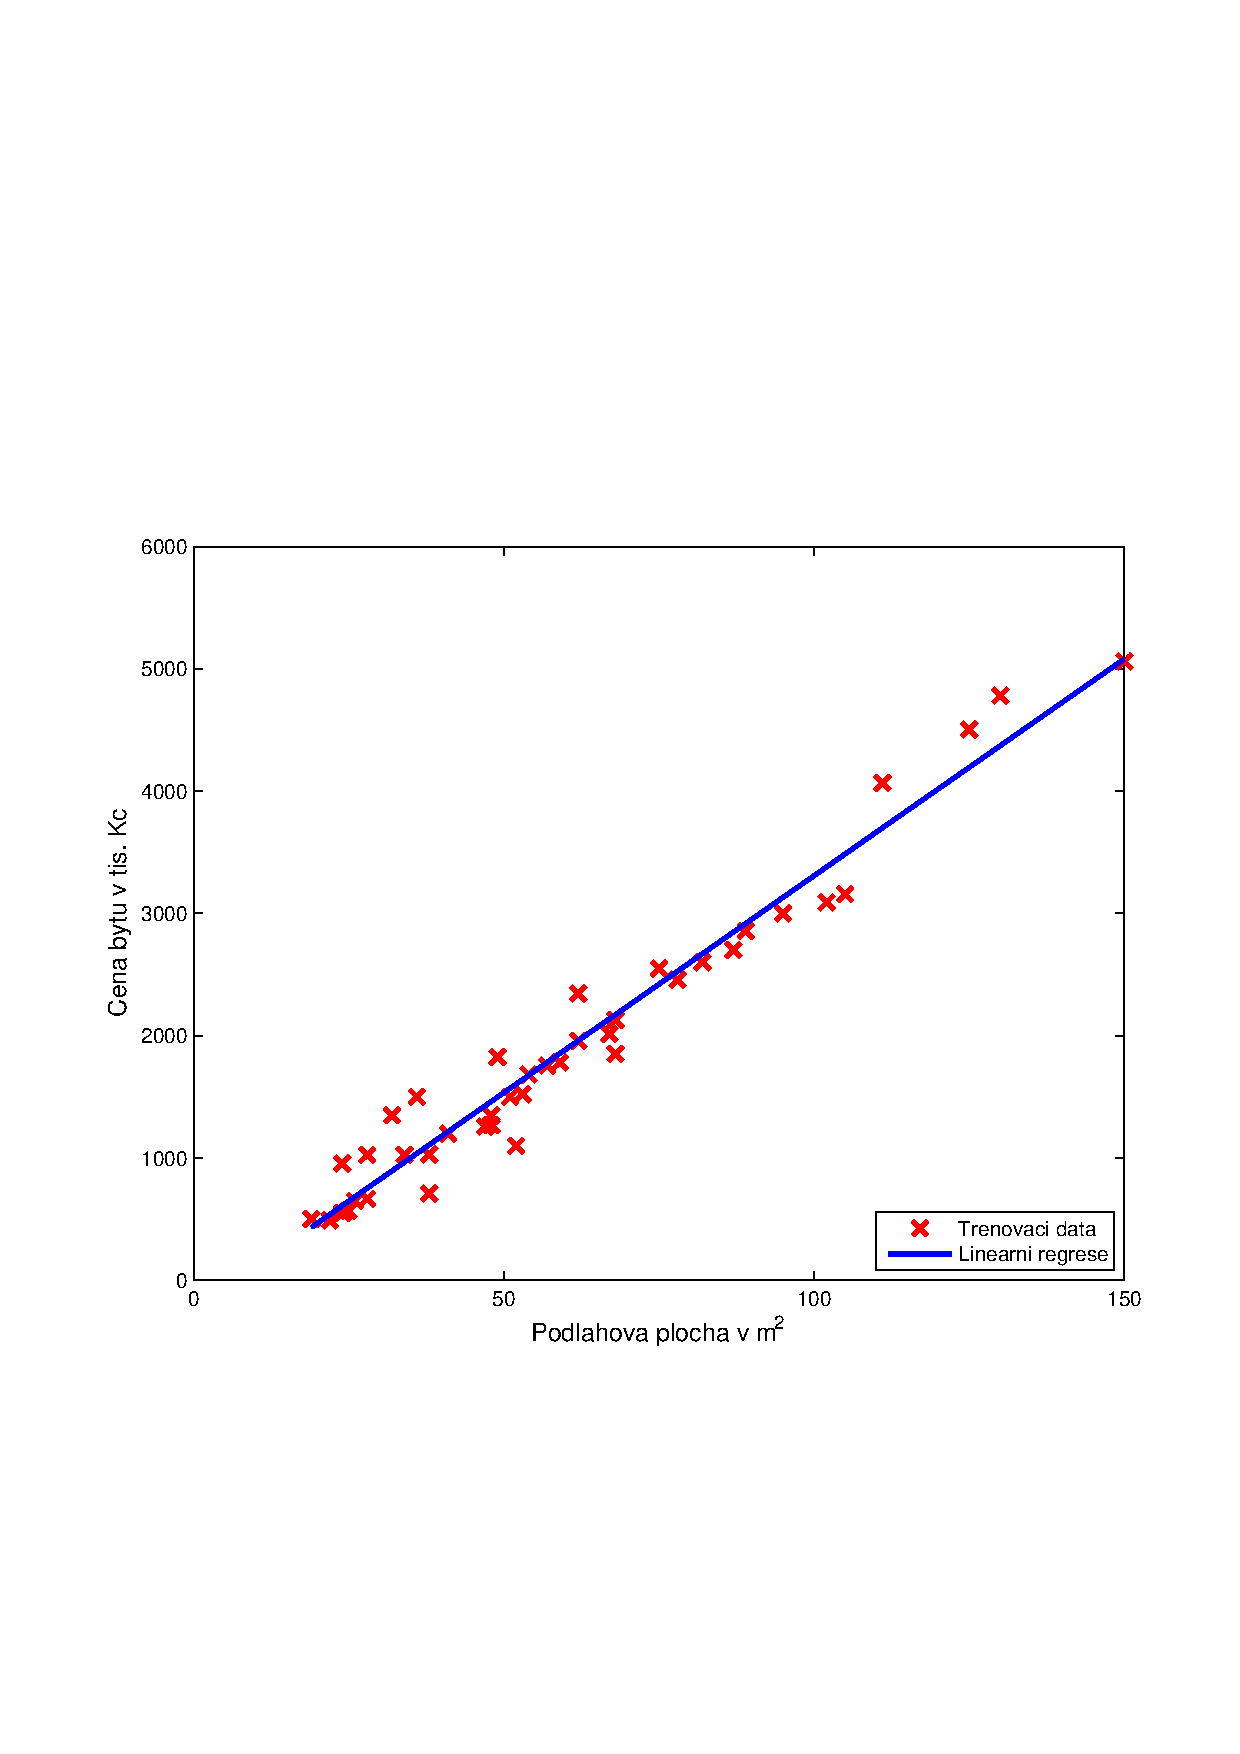
\includegraphics[scale = 0.5, trim = 2.5cm 7cm 2cm 9cm]{./Img/LinearniRegrese/cena_plocha_linear_regrese.pdf}
	\caption{Výsledná lineární regrese našeho úvodního příkladu po výpočtu gradientním algoritmem.}
	\label{fig:cena_plocha_linear_regrese}
\end{figure}


\newpage









%----------------VICEROZMERNA-LINEARNI-REGRESE-------------------
\subsection{Vícerozměrná lineární regrese}
\label{sec:LinearniRegreseVicePromennych}

\par{V sekci \ref{sec:LinearniRegreseUceniSUcitelem} byla představena lineární regrese o~jedné proměnné na příkladě predikce ceny bytu (výstup $y$) v závislosti na velikosti podlahové plochy $m^2$ (vstup $x$).}

\par{V případě vícerozměrné lineární regrese si můžeme představit, že nemáme pouze velikost podlahové plochy bytu, ale výsledná cena závisí i dalších parametrech bytu, viz tabulka \ref{tab:vzorkyND}.

\begin{table}[!ht]
\centering
\begin{tabular}{c|c|c|c|c}
	{Velikost bytu} & {Počet místností} & {Počet poschodí} & {Stáří bytu} & {Cena bytu}\\
	{$x_1$} & {$x_2$} & {$x_3$} & {$x_4$} & {$y$}\\
	\hline
	{19} & {5} & {1} & {45} & {500}\\
	{22} & {3} & {2} & {40} & {490}\\
	{25} & {2} & {1} & {30} & {568}\\
	{$\ldots$} & {$\ldots$} & {$\ldots$} & {$\ldots$} & {$\ldots$}
\end{tabular}
\caption{Příklady vícerozměrných trénovacích vzorků.}
\label{tab:vzorkyND}
\end{table}}

\par{Proměnnou $n$ budeme označovat počet příznaků (v~našem případě v tabulce \ref{tab:vzorkyND} $x_{1, \ldots , 4}$, proto $n = 4$.) Dále budeme stále jako u jednorozměrného případu označovat vstupní příznaky (všechny = sloupcový vektor) $\bm{x}^{\left( i \right)}$ pro $i$-tý trénovací vzor. A~hodnota jednotlivého $j$-tého příznaku $i$-tého trénovacího vzoru bude označována $\bm{x}^{\left( i \right)}_{j}$.}

\par{V~případě jednorozměrné lineární regrese byla naše hypotéza $h_\Theta$ reprezentována
\begin{equation}
	h_{\bm{\Theta}} \left( x \right) = \vartheta_0 + \vartheta_1 x,
	\label{eq:1Dhypothesis}
\end{equation}
v~našem vícerozměrném případě nabývá tvaru
\begin{equation}
	h_{\bm{\Theta}} \left( \bm{x} \right) = \vartheta_0 + \vartheta_1 x_1 + \vartheta_2 x_2 + \vartheta_3 x_3 + \vartheta_4 x_4 .
	\label{eq:NDhypothesis}
\end{equation}
V~případě \ref{eq:1Dhypothesis} i \ref{eq:NDhypothesis} je možné si všimnout, že $x_0 = 1$ čehož dále využijeme, přesněji $\bm{x}^{\left( i \right)}_0 = 1$ z důvodu dodržení konvence. Proto $\bm{x} \in \mathrm{R}^{n + 1}$ a to samé platí pro parametry $\bm{\Theta} \in \mathrm{R}^{n + 1}$.}

\subsubsection*{Poznámka}
\par{V~našem příkladě odpovídají
\begin{equation}
	\bm{x} = \left[ x_0,~x_1,~x_2,~x_3,~x_4 \right]^{\top}
\end{equation}
a
\begin{equation}
	\bm{\Theta} = \left[ \vartheta_0,~\vartheta_1,~\vartheta_2,~\vartheta_3,~\vartheta_4 \right]^{\top}.
\end{equation}}

\par{Obecněji lze vícerozměrnou hypotézu zapsat jako
\begin{equation}
	h_{\bm{\Theta}} \left( \bm{x} \right) = \vartheta_0 + \vartheta_1 x_1 + \vartheta_2 x_2 + \ldots + \vartheta_n x_n,
	\label{eq:NDhypothesisObecne}
\end{equation}
neboli jednoduše jako součin vektorů (vnitřní produkt)
\begin{equation}
	h_{\bm{\Theta}} \left( \bm{x} \right) = \bm{\Theta}^{\top} \bm{x}.
	\label{eq:NDhypothesisObecneVektorove}
\end{equation}}


\newpage












%----------------GRADIENT-DESCENT-VICEROZMERNY--------------------
\subsection{Gradientní algoritmus - vícerozměrná verze}
\label{sec:LinearniRegreseGradientDescentVicerozmerny}

\par{Budeme potřebovat hypotézu
\begin{equation}
	h_{\bm{\Theta}} \left( \bm{x} \right) = \bm{\Theta}^{\top} \bm{x} = \vartheta_0 x_0 + \vartheta_1 x_1 + \vartheta_2 x_2 + \ldots + \vartheta_n x_n,
\end{equation}
kde $x_0 = 1$, dále parametry $\bm{\Theta} = \left[ \vartheta_0,~\vartheta_1,~\vartheta_2,~\ldots,~\vartheta_4 \right]^{\top}$ a vícerozměrnou ztrátovou funkci
\begin{equation}
	J \left( \bm{\Theta} \right) = \frac{1}{2m} \sum_{i = 1}^{m} \left( h_{\bm{\Theta}} \left( \bm{x}^{\left( i \right)} \right) - y^{\left( i \right)} \right)^2.
\end{equation}}

\par{Gradientní algoritmus pak bude mít tvar: opakuj
\begin{equation}
	\vartheta_j = \vartheta_j - \alpha \frac{\partial}{\partial \vartheta_j} J \left( \bm{\Theta} \right),
	\label{eq:algoritmusNDgradientDescent}
\end{equation}
současně aktualizovat parametry pro všechny $j = 0, \ldots, n$.}

\par{Vztah z rovnice \ref{eq:algoritmusNDgradientDescent} lze zapsat jako
\begin{equation}
	\frac{\partial}{\partial \vartheta_j} J \left( \bm{\Theta} \right) = \frac{1}{m} \sum_{i = 1}^{m} \left( h_{\bm{\Theta}} \left( \bm{x}^{\left( i \right)} \right) - y^{\left( i \right)} \right) \bm{x}^{\left( i \right)}_j
	\label{eq:derivaceNDgradientDescent}	
\end{equation}
a po spojení rovnic 	\ref{eq:algoritmusNDgradientDescent} a \ref{eq:derivaceNDgradientDescent} získáváme výsledný tvar
\begin{equation}
	\vartheta_j = \vartheta_j - \alpha \frac{1}{m} \sum_{i = 1}^{m} \left( h_{\bm{\Theta}} \left( \bm{x}^{\left( i \right)} \right) - y^{\left( i \right)} \right) \bm{x}^{\left( i \right)}_j,
	\label{eq:NDgradientDescentVysledna}
\end{equation}
pokud bychom výslednou rovnici \ref{eq:NDgradientDescentVysledna} rozepsali pro první dva parametry $\vartheta_0$ a $\vartheta_1$ dostali bychom
\begin{eqnarray}
	&\vartheta_0 &= \vartheta_0 - \alpha \frac{1}{m} \sum_{i = 1}^{m} \left( h_{\bm{\Theta}} \left( \bm{x}^{\left( i \right)} \right) - y^{\left( i \right)} \right) \bm{x}^{\left( i \right)}_0, \quad \bm{x}^{\left( i \right)}_0 = 1\\
	&\vartheta_1 &= \vartheta_1 - \alpha \frac{1}{m} \sum_{i = 1}^{m} \left( h_{\bm{\Theta}} \left( \bm{x}^{\left( i \right)} \right) - y^{\left( i \right)} \right) \bm{x}^{\left( i \right)}_1\\
	\nonumber
	&\vdots
\end{eqnarray}}




\newpage









%----------------FEATURES-SCALING-------------------
\subsection{Features scaling}
\label{sec:featuresScaling}

\par{V~této podkapitole si řekneme něco o~velikosti příznaků. První a~nejdůležitější věcí je normování velikostí příznaků na stejnou velikost. Neboli, pokud použijeme opět náš příklad nákupu bytu a~definujeme si velikost bytu v~$dm^2$ (příznak $x_1$) a~počet místností bytu (příznak $x_2$) a~řekněme že:
\begin{eqnarray}
	\nonumber
	&x_1 &\in \langle 5000, 20000 \rangle,\\
	\nonumber
	&x_2 &\in \langle 1, 5 \rangle,
\end{eqnarray}
tak bude pro gradientní metodu velmi obtížné a~více výpočetně náročné (bude nutno spočítat více iterací) nalézt minimum. Proto je důležité, aby všechny příznaky měli stejné škálování. V~našem případě by to znamenalo 

\begin{eqnarray}
	\nonumber
	&x_1 &= \frac{\mbox{velikost bytu}}{20000},\\
	\nonumber
	&x_2 &= \frac{\mbox{počet místností}}{5}.
\end{eqnarray}
Více obecně lze říci, že se většinou volí normování na interval $\langle -1, 1 \rangle$.}

\subsubsection*{Mean normalization}
\par{Velice častá normalizace střední hodnotou $\mu$, konkrétně pro $i$-tý příznak
\begin{equation}
	x_i \leftarrow \frac{x_i - \mu_i}{max - min}
\end{equation}
nebo
\begin{equation}
	x_i \leftarrow \frac{x_i - \mu_i}{std}
\end{equation}
($std$ = Standard deviation).

















%----------------NORMAL-EQUATION------------------
\subsection{Analytické řešení}
\label{sec:normalEquation}

\par{V této sekci si ukážeme jak lze vypočítat minimum naší ztrátové funkce $J \left( \bm{\Theta} \right)$ analyticky.}

\subsubsection*{Příklad:}
\par{Předpokládejme 1D příklad ($\vartheta \in \mathcal{R}$), kdy máme ztrátovou funkci $J \left( \vartheta \right)$, která je funkcí jedné reálné proměnné
\begin{equation}
	J \left( \vartheta \right) = a \vartheta^2 + b \vartheta + c
\end{equation}}

\par{Pro minimalizaci naší kvadratické ztrátové funkce využijeme hledání extrému (položíme derivaci rovnou nule)
\begin{equation}
	\frac{\mathrm{d}}{\mathrm{d}\vartheta} J \left( \vartheta \right) = \ldots \equiv 0
\end{equation}
a vyřešíme pro parametr $\vartheta$.}

\par{Více obecněji pro $\bm{\Theta} \in \mathcal{R}^{n+1}$ bude naše ztrátová funkce nabývat tvaru
\begin{equation}
	J \left( \vartheta_0,~\vartheta_1,~\ldots,~\vartheta_m \right) = \frac{1}{2m} \sum_{i=1}^{m} \left( h_{\bm{\Theta}} \left( \bm{x}^{\left( i \right)} \right) - y^{\left( i \right)} \right)^2
\end{equation}
dále položíme parciální derivace podle jednotlivých parametrů rovny nule (pro všechny $j$)
\begin{equation}
	\frac{\partial}{\partial \vartheta_j} = \ldots \equiv 0
\end{equation}
a vyřešíme pro parametry $\vartheta_0,~\vartheta_1,~\ldots,~\vartheta_m$.}

\par{Pro složení obyčejné rovnice budeme potřebovat matici $\bm{X} \in \mathcal{R}^{m \times \left( n + 1 \right)}$, která v řádcích obsahuje jednotlivé vektory $\left( \bm{x}^{\left( i \right)} \right)^{\top}$ a výstupní sloupcový vektor $\bm{y} \in \mathcal{R}^{m}$. Kde $m$ je počet trénovacích vzorků (velikost trénovací množiny) a $n$ je počet příznaků, kde $\bm{x}_0^{\left( i \right)} = 0$.}

\par{Nyní můžeme zapsat předpis pro výpočet parametrů $\bm{\Theta}$ analyticky
\begin{equation}
	\bm{\Theta} = \left( \bm{X}^{\top} \bm{X} \right)^{-1} \bm{X}^{\top} \bm{y}.
\end{equation}
Pro analytické řešení není nutné příznaky normovat, jako v případě gradientního algoritmu, na stejné měřítko, jak je popsáno v sekci \ref{sec:featuresScaling}.}





















%----------------NORMAL-EQUATION------------------
\subsection{Gradientní algoritmus vs. analytické řešení}
\label{sec:GAvsAR}

\par{V této sekci budou zmíněny výhody a nevýhody gradientního algoritmu versus analytického řešení. Velikost trénovací množiny $m$ a počet příznaků $n$.
\begin{center}
\begin{tabular}{c|c}
	{Gradientní algoritmus} & {Analytické řešení} \\
	\hline
	{Nutno zvolit konstantu učení $\alpha$.} & {Není nutné volit konstantu učení $\alpha$.}\\
	{Potřebuje mnoho iterací.} & {Nepotřebuje iterovat.}\\
	{Pracuje dobře, když je $n$ velké.} & {Pomalé pokud je $n$ velké.}\\
	{~} & {Nutnost vypočítat inverzi $\left( \bm{X}^{\top} \bm{X} \right)^{-1}$.}\\
	{~} & {(Složitost $\mathcal{O}\left( n^3 \right)$).}\\
	{Zvolit pokud $n > 10^6$.} & {Zvolit pokud $n < 10^4$.}
\end{tabular}
\end{center}}


\newpage















%----BINARNI-REGRESE----------------------------------------------------------------


\section{Binární regrese - klasifikace}
\label{sec:BinarniRegrese}

\par{Logistická regrese je označení metody matematické statistiky zabývající se problematikou odhadu pravděpodobnosti nějakého jevu (závisle proměnné) na základě určitých známých skutečností (nezávisle proměnných), které mohou ovlivnit výskyt jevu. Událost, zda zkoumaný jev nastal, se modeluje pomocí náhodné veličiny, která nabývá hodnoty 0, pokud jev nenastal, nebo 1, pokud jev nastal.}











%------------KLASIFIKACE---------------------------------------------------------
\subsection{Klasifikace}
\label{sec:BinarniRegreseKlasifikace}

\par{Na úvod si uveďme několik klasifikačních příkladů:
\begin{center}
	\textbf{Spam:} je spam / není spam ?\\
	\textbf{Online transakce:} podvodné ano / ne ?\\
	\textbf{Nádor:} zhoubný / nezhoubný?
\end{center}
Z příkladů je zřejmé, že se jedná o rozhodnutí mezi dvěma možnostmi, tedy $y \in \{ 0, 1 \}$, kde $0$ je \uv{negativní třída} (nezhoubný nádor) a~$1$ je pozitivní třída (zhoubný nádor). Pokud máme $y \in \{ 0, 1 \}$ jedná se o~klasifikaci do dvou tříd, dále existuje klasifikace do více tříd, kde $y \in \{ 0, 1, 2, 3, \ldots \}$. V následujících kapitolách se budeme zabývat klasifikací do dvou tříd.}
\par{Nyní se dostáváme k problému jak vyvinout klasifikační algoritmus, což si můžeme ukázat na příkladu trénovací sady pro úlohu klasifikace nádorů. Nádor může být buď zhoubný nebo nezhoubný, tedy buďto 1 nebo 0. Dostupná data pro náš příklad jsou na obrázku \ref{fig:nadory1}.
\begin{figure}[!ht]
	\centering
	%trim option's parameter order: left bottom right top
	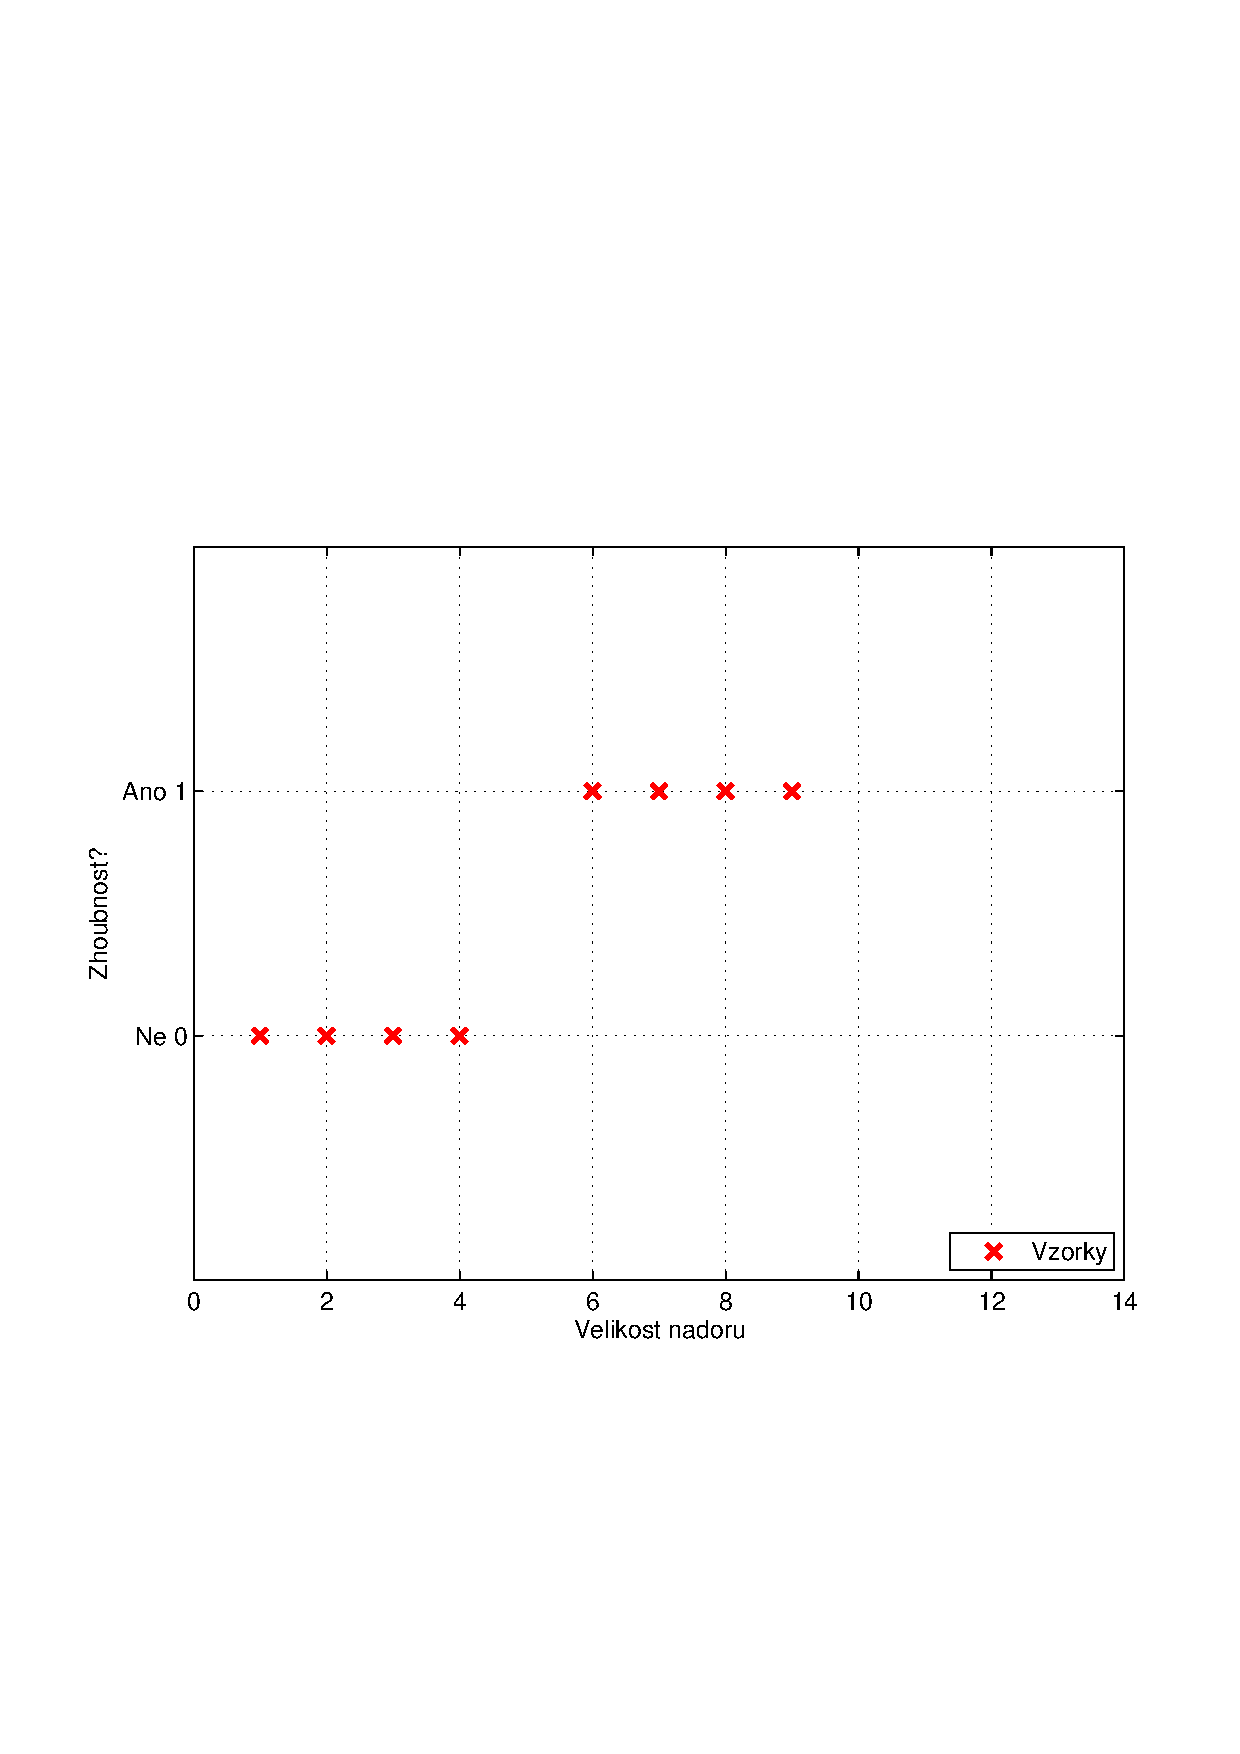
\includegraphics[width = 0.48\textwidth, trim = 2.5cm 7cm 2cm 9cm]{./Img/BinarniRegrese/prikladNadory/tumor_1st_example.pdf}
	\caption{Trénovací data.}
	\label{fig:nadory1}
\end{figure}}
\pagebreak

\par{Jedna z~věcí, kterou bychom mohli udělat, je aplikace algoritmu lineární regrese, který známe z~kapitoly \ref{sec:LinearniRegrese}. Výsledek aplikace hypotézy
\begin{equation}
	h_{\bm{\Theta}} \left( \bm{x} \right) = \bm{\Theta}^{\top} \bm{x}
\end{equation}
lze vidět na Obr. \ref{fig:nadory2}.}

\par{Pokud bychom chtěli udělat predikci ze získané hypotézy, tak můžeme využít klasifikátoru na základě prahování. Tedy hodnotu po jejíž překročení vzorek spadá již do druhé třídy, v~případě binární regrese je to hodnota 0.5. Chceme tedy určit
\begin{eqnarray}
	\label{eq:prah1}
	h_{\bm{\Theta}} \left( \bm{x} \right) \geq 0.5, \quad \mathrm{predikuj~} y = 1,\\
	\label{eq:prah2}
	h_{\bm{\Theta}} \left( \bm{x} \right) < 0.5, \quad \mathrm{predikuj~} y = 0.
\end{eqnarray}
Tento poznatek je reprezentován na Obr. \ref{fig:nadory3}.

\begin{figure}[!ht]
	\centering
	\begin{minipage}[t]{0.48\textwidth}
		%trim option's parameter order: left bottom right top
		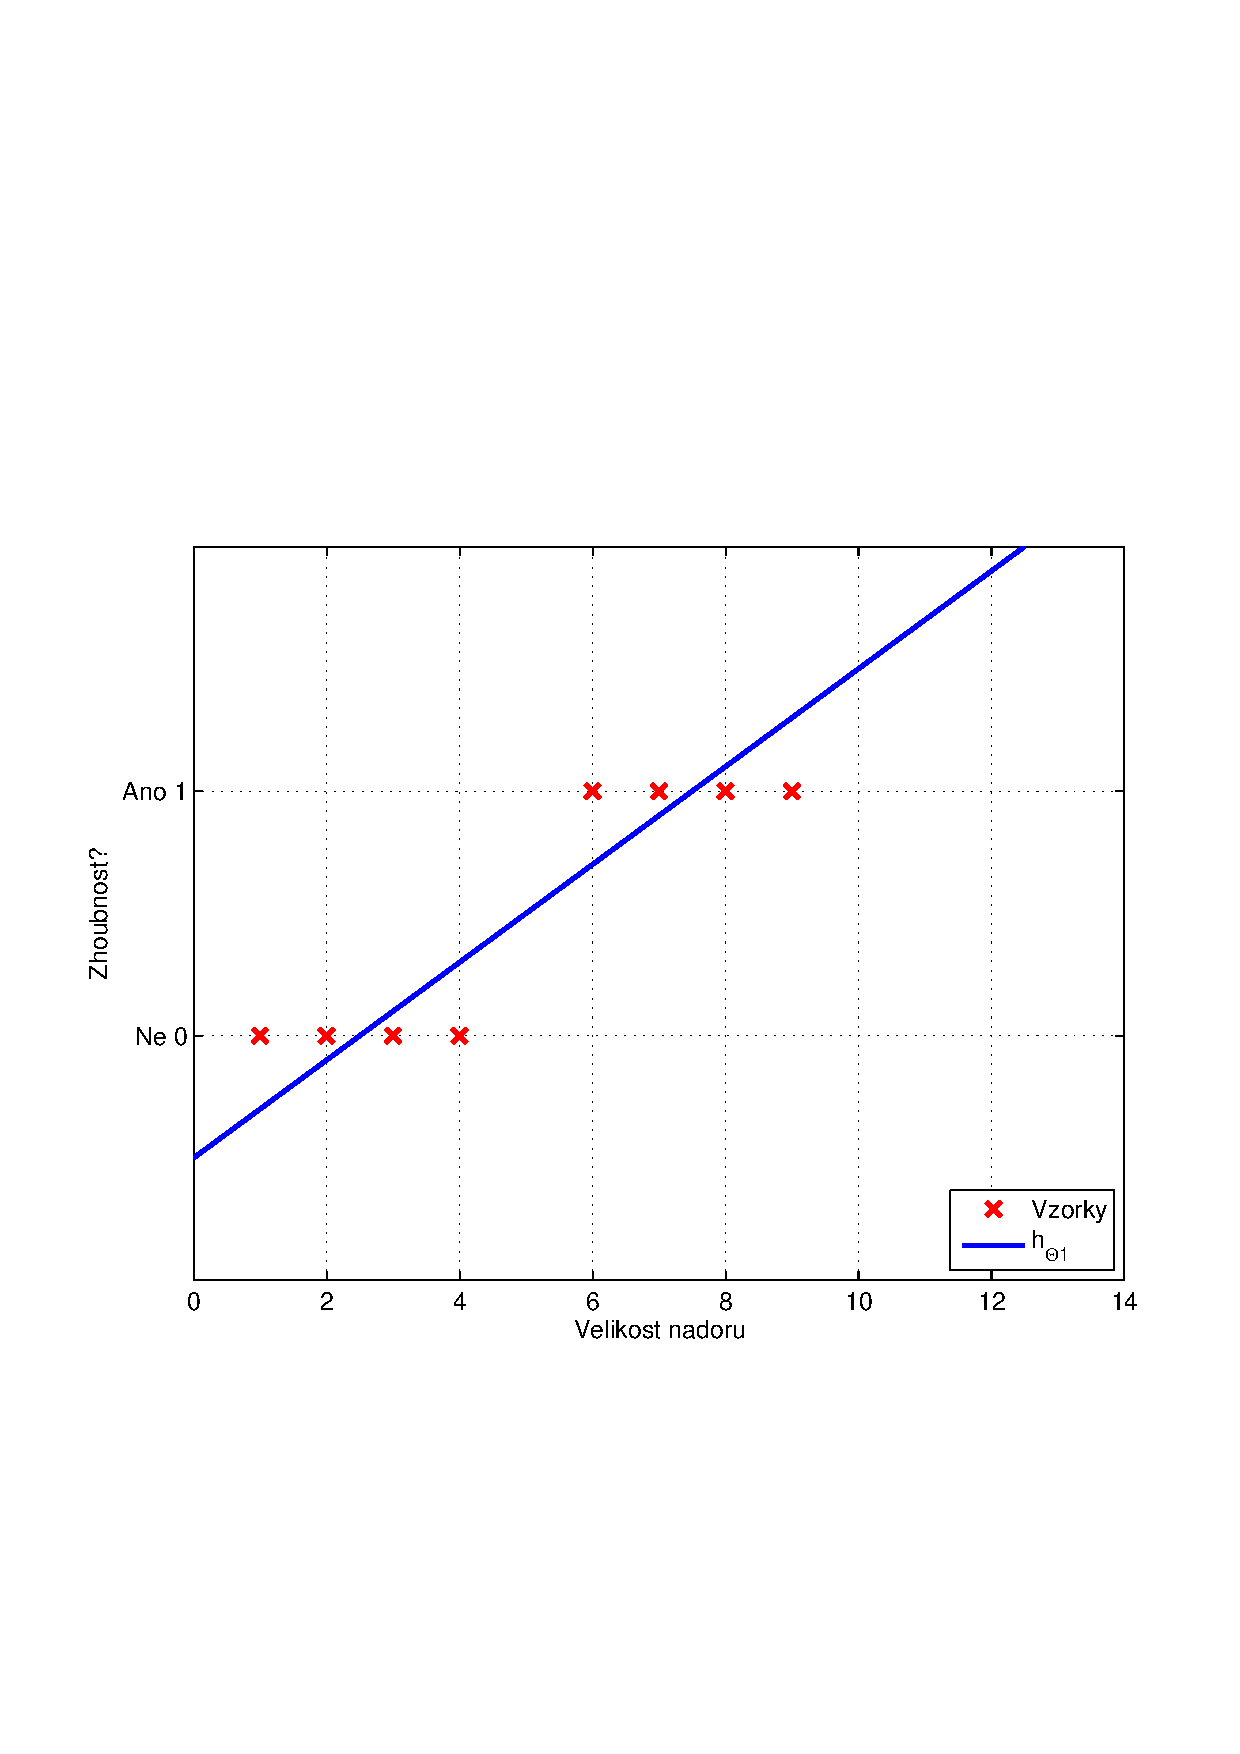
\includegraphics[width = \textwidth, trim = 2.5cm 7cm 2cm 9cm]{./Img/BinarniRegrese/prikladNadory/tumor_2st_example.pdf}
		\caption{Lineární regrese.}
		\label{fig:nadory2}
	\end{minipage}%
	\hfill
	\begin{minipage}[t]{0.48\textwidth}
		%trim option's parameter order: left bottom right top
		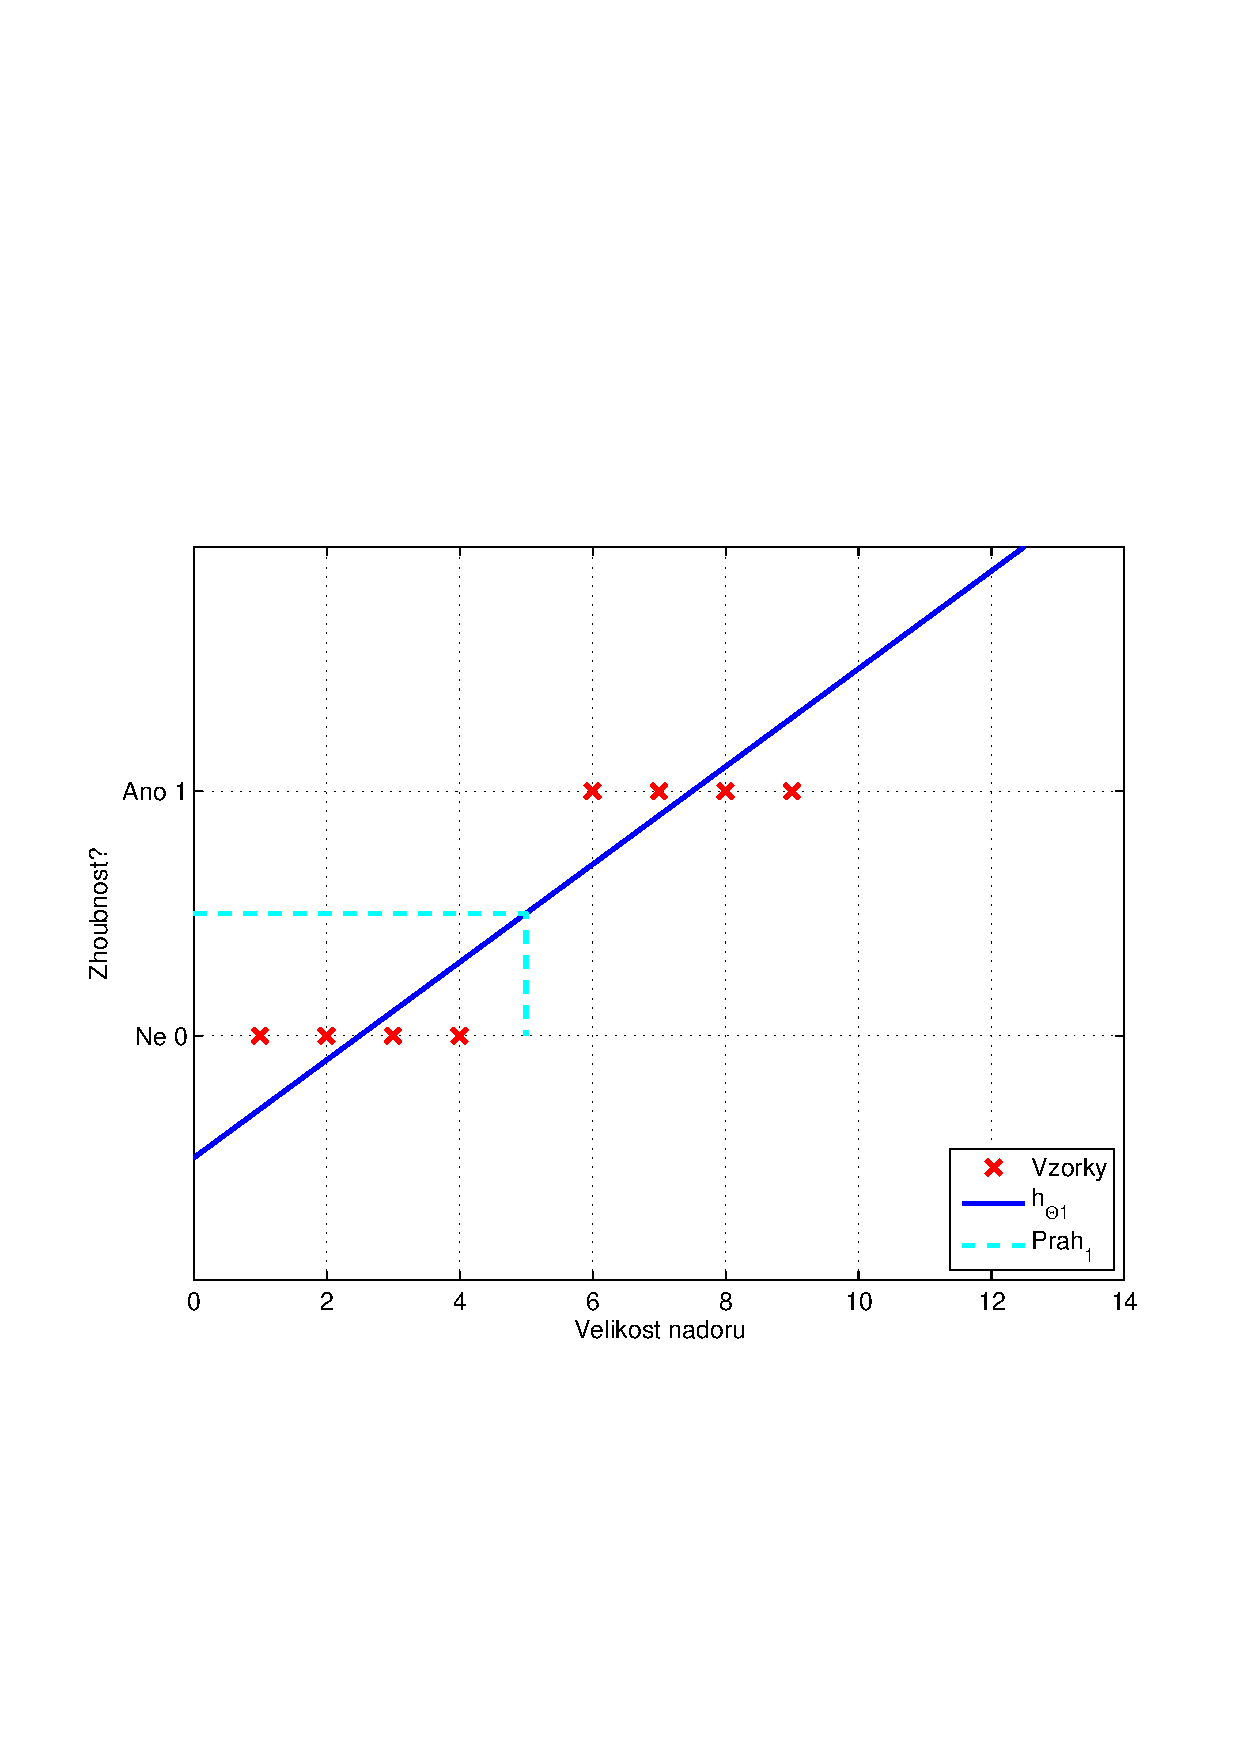
\includegraphics[width = \textwidth, trim = 2.5cm 7cm 2cm 9cm]{./Img/BinarniRegrese/prikladNadory/tumor_3st_example.pdf}
		\caption{Lineární regrese - určení rozhodovacího prahu.}
		\label{fig:nadory3}
	\end{minipage}%
\end{figure}}

\par{V tomto příkladě jsme si ukázali, že lineární regrese dělá něco co by se dalo považovat za řešení klasifikačního problému. Na následujícím rozšíření našeho příkladu bude ukázáno, že tomu tak není.}

\par{Rozšíříme náš příklad o~další vzorky viz Obr. \ref{fig:nadory4}, kde nám přibyly dva vzorky více vpravo. Po aplikování lineární regrese, na rozšířená data, získáváme výsledek, který lze vidět na Obr. \ref{fig:nadory5}. Aktuální hypotéza $h_{\bm{\Theta} 2}$ již nesplňuje podmínky definované vztahy \ref{eq:prah1} a~\ref{eq:prah2}, jelikož první vzorek, který má být vyhodnocen jako zhoubný by v tomto případě byl vyhodnocen jako nezhoubný, což může zásadně ovlivnit něčí život.

\begin{figure}[!ht]
	\centering
	\begin{minipage}[t]{0.48\textwidth}
		%trim option's parameter order: left bottom right top
		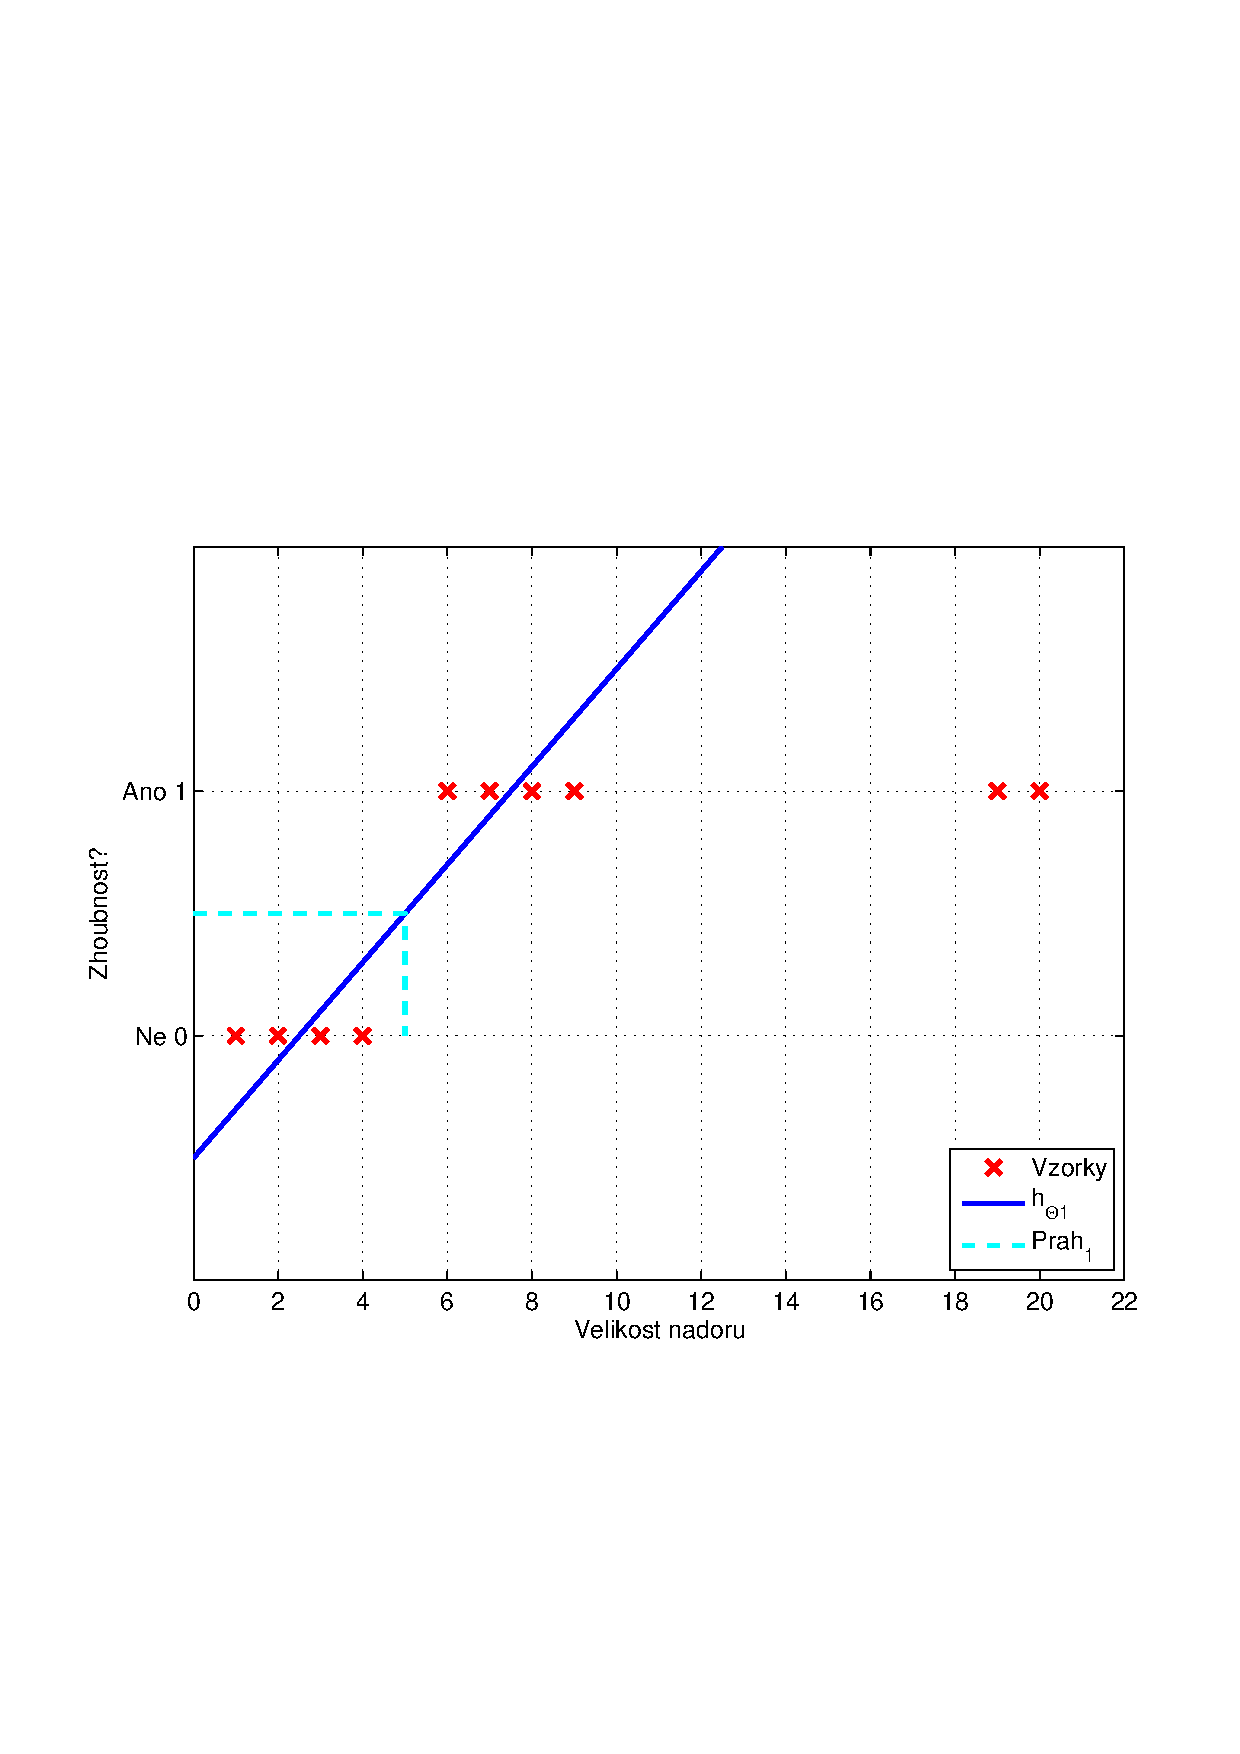
\includegraphics[width = \textwidth, trim = 2.5cm 7cm 2cm 9cm]{./Img/BinarniRegrese/prikladNadory/tumor_4st_example.pdf}
		\caption{Rozšíření trénovací množiny dat o dva vzorky vpravo.}
		\label{fig:nadory4}
	\end{minipage}%
	\hfill
	\begin{minipage}[t]{0.48\textwidth}
		%trim option's parameter order: left bottom right top
		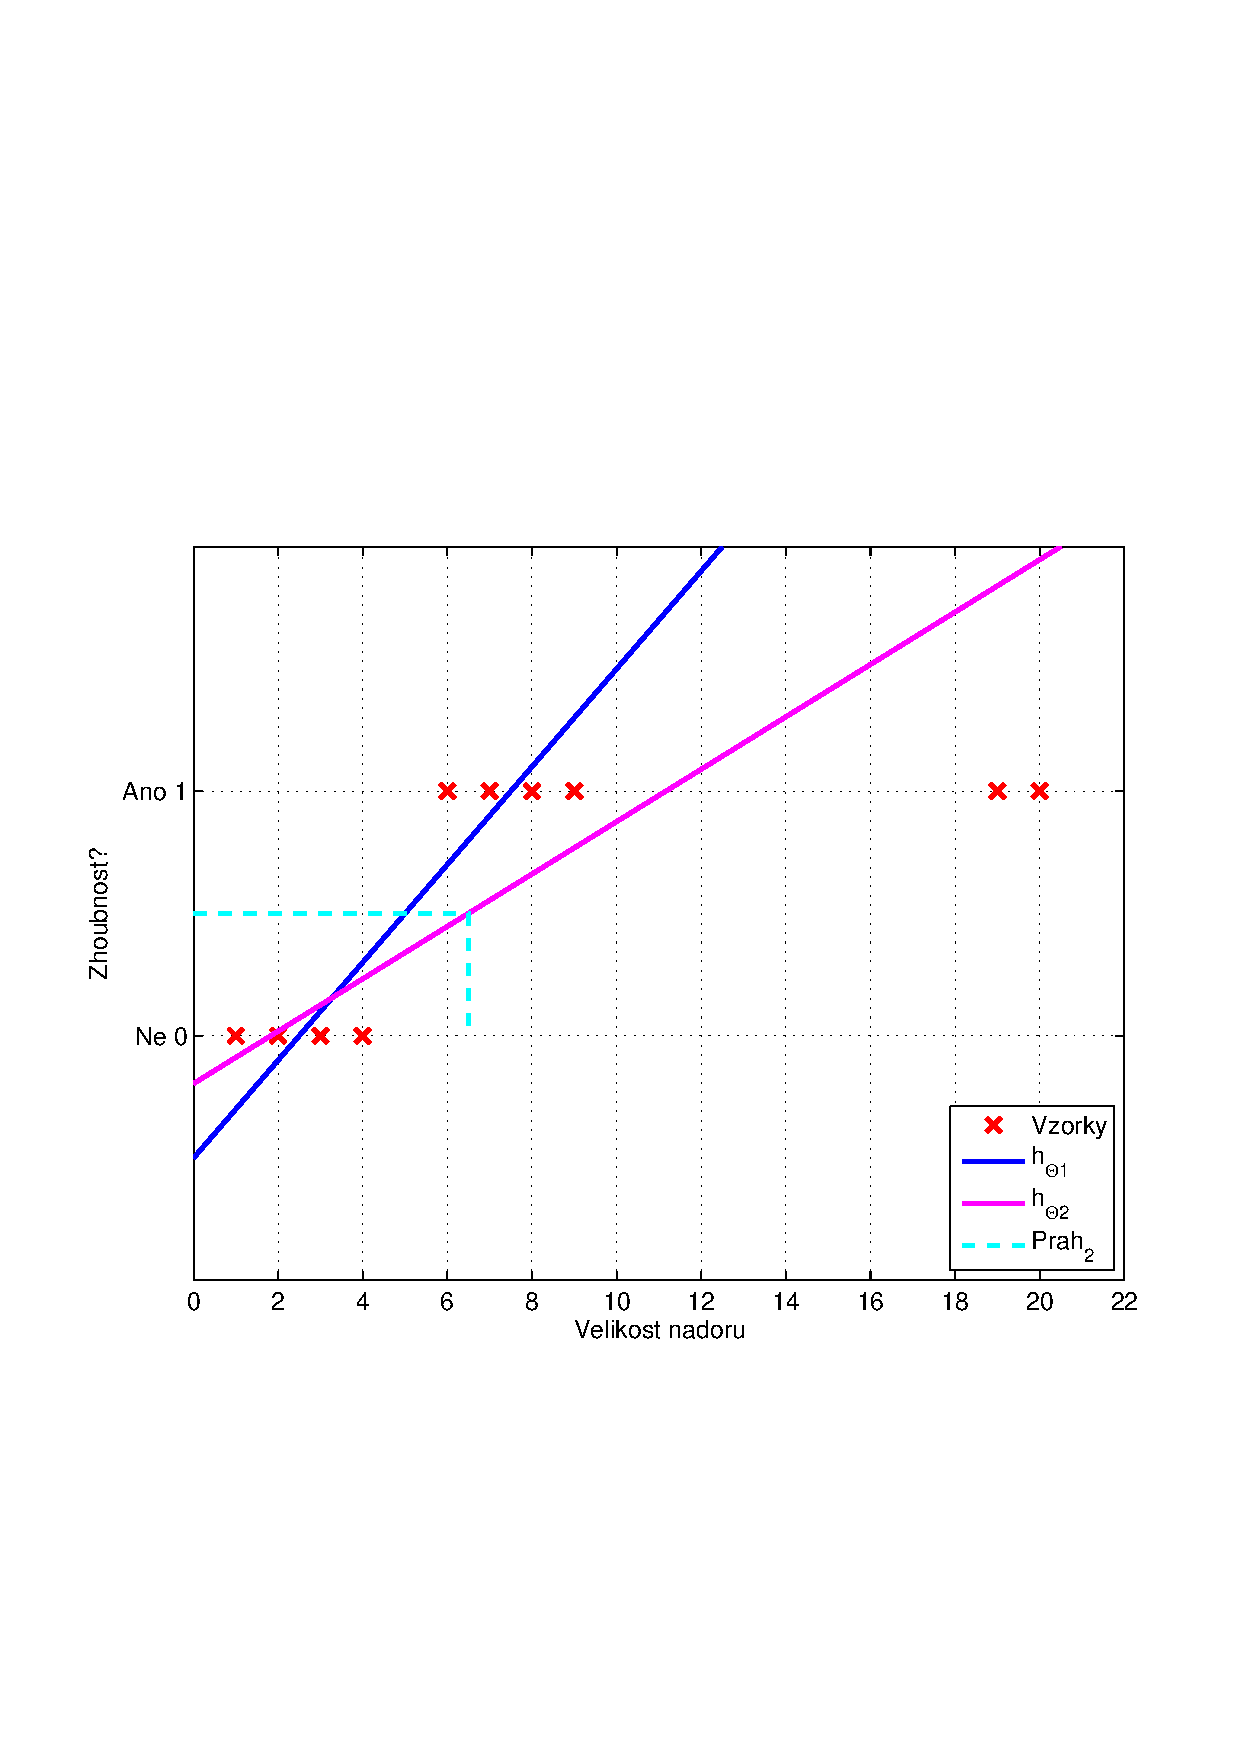
\includegraphics[width = \textwidth, trim = 2.5cm 7cm 2cm 9cm]{./Img/BinarniRegrese/prikladNadory/tumor_5st_example.pdf}
		\caption{Lineární regrese - určení rozhodovacího prahu a zobrazení jeho selhání při predikci.}
		\label{fig:nadory5}
	\end{minipage}%
\end{figure}}

\par{V tomto příkladě, lépe řečeno protipříkladě jsme si ukázali, proč je nevhodné využívat lineární regresi jako klasifikační algoritmus. Ve většině případů nefunguje správně. Pro klasifikaci na základě lineární regrese můžeme získat výsledek hypotézy $h_{\bm{\Theta}} > 1$ nebo $h_{\bm{\Theta}} < 0$, přičemž výsledek binární klasifikace je pouze $y = 0$ nebo $y = 0$. Proto bude nutné v~dalších kapitolách přijít se sofistikovanějším postupem binární regrese (klasifikace), která splňuje podmínku $0 \leq h_{\bm{\Theta}} \leq 1$.}




\newpage













%-----REPREZENTACE-HYPOTEZY-------------------------------------------------------------
\subsection{Reprezentace hypotézy}
\label{sec:BinarniRegreseReprezentaceHypotezy}

\par{V této kapitole si ukážeme, jak správně reprezentovat hypotézu, tedy jakou funkci je vhodné použít v případě problému klasifikace.}

\par{V sekci \ref{sec:BinarniRegreseKlasifikace} jsme zjistili, že bychom si pro binární regresní model přáli, aby platilo
\begin{equation}
	0 \leq h_{\bm{\Theta}} \left( \bm{x} \right) \leq 1,
\end{equation}
tedy aby výstupní hodnota byla mezi 0 a 1 (včetně). Pro reprezentaci hypotézy lineární regrese platí
\begin{equation}
	h_{\bm{\Theta}} \left( \bm{x} \right) = \bm{\Theta}^{\top} \bm{x},
\end{equation}
tuto hypotézu upravíme na tvar
\begin{equation}
	h_{\bm{\Theta}} \left( \bm{x} \right) = g \left( \bm{\Theta}^{\top} \bm{x} \right),
	\label{eq:Ghypoteza}
\end{equation}
kde funkce $g$ je definována následovně
\begin{equation}
	g \left( \bm{z} \right) = \frac{1}{1 + e^{-\bm{z}}},
	\label{eq:funkceSigmoidy}
\end{equation}
tato funkce se nazývá sigmoid funkce (Sigmoid function) nebo logistická/binární funkce (Logistic function). Jméno logistická funkce je důvod, proč vznik termín logistická/binární regrese. Pokud spojíme rovnice \ref{eq:Ghypoteza} a \ref{eq:funkceSigmoidy} získáme tvar
\begin{equation}
	h_{\bm{\Theta}} \left( \bm{x} \right) =  \frac{1}{1 + e^{- \bm{\Theta}^{\top} \bm{x}}} 
\end{equation}
a průběh grafu funkce $g \left( \bm{z} \right)$ lze vidět na Obr. \ref{fig:sigmoidFunction}.
\begin{figure}[!ht]
	\centering
	%trim option's parameter order: left bottom right top
	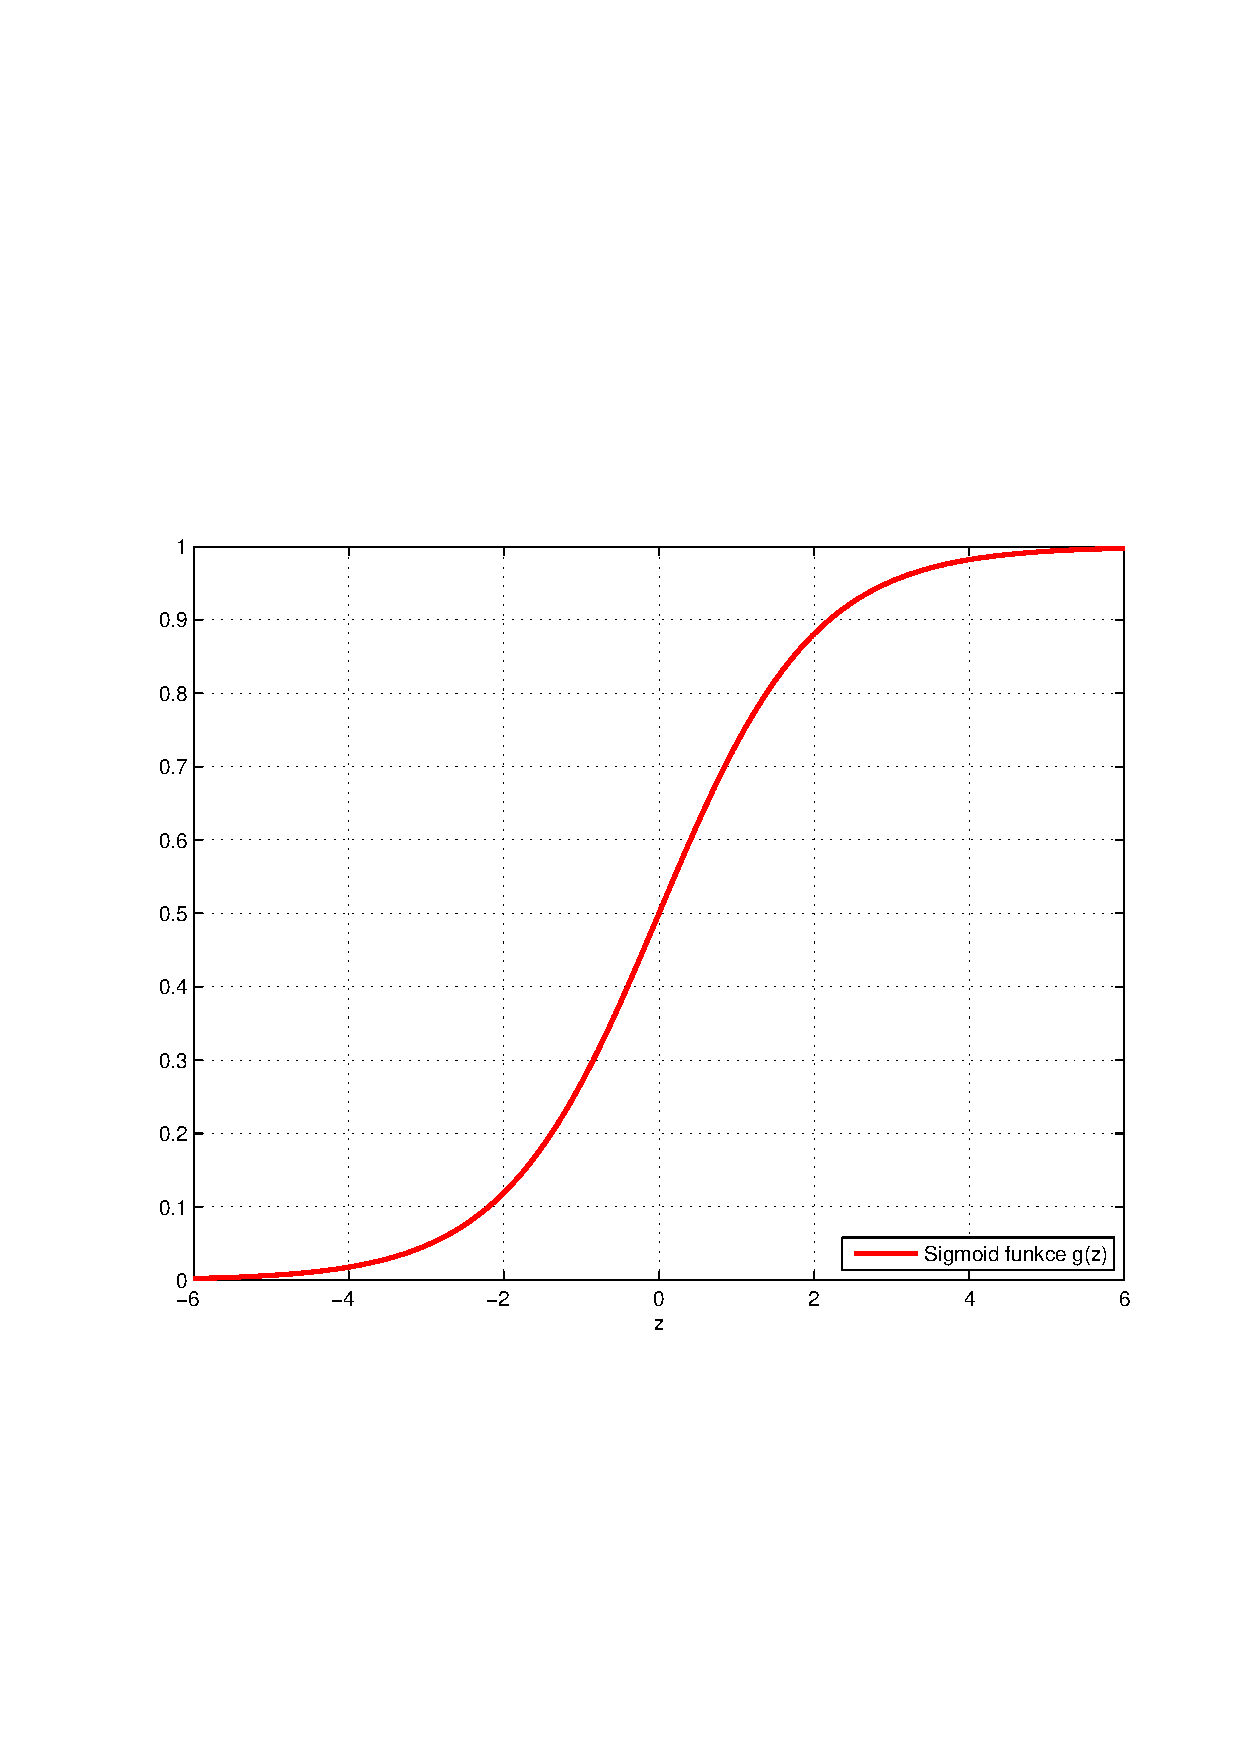
\includegraphics[width = 0.48\textwidth, trim = 2.5cm 7cm 2cm 9cm]{./Img/BinarniRegrese/sigmoidFunkce/sigmoidFunction.pdf}
	\caption{Sigmoidní funkce $g \left( z \right)$.}
	\label{fig:sigmoidFunction}
\end{figure}}
\par{Poznamenejme, že
\begin{eqnarray}
	\nonumber
	\lim_{z \to +\infty} &g \left( z \right) &= 1,\\
	\nonumber
	\lim_{z \to -\infty} &g \left( z \right) &= 0.
\end{eqnarray}}

\par{Nyní je potřeba, stejně jako dříve, přizpůsobit parametry $\bm{\Theta}$ našim datům, tedy pomocí trénovací množiny zvolit hodnoty parametrů $\bm{\Theta}$ a využít tyto parametry pro výpočet predikce.}

\par{Dále si povíme něco o interpretaci výstupu hypotézy. Hypotéza $h_{\bm{\Theta}} \left( \bm{x} \right) = $ odhadnutá pravděpodobnost, že výstup $y = 1$ na základě vstupních dat $\bm{x}$.}

\subsubsection*{Příklad}
\par{Pokud $\bm{x} = [ x_0,~x_1 ]^{\top} = [ 1,~$velikost nádoru$]^{\top}$ a $h_{\bm{\Theta}} \left( \bm{x} \right) = 0.7$, což říká pacientovi, že šance, že je nádor zhoubný je $70\%$. Nyní naše tvrzení zapíšeme formálněji
\begin{equation}
	h_{\bm{\Theta}} \left( \bm{x} \right) = P \left( y = 1 | \bm{x} ; \bm{\Theta} \right),
\end{equation}
neboli, pravděpodobnost, že $y = 1$, \uv{na základě dat $\bm{x}$}, parametrizovaná parametry $\bm{\Theta}$. V případě klasifikace víme, že výstup $y$ může nabývat pouze hodnot 0 nebo 1, proto platí
\begin{equation}
	P \left( y = 0 | \bm{x} ; \bm{\Theta} \right) + P \left( y = 1 | \bm{x} ; \bm{\Theta} \right) = 1,
\end{equation}
neboli
\begin{equation}
	P \left( y = 0 | \bm{x} ; \bm{\Theta} \right) = 1 - P \left( y = 1 | \bm{x} ; \bm{\Theta} \right).
\end{equation}}

\subsubsection*{Poznámka}
\par{Pravděpodobnost může nabývat hodnot $0-1$, neboli $0-100\%$.}





\newpage












%----------ROZHODOVACI-HRANICE-------------------------------------------------------------
\subsection{Rozhodovací hranice}
\label{sec:BinarniRegreseRozhodovaciHranice}

\par{V~této kapitole si povíme něco o~rozhodovací hranici, abychom získali větší ponětí o~výpočtu hypotézy binární regrese (klasifikace).}

\par{V kapitole \ref{sec:BinarniRegreseReprezentaceHypotezy} jsme si ukázali tvar hypotézy (sigmoid funkce)
\begin{equation}
	h_{\bm{\Theta}} \left( \bm{x} \right) = g \left( \bm{\Theta}^{\top} \bm{x} \right),
\end{equation}
kde
\begin{equation}
	g \left( \bm{z} \right) = \frac{1}{1 + e^{-\bm{z}}}
\end{equation}
a graf lze vidět na Obr. \ref{fig:sigmoidFunction2}.
\begin{figure}[!ht]
	\centering
	%trim option's parameter order: left bottom right top
	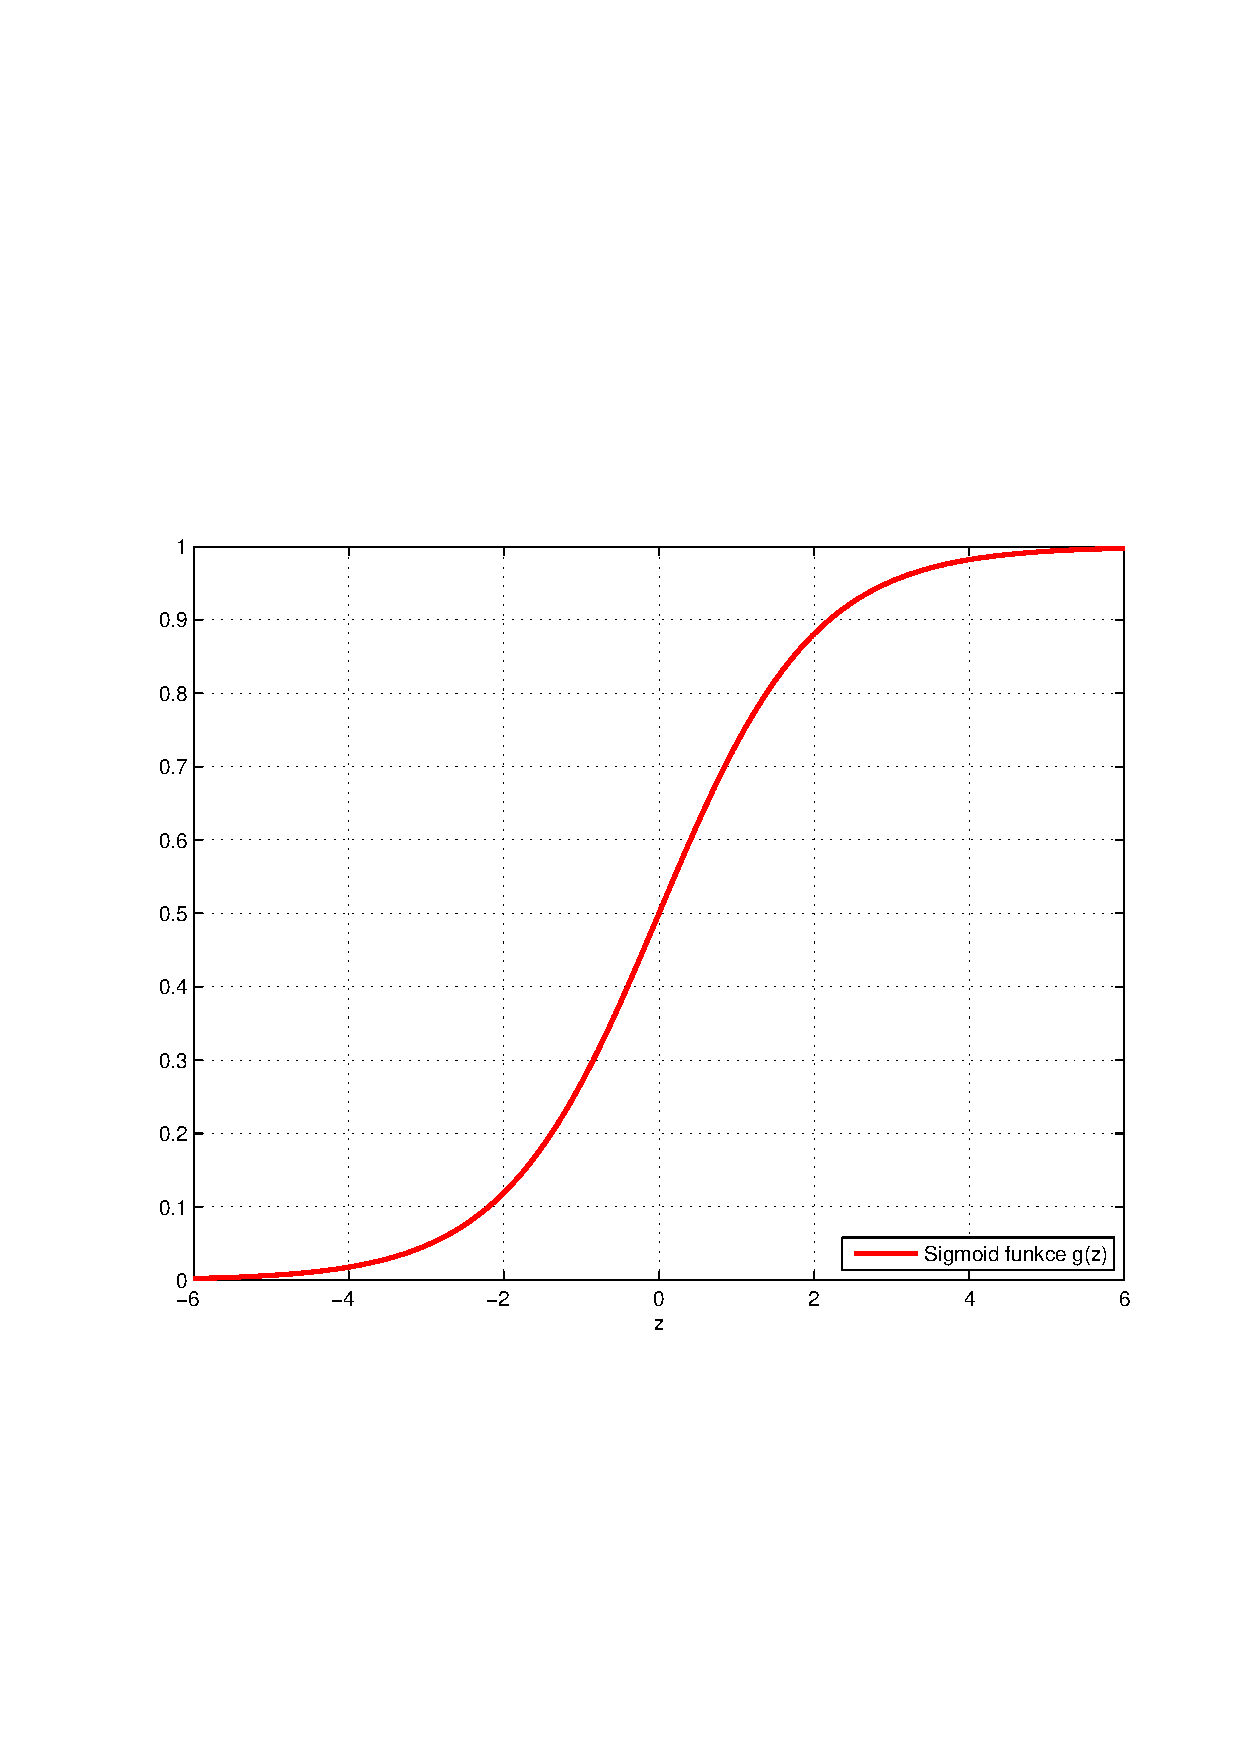
\includegraphics[width = 0.48\textwidth, trim = 2.5cm 7cm 2cm 9cm]{./Img/BinarniRegrese/sigmoidFunkce/sigmoidFunction.pdf}
	\caption{Sigmoidní funkce $g \left( z \right)$.}
	\label{fig:sigmoidFunction2}
\end{figure}}

\par{Podrobněji vysvětlíme, kdy naše hypotéza bude predikovat na výstupu 0 nebo 1. Konkrétně naše hypotéza bude na výstupu predikovat $y = 1$ v případě
\begin{equation}
	h_{\bm{\Theta}} \left( \bm{x} \right) = g \left( \bm{\Theta}^{\top} \bm{x} \right) = P \left( y = 1 | \bm{x}; \bm{\Theta} \right).
\end{equation}
Předpokládejme, že klasifikátor predikuje výstup $y = 1$ pokud $h_{\bm{\Theta}} \left( \bm{x} \right) \geq 0.5$, což platí pro $\bm{\Theta}^{\top} \bm{x} \geq 0$ a~klasifikátor predikuje výstup $y = 0$ pokud $h_{\bm{\Theta}} \left( \bm{x} \right) < 0.5$, což platí pro $\bm{\Theta}^{\top} \bm{x} < 0$.}

\newpage

\subsubsection*{Příklad - lineárně separabilní třídy}
\par{Předpokládejme, že máme trénovací sadu, která je znázorněna na Obr.~\ref{fig:decisionBoundary1} a~naše hypotéza má tvar
\begin{equation}
	h_{\bm{\Theta}} \left( \bm{x} \right) = g \left( \vartheta_0 + \vartheta_1 x_1 + \vartheta_2 x_2 \right).
	\label{eq:linearniHypotezaRovnice}
\end{equation}
Nyní se nebudeme zabývat tím, jak přizpůsobit parametry tomuto modelu. Předpokládejme, že $\bm{\Theta} = \left[ \vartheta_0,~\vartheta_1,~\vartheta2 \right]^{\top} = \left[ -3,~1,~1 \right]^{\top}$.}
\begin{figure}[!ht]
	\centering
	\begin{minipage}[t]{0.48\textwidth}
		%trim option's parameter order: left bottom right top
		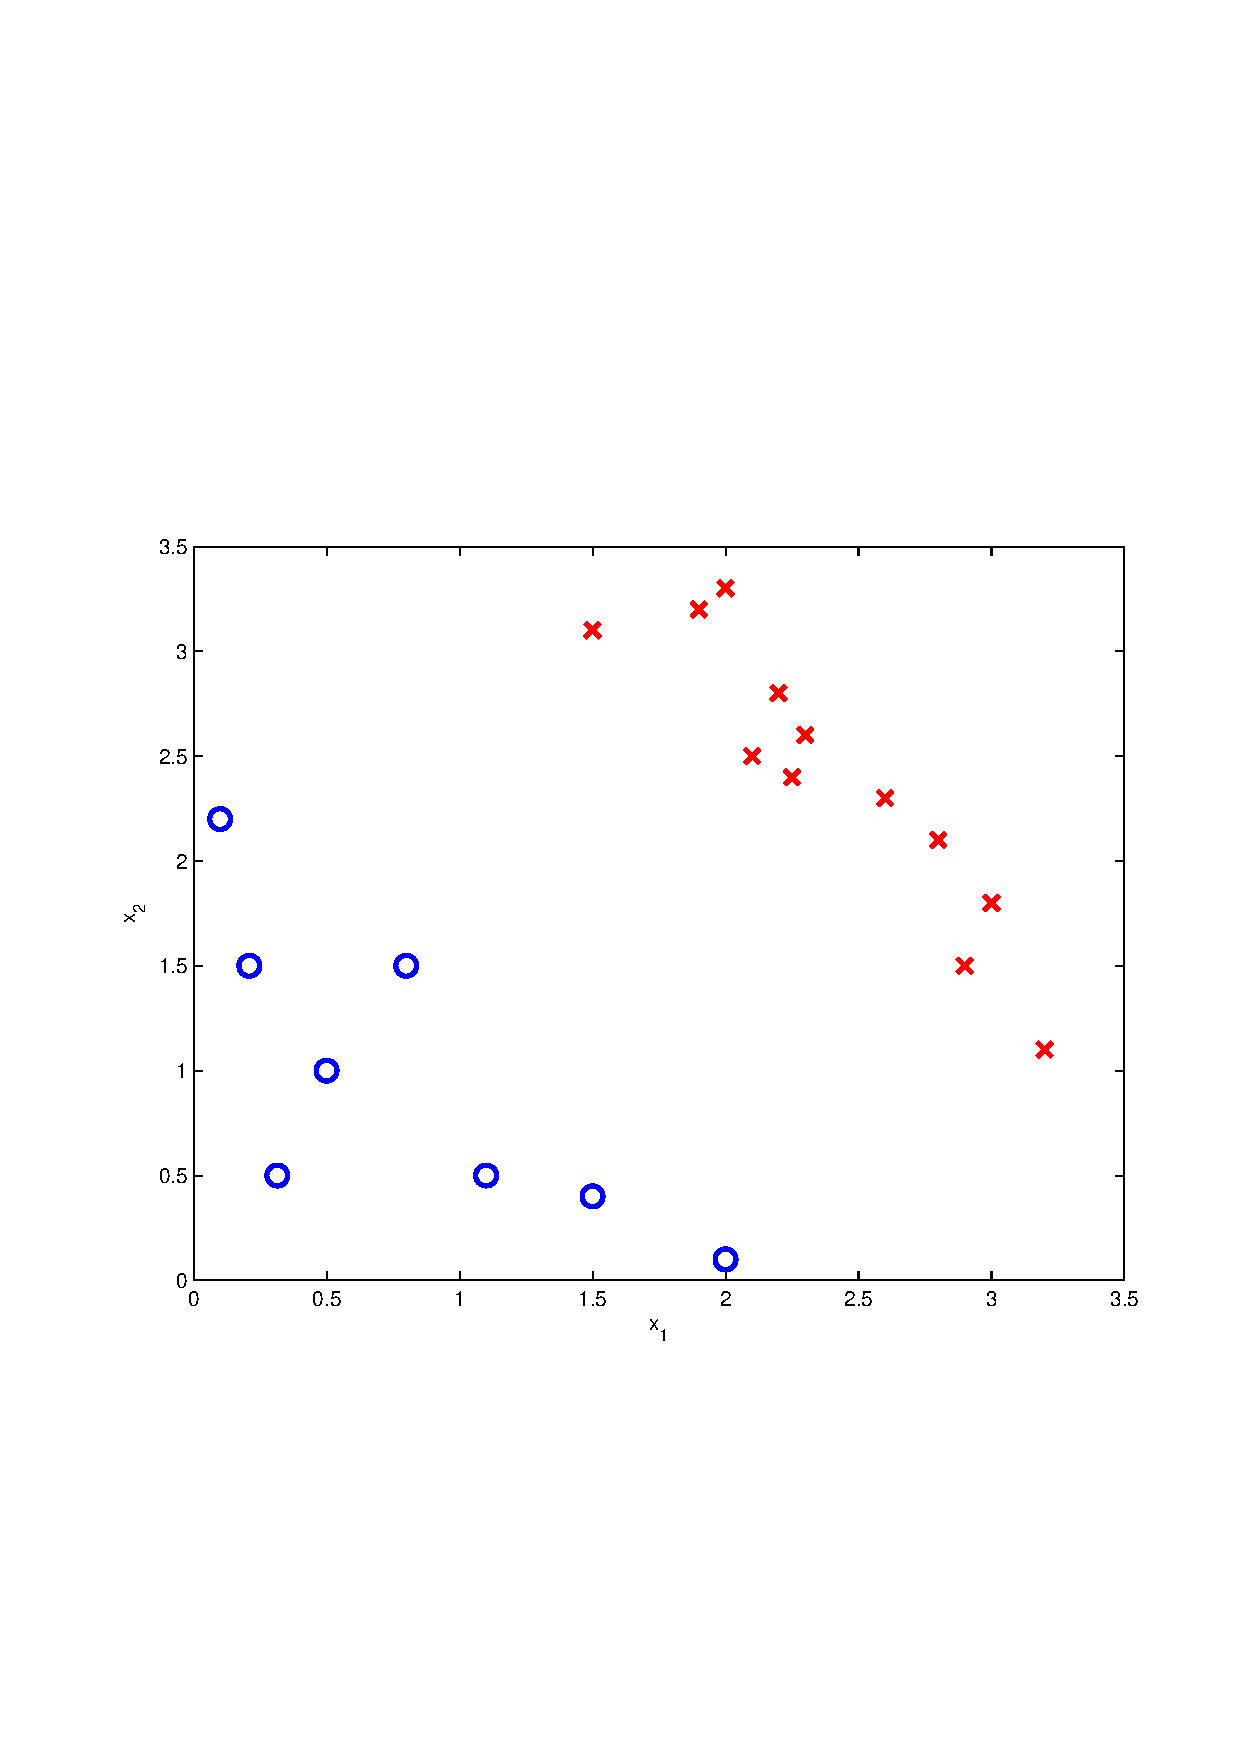
\includegraphics[width = \textwidth, trim = 2.5cm 7cm 2cm 9cm]{./Img/BinarniRegrese/decisionBoundary/decisionBoundary1.pdf}
		\caption{Vizualizace dvou tříd.}
		\label{fig:decisionBoundary1}
	\end{minipage}%
	\hfill
	\begin{minipage}[t]{0.48\textwidth}
		%trim option's parameter order: left bottom right top
		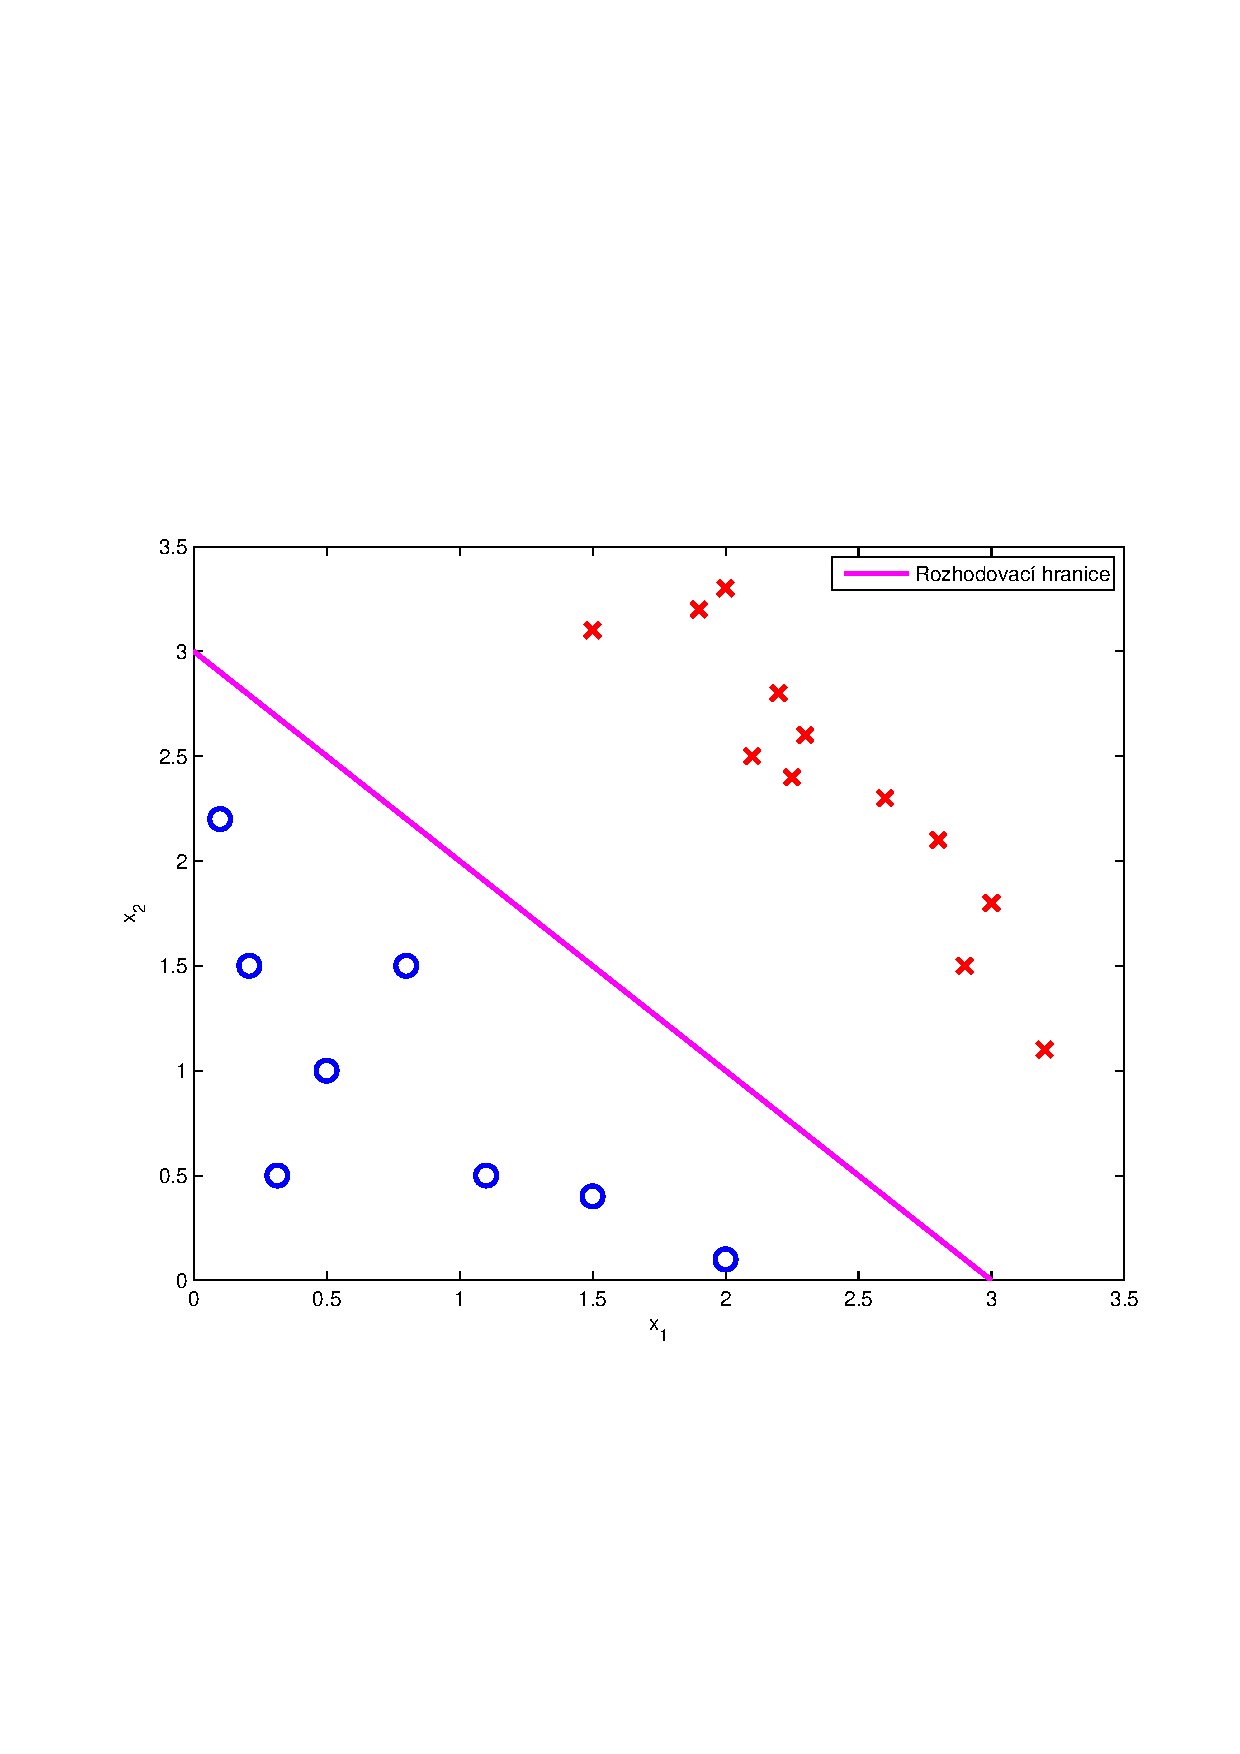
\includegraphics[width = \textwidth, trim = 2.5cm 7cm 2cm 9cm]{./Img/BinarniRegrese/decisionBoundary/decisionBoundary2.pdf}
		\caption{Vizualizace rozhodovací hranice.}
		\label{fig:decisionBoundary2}
	\end{minipage}%
\end{figure}

\par{Na příkladu si ukážeme, kdy hypotéza bude predikovat, jako výstup 0 a kdy 1. Hypotéza bude predikovat výstupní hodnotu $y = 1$ pokud
\begin{equation}
	-3 + x_1 + x_2 \geq 0
	\label{eq:prikladDecisionBoundary}
\end{equation}
($\bm{\Theta}^{\top} \bm{x} \geq 0$), jinými slovy pro všechna $x_1$ a $x_2$, které splňují rovnici \ref{eq:prikladDecisionBoundary} bude naše hypotéza predikovat výstup $y = 1$. Řešení rovnice \ref{eq:prikladDecisionBoundary} je naznačeno na Obr. \ref{fig:decisionBoundary2} a~odpovídají mu červené křížky nad rozhodovací hranicí.}

\par{V~případě, kdy $x_1 + x_2 = 3$, tak to odpovídá přesně $h_{\bm{\Theta}} \left( \bm{x} \right) = 0.5$. Jinak řečeno řešení odpovídá přesně rozhodovací hranici mezi třídami.}

\newpage

\subsubsection*{Příklad - lineárně neseparabilní třídy}
\par{Předpokládejme složitější příklad, kde nelze jednoduše použít binární regresi (lineární rozhodovací hranici) a~musíme využít polynomiální regrese, tedy musíme využít vyšší stupně polynomů jako příznaky viz Obr. \ref{fig:decisionBoundary3}.}
\begin{figure}[!ht]
	\centering
	\begin{minipage}[t]{0.48\textwidth}
		%trim option's parameter order: left bottom right top
		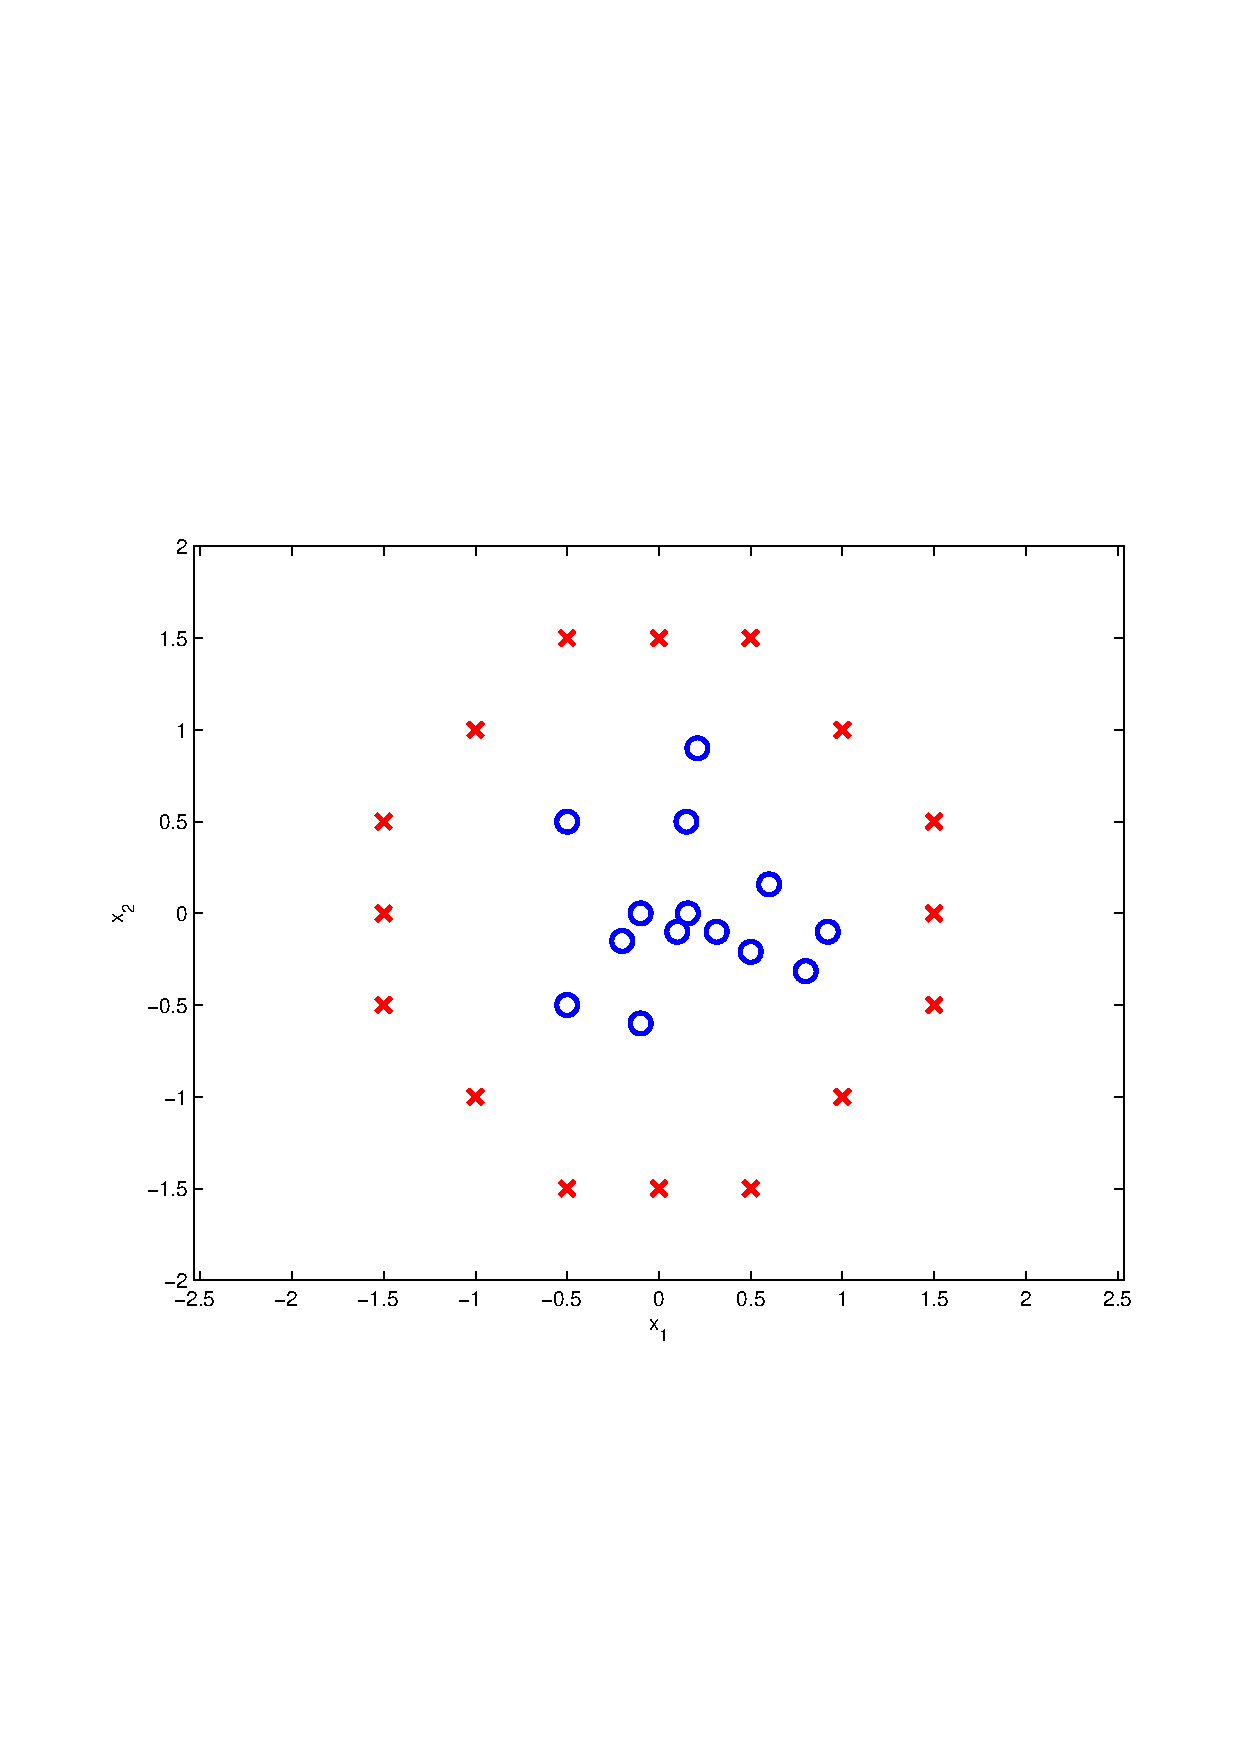
\includegraphics[width = \textwidth, trim = 2.5cm 7cm 2cm 9cm]{./Img/BinarniRegrese/decisionBoundary/decisionBoundary3.pdf}
		\caption{Vizualizace lineárně neseparabilních tříd.}
		\label{fig:decisionBoundary3}
	\end{minipage}%
	\hfill
	\begin{minipage}[t]{0.48\textwidth}
		%trim option's parameter order: left bottom right top
		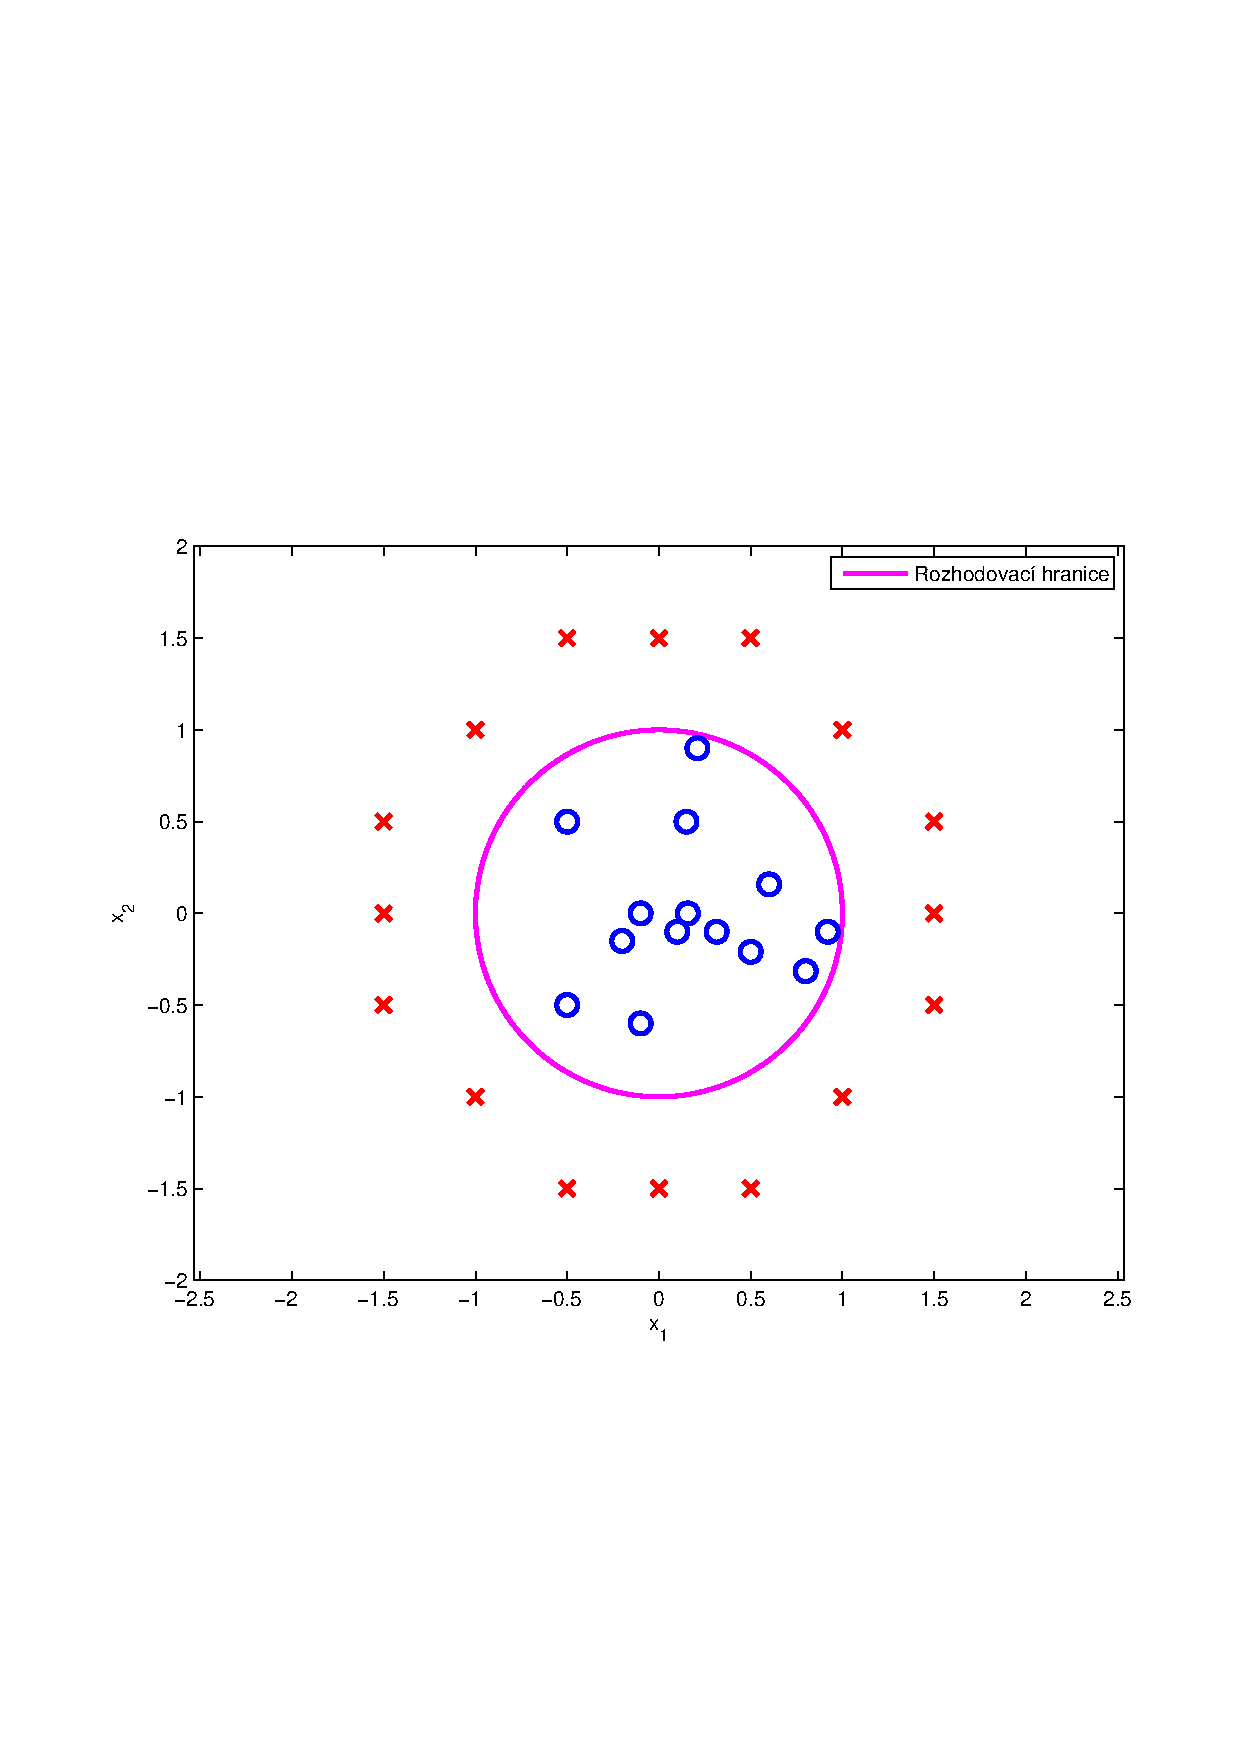
\includegraphics[width = \textwidth, trim = 2.5cm 7cm 2cm 9cm]{./Img/BinarniRegrese/decisionBoundary/decisionBoundary4.pdf}
		\caption{Vizualizace lineárně neseparabilních tříd společně s~rozhodovací hranicí.}
		\label{fig:decisionBoundary4}
	\end{minipage}%
\end{figure}

\par{Naše hypotéza má tvar $h_{\bm{\Theta}} \left( \bm{x} \right) = g \left( \vartheta_0 + \vartheta_1 x_1 + \vartheta_2 x_2 + \vartheta_3 x_1^2 + \vartheta_4 x_2^2 \right)$, kde jsme oproti předcházejícímu příkladu (rovnice \ref{eq:linearniHypotezaRovnice}) přidali dva příznaky $x_1^2$ a $x_2^2$ a~máme 5~parametrů $\vartheta_{0,\ldots,4}$. Nebudeme zabývat tím, jak vypočítat parametry $\bm{\Theta}$ (bude popsáno v~následujících sekcích), řekněme, že $\bm{\Theta} = \left[ \vartheta_0,~\vartheta_1,~\vartheta_2,~\vartheta_3,~\vartheta_4 \right]^{\top} = \left[ -1,~0,~0,~1,~1 \right]^{\top}$. Což znamená, že naše hypotéza bude predikovat výstup $y = 1$ pokud $-1 + x_1^2 + x_2^2 \geq 0$ (pro směr ven od rozhodovací hranice), tato rovnice odpovídá rovnici kružnice $x_1^2 + x_2^2 = 1$ o~poloměru $r = 1$. Rozhodovací hranice je vidět na Obr.~\ref{fig:decisionBoundary4}.}

\subsubsection*{Poznámka}
\par{Rozhodovací hranice je vlastnost hypotézy, konkrétně parametrů $\bm{\Theta}$, není to vlastnost trénovací sady. Trénovací sada je pouze využita k nalezení parametrů hypotézy~$\bm{\Theta}$.}





\newpage















%----------------------------------------------------------------------------------------
\subsection{Ztrátová funkce}
\label{sec:BinarniRegreseZtratovaFunkce}

\par{V této sekci si povíme jak vypočítat parametry $\bm{\Theta}$ pro binární regresi / klasifikaci.}

\par{Definujme problém učení s učitelem pro binární regresní model. Mějme trénovací množinu
\begin{equation}
	\{ \left( \bm{x}^{\left( 1 \right)}, y^{\left( 1 \right)} \right), \left( \bm{x}^{\left( 2 \right)}, y^{\left( 2 \right)} \right), \ldots , \left( \bm{x}^{\left( m \right)}, y^{\left( m \right)} \right) \}
\end{equation}
o velikosti $m$ vzorků, kde
\begin{equation}
	\bm{x}^{\left( i \right)} = \left[ x_0,~x_1,~\ldots,~x_n \right]^{\top},
\end{equation}
$\bm{x}^{\left( i \right)} \in \mathrm{R}^{n+1}$ a $x_0 = 1$, $y \in \{ 0,1 \}$. Naše hypotéza má tvar
\begin{equation}
	h_{\bm{\Theta}} \left( \bm{x} \right) = \frac{1}{1 + e^{-\bm{\Theta}^{\top} \bm{x}}}.
\end{equation}}

\par{Nyní si položme zásadní otázku, jak zvolit parametry $\bm{\Theta}$ v závislosti na naší trénovací množině?}

\par{Připomeňme si ztrátovou funkci $J \left( \bm{\Theta} \right)$ pro lineární regresi (viz sekce \ref{sec:LinearniRegreseZtratovaFunkce}), kterou zapíšeme v následujícím tvaru
\begin{equation}
	J \left( \bm{\Theta} \right) = \frac{1}{m} \sum_{i=1}^{m} \frac{1}{2} \left( h_{\Theta} \left( \bm{x}^{\left( i \right)} \right) - y^{\left( i \right)} \right)^2,
\end{equation}
dále můžeme ztrátovou funkci přepsat do tvaru
\begin{equation}
	J \left( \bm{\Theta} \right) = \frac{1}{m} \sum_{i=1}^{m} Cena \left( h_{\bm{\Theta}} \left( \bm{x}^{\left( i \right)} \right), y^{\left( i \right)} \right),
	\label{eq:JcenaX}
\end{equation}
kde
\begin{equation}
	Cena \left( h_{\bm{\Theta}} \left( \bm{x}^{\left( i \right)} \right), y^{\left( i \right)} \right) = \frac{1}{2} \left( h_{\bm{\Theta}} \left( \bm{x}^{\left( i \right)} \right) - y^{\left( i \right)} \right)^2.
	\label{eq:cenaX}	
\end{equation}
Nyní lze z rovnice \ref{eq:JcenaX} lépe vidět, že ztrátová funkce je $\frac{1}{m}$ krát součet $Cen$ přes trénovací sadu. Rovnici \ref{eq:cenaX} lze dále zjednodušit vynecháním horních indexů
\begin{equation}
	Cena \left( h_{\bm{\Theta}} \left( \bm{x} \right), y \right) = \frac{1}{2} \left( h_{\Theta} \left( \bm{x} \right) - y \right)^2
\end{equation}
a říká nám jakou $Cenu$ zaplatíme pokud výstupní hodnota hypotézy bude $h_{\bm{\Theta}} \left( \bm{x} \right)$ a výstupní informace od učitele bude hodnota $y$.}

\par{Tento předpis \ref{eq:cenaX} pro výpočet $Ceny$ platí pro lineární regresi. Avšak v této sekci se zajímáme o binární regresi. Pokud bychom chtěli minimalizovat tuto ztrátovou funkci v rovnici \ref{eq:JcenaX}, tak tato funkce může být nekonvexní vzhledem k parametrům $\bm{\Theta}$ (není zaručeno, že dosáhneme globálního minima, jako v případě konvexní ztrátové funkce).}

\par{Uveďme si ztrátovou funkci, která se využívá při binární regresi
\begin{equation}
	\label{eq:ztratovaFunkceBinarniRegrese}
	Cena \left( h_{\bm{\Theta}} \left( \bm{x} \right), y \right) = \left\{
	\begin{array}{r}
		{- \log \left( h_{\bm{\Theta}} \left( \bm{x} \right) \right), \quad \textrm{pro}~y = 1} \\
		{- \log \left( 1 - h_{\bm{\Theta}} \left( \bm{x} \right) \right), \quad \textrm{pro}~y = 0}
	\end{array}
	\right.
\end{equation}
jinými slovy lze říci, že se jedná jakou ztrátu (kolik nás stojí) utrpíme pokud $y = 0$ nebo $y = 1$.}


\newpage

\par{Nyní si ztrátovou funkci pro binární regresi, z rovnice \ref{eq:ztratovaFunkceBinarniRegrese}, rozebereme podrobněji. Na Obr. \ref{fig:ztratovaFunkce3} lze vidět průběh ztrátové funkce.
\begin{figure}[!ht]
	\centering
	%trim option's parameter order: left bottom right top
	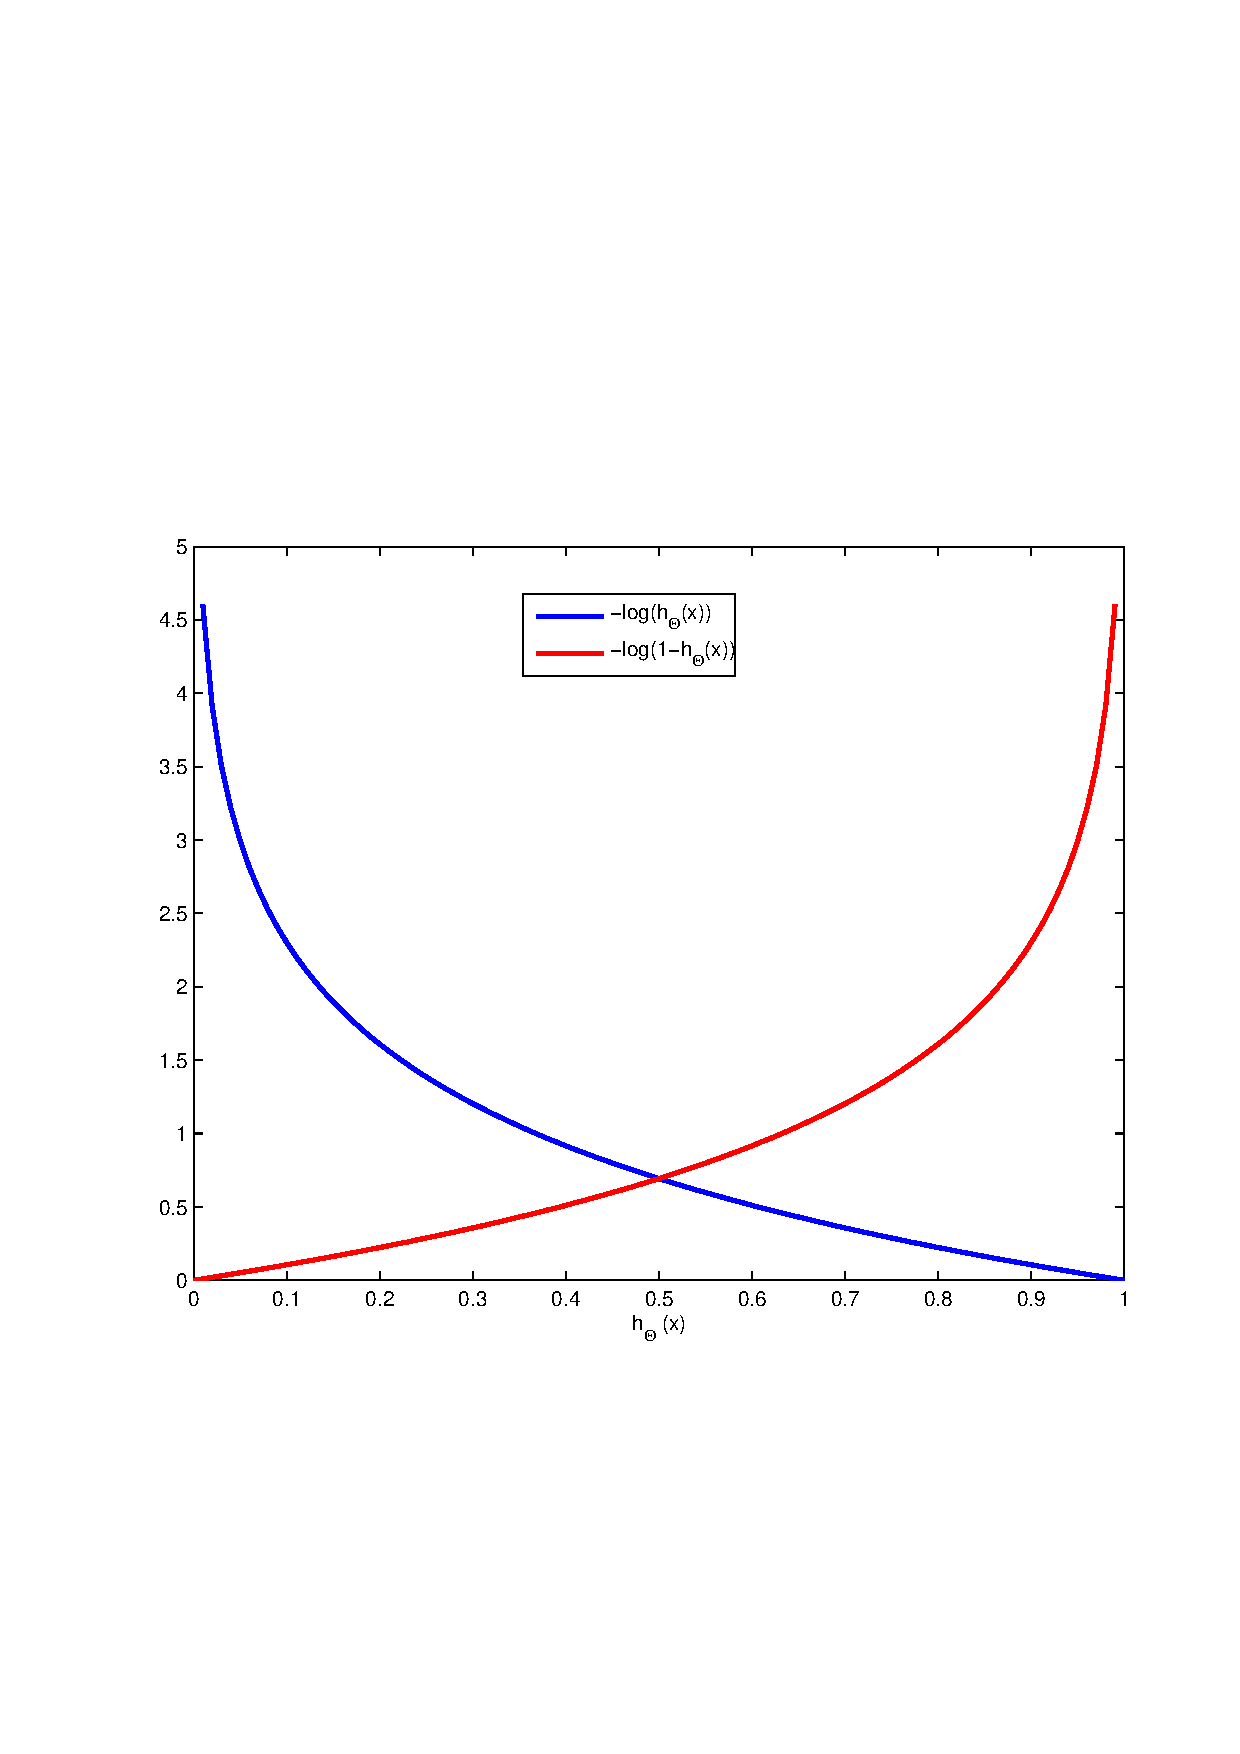
\includegraphics[width = 0.48\textwidth, trim = 2.5cm 7cm 2cm 9cm]{./Img/BinarniRegrese/ztratovaFunkce/ztratovaFunkce3.pdf}
	\caption{Průběh ztrátové funkce.}
	\label{fig:ztratovaFunkce3}
\end{figure}}

\par{Pokud bude $y = 1$ a naše hypotéza $h_{\bm{\Theta}} \left( \bm{x} \right) = 1$, tak utrpíme ztrátu rovnu $Cena = 0$. Ale pokud se bude hodnota hypotézy zmenšovat $h_{\bm{\Theta}} \left( \bm{x} \right) \rightarrow 0$, tak se utrpěná ztráta bude zvětšovat $Cena \rightarrow \infty$. V druhém případě pokud $h_{\bm{\Theta}} \left( \bm{x} \right) = 0$ (predikce $P \left( y = 1 | \bm{x}; \bm{\Theta} \right) = 0$), ale $y = 1$, tak utrpěná ztráta bude velmi velká.}

\par{Pro $y = 0$ platí obdobně druhá část rovnice \ref{eq:ztratovaFunkceBinarniRegrese}.}





















%----------------------------------------------------------------------------------------
\subsection{Zjednodušená ztrátová funkce a gradientní metoda}

\par{Naše ztrátová funkce $J \left( \bm{\Theta} \right)$ ve tvaru
\begin{equation}
	J \left( \bm{\Theta} \right) = \frac{1}{m} \sum_{i=1}^{m} Cena \left( h_{\bm{\Theta}} \left( \bm{x}^{\left( i \right)} \right), y^{\left( i \right)} \right),
	\label{eq:JcenaXpodruhe}
\end{equation}
kde
\begin{equation}
	\label{eq:ztratovaFunkceBinarniRegrese2}
	Cena \left( h_{\bm{\Theta}} \left( \bm{x} \right), y \right) = \left\{
	\begin{array}{r}
		{- \log \left( h_{\bm{\Theta}} \left( \bm{x} \right) \right), \quad \textrm{pro}~y = 1} \\
		{- \log \left( 1 - h_{\bm{\Theta}} \left( \bm{x} \right) \right), \quad \textrm{pro}~y = 0}
	\end{array}
	\right.
\end{equation}
poznamenejme že $y = 0$ nebo $y = 1$ (pokaždé, žádná jiná možnost není).}

\par{Naší $Cenu$ z rovnice \ref{eq:ztratovaFunkceBinarniRegrese2} můžeme zapsat v jedné rovnici, která má tvar
\begin{equation}
	Cena \left( h_{\bm{\Theta}} \left( \bm{x} \right), y \right) = - y \log \left( h_{\bm{\Theta}} \left( \bm{x} \right) \right) - \left( 1 - y \right) \log \left( 1 - h_{\bm{\Theta}} \left( \bm{x} \right) \right),
	\label{eq:cena1rovnice}
\end{equation}
pokud $y = 1$, tak rovnice \ref{eq:cena1rovnice} přechází na první část rovnice \ref{eq:ztratovaFunkceBinarniRegrese2} a pokud $y = 0$, tak rovnice \ref{eq:cena1rovnice} přechází na druhou část rovnice \ref{eq:ztratovaFunkceBinarniRegrese2}.}

\par{Po spojení a úpravě rovnic \ref{eq:cena1rovnice} a \ref{eq:JcenaXpodruhe} získáme výsledný tvar
\begin{equation}
		J \left( \bm{\Theta} \right) = - \frac{1}{m} \left[ \sum_{i=1}^{m} y^{\left( i \right)} \log \left( h_{\bm{\Theta}} \left( \bm{x}^{\left( i \right)} \right) \right) + \left( 1 - y^{\left( i \right)} \right) \log \left( 1 - h_{\bm{\Theta}} \left( \bm{x}^{\left( i \right)} \right) \right) \right].
		\label{eq:ztratovaFunkceJbinarniRegrese}
\end{equation}}

\par{Cílem je nalézt takové parametry $\bm{\Theta}$, které minimalizují ztrátovou funkci $J$
\begin{equation}
	\min_{\bm{\Theta}} J \left( \bm{\Theta} \right),
\end{equation}
a následně pro vypočítáme predikci naší hypotézy (na základě nového vstupu $x$) 
\begin{equation}
	h_{\bm{\Theta}} \left( \bm{x} \right) = \frac{1}{1 + e^{ - \bm{\Theta}^{\top} \bm{x}}}.
\end{equation}}

\par{Nyní můžeme konečně zapsat celý gradientní algoritmus, opakuj
\begin{equation}
	\vartheta_j = \vartheta_j - \alpha \frac{\partial}{\partial \vartheta_j} J \left( \bm{\Theta} \right),
	\label{eq:gradientDescentBinaryRegresionAlgorithm}
\end{equation}
po každé iteraci aktualizuj všechny parametry $\vartheta_j$ najednou dokud algoritmus nedokonverguje.}

\subsubsection*{Poznámka}
\par{V rovnici \ref{eq:gradientDescentBinaryRegresionAlgorithm} bude využit tvar
\begin{equation}
	\frac{\partial}{\partial \vartheta_j} J \left( \bm{\Theta} \right) = \frac{1}{m} \sum_{i = 1}^{m} \left( h_{\bm{\Theta}} \left( \bm{x}^{\left( i \right)} \right) - y^{\left( i \right)} \right) \bm{x}_j^{\left( i \right)}.
\end{equation} a proto je výhodnější psát rovnici \ref{eq:gradientDescentBinaryRegresionAlgorithm} ve tvaru
\begin{equation}
		\vartheta_j = \vartheta_j - \alpha \sum_{i = 1}^{m} \left( h_{\bm{\Theta}} \left( \bm{x}^{\left( i \right)} \right) - y^{\left( i \right)} \right) \bm{x}_j^{\left( i \right)}.
\end{equation}}

\par{Algoritmus vypadá totožně jako v případě lineární regrese (viz \ref{eq:NDgradientDescentVysledna}) s rozdílnou hypotézou $h_{\bm{\Theta}} \left( \bm{x} \right)$, v případě lineární regrese
\begin{equation}
	h_{\bm{\Theta}} \left( \bm{x} \right) = \bm{\Theta}^{\top} \bm{x}
\end{equation}
a v případě binární regrese se jedná o
\begin{equation}
	h_{\bm{\Theta}} \left( \bm{x} \right) = \frac{1}{1 + e^{- \bm{\Theta}^{\top} \bm{x}}}.
\end{equation}}

\subsubsection*{Poznámka}
\par{Při výpočtu parametrů $\bm{\Theta}$ pomocí gradientního algoritmu v případě binární regrese je také vhodné využít Features scaling, jako v případě lineární regrese (viz sekce \ref{sec:featuresScaling}).}



\newpage



















%----------------------------------------------------------------------------------------
\subsection{Pokročilé algoritmy optimalizace}

\par{V této sekci si uvedeme příklady několika pokročilejších algoritmů optimalizace, které jsou lépe využitelné pro velké problémy strojového učení, kde je například velký počet příznaků.}

\par{Připomeňme náš optimalizační problém, máme ztrátovou funkci $J \left( \bm{\Theta} \right)$ a chceme jí minimalizovat
\begin{equation}
	\min_{\bm{\Theta}} J \left( \bm{\Theta} \right).
\end{equation}
Musíme tedy znát rovnice pro výpočet $J \left( \bm{\Theta} \right)$ a $\frac{\partial}{\partial \vartheta_j} J \left( \bm{\Theta} \right)$ následně můžeme využít zmíněný gradientní algoritmus, nebo nějakou z pokročilejších optimalizačních metod jako jsou například
\begin{table}[!ht]
\begin{center}
\begin{tabular}{r|c|c}
	{Název algoritmu} & {Výhody} & {Nevýhody}\\
	\hline
	{Conjugate gradient} & {Nemusí se volit} & {Více složité}\\
	{BFGS} & {konstanta učení $\alpha$.} & {}\\
	{L-BFGS} & {Rychlejší než gradientní metoda.} & {}
\end{tabular}
	\caption{Příklady pokročilejších optimalizačních algoritmů.}
\end{center}
\end{table}}

\subsubsection*{Příklad}
\par{Nyní si uvedeme příklad společně s jeho implementací v~MATLABu. Mějme vektor parametrů $\bm{\Theta} = \left[ \vartheta_1,~\vartheta_2 \right]^{\top}$ a ztrátovou funkci $J \left( \bm{\Theta} \right) = \left( \vartheta_1 - 5 \right)^2 + \left( \vartheta_2 - 5 \right)^2,$ dále vypočteme parciální derivace ztrátové funkce
\begin{eqnarray}
	\label{eq:prGrad1}
	\frac{\partial}{\partial \vartheta_1} &J \left( \bm{\Theta} \right) &= 2 \cdot \left( \vartheta_1 - 5 \right),\\
	\label{eq:prGrad2}
	\frac{\partial}{\partial \vartheta_2} &J \left( \bm{\Theta} \right) &= 2 \cdot \left( \vartheta_2 - 5 \right).
\end{eqnarray}}

\par{Program v~prostředí MATLAB by mohl vypadat následovně, nejprve je nutné si vytvořit funkci pro výpočet ztrátové funkce, která bude vracet hodnotu ztrátové funkce a~jednotlivé gradienty.
\lstinputlisting[language = Matlab]{./Img/BinarniRegrese/pokrocileOptimalizace/costFunction.m}}
\newpage


\par{Optimalizaci ztrátové funkce (hledání minima) můžeme spustit následovně.
\lstinputlisting[language = Matlab]{./Img/BinarniRegrese/pokrocileOptimalizace/run.m}
Výsledné hodnoty pro $\vartheta_{1,2} = 5$, což lze pro tento jednoduchý případ vidět z~rovnic \ref{eq:prGrad1}~a~\ref{eq:prGrad2}. Jak lze vidět z příkladu, nebylo nutné nastavovat parametr $\alpha$, funkce \textit{fminunc} v MATLABu si jej nastavila sama.}




\newpage














%----------------------------------------------------------------------------------------
\subsection{Klasifikace do více tříd}
\label{sec:BinarniRegreseKlasifikaceDoViceTrid}

\par{V této sekci si povíme o~klasifikaci do více tříd. Tento problém lze uchopit tak, že budeme klasifikovat jednu třídu proti všem ostatním, náš klasifikační algoritmus by se dal nazvat jeden proti všem.}

\par{Nejdříve si popišme náš klasifikační problém, lze ho demonstrovat na příkladu klasifikace emailů. Představme si, že bychom rádi příchozí emaily rozdělovali do složek, nebo označovali podle skupiny lidí, od kterých nám email přišel, například pracovní emaily, emaily od kamarádů, emaily od rodiny a emaily od známých, s~kterými sdílíme koníčky. Neboli chceme klasifikovat do tříd $y = \{ 1,~ 2,~ 3,~ 4 \}$. Na Obr. \ref{fig:oneVSall_one} a \ref{fig:oneVSall_all} je vidět rozdíl v~klasifikaci do dvou a více tříd.
\begin{figure}[!ht]
	\centering
	\begin{minipage}[b]{0.48\textwidth}
  		%trim option's parameter order: left bottom right top
		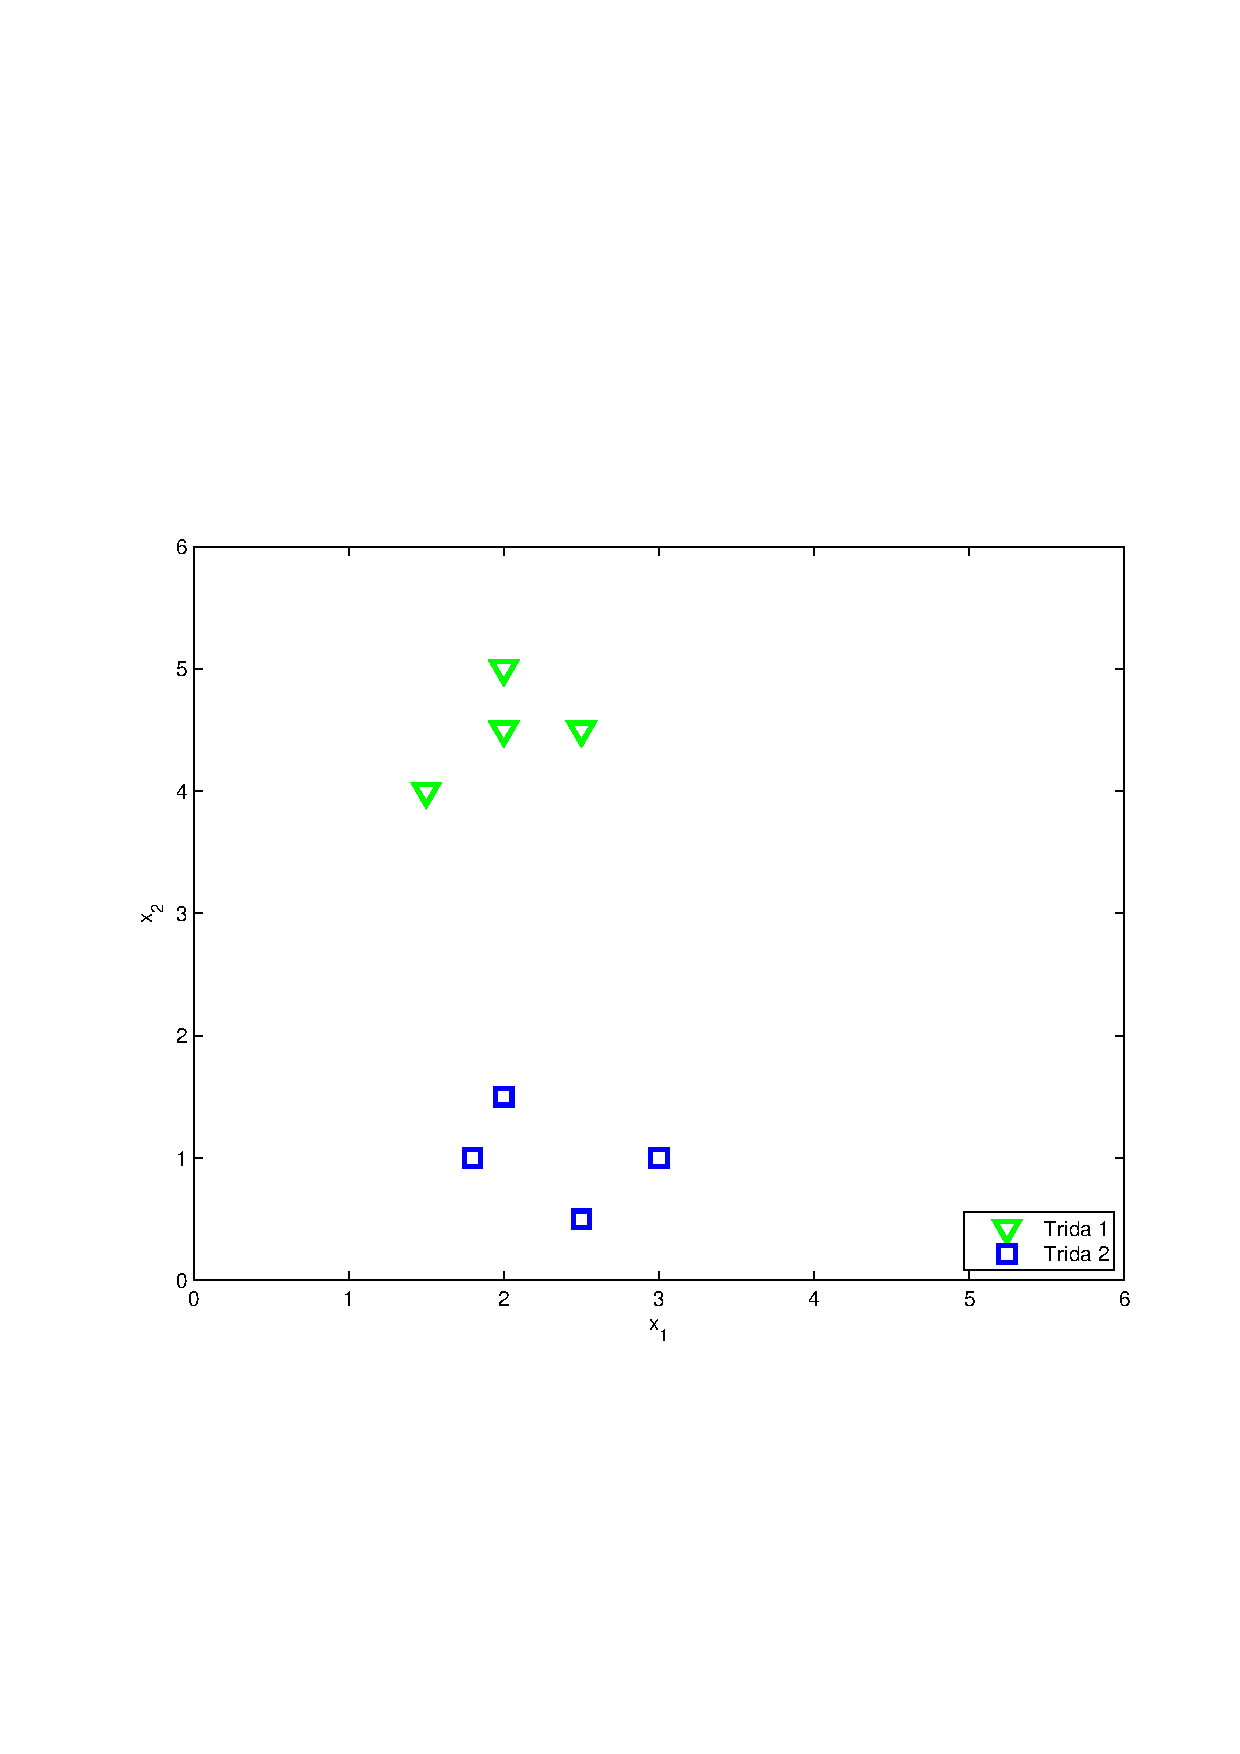
\includegraphics[width = \textwidth, trim = 2.5cm 7cm 2cm 9cm]{./Img/BinarniRegrese/oneVSallClassification/oneVSall_one.pdf}
  		\caption{Klasifikace do dvou tříd.}
		\label{fig:oneVSall_one}
	\end{minipage}%
	\hfill
	\begin{minipage}[b]{0.48\textwidth}
		%trim option's parameter order: left bottom right top
		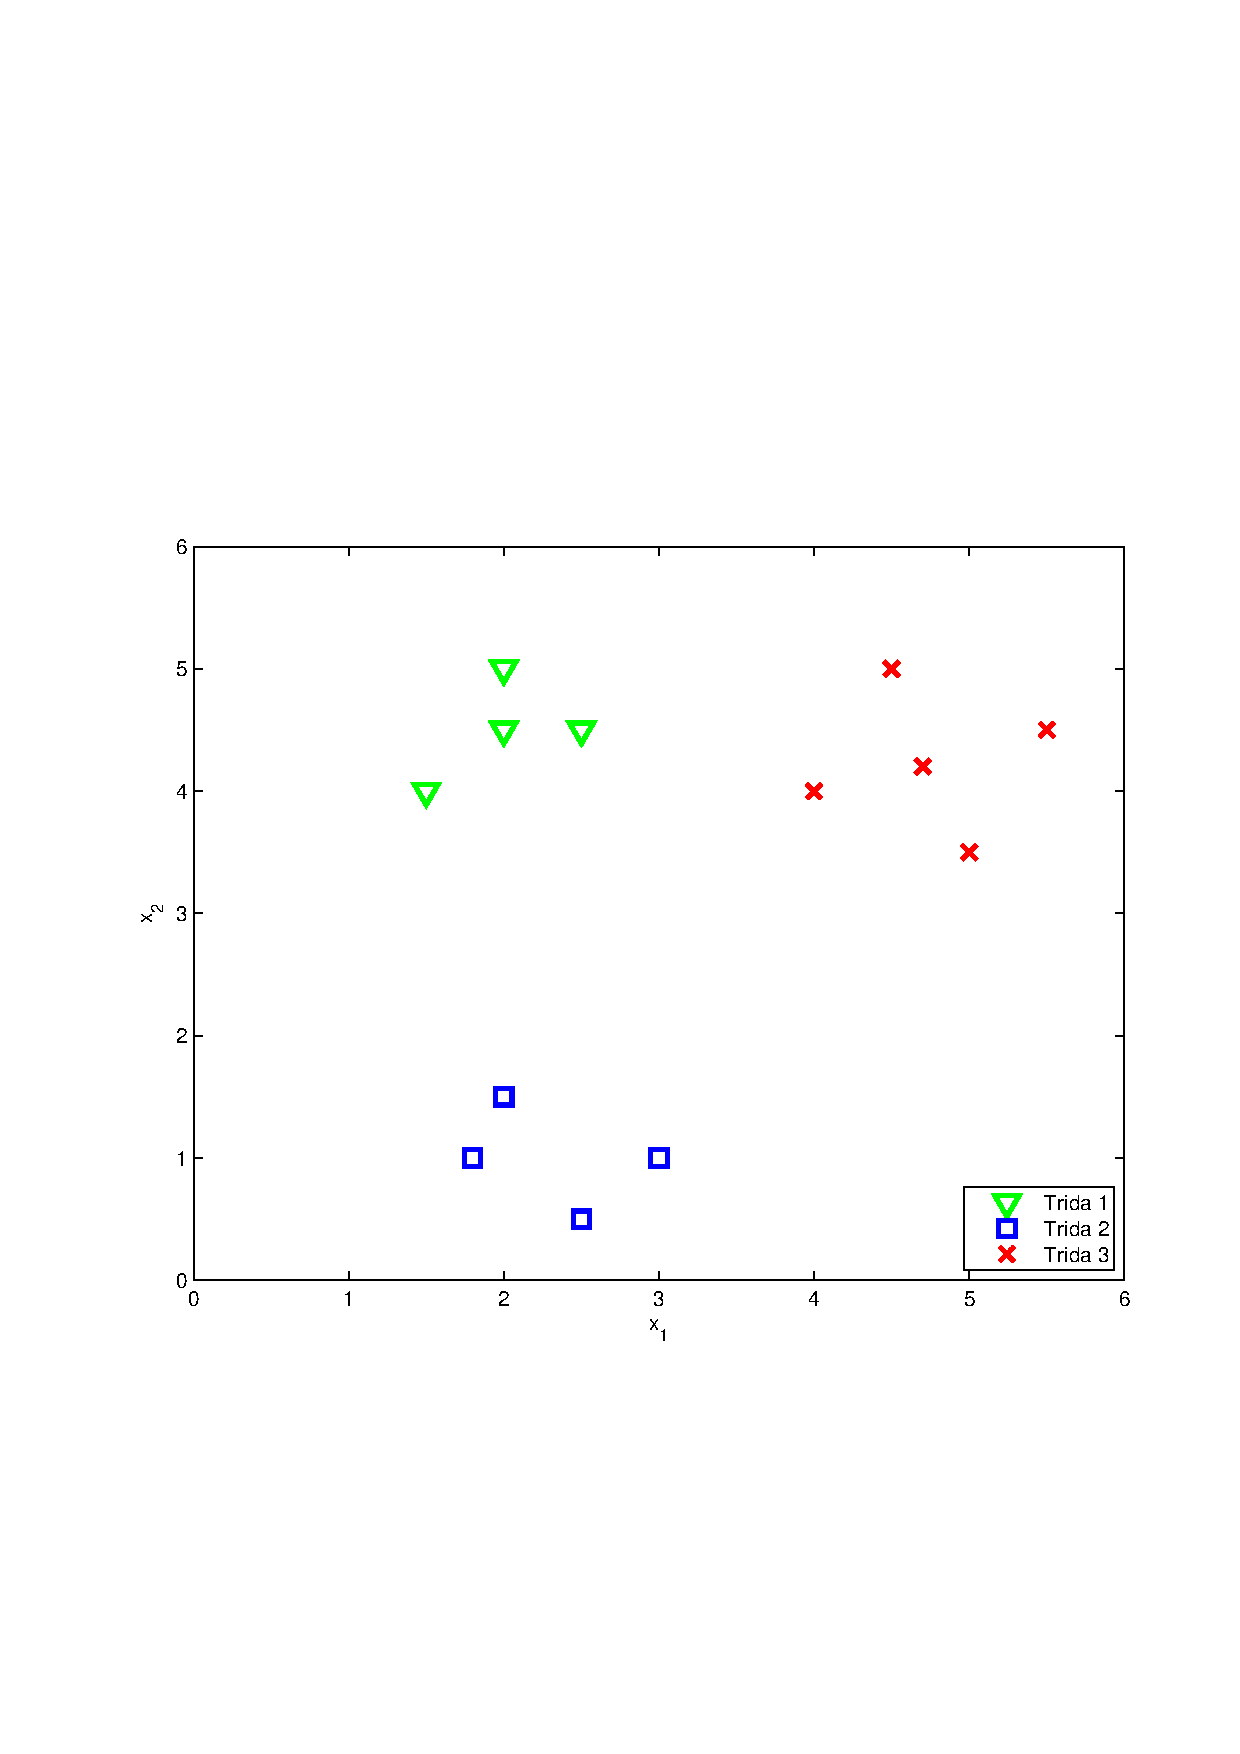
\includegraphics[width = \textwidth, trim = 2.5cm 7cm 2cm 9cm]{./Img/BinarniRegrese/oneVSallClassification/oneVSall_all.pdf}
  		\caption{Klasifikace do více tříd.}
		\label{fig:oneVSall_all}
	\end{minipage}%
\end{figure}}

\par{Z předešlých sekcí víme jak klasifikovat do dvou tříd. Nyní tento přístup použijeme při řešení problému klasifikace do více tříd. Na Obr. \ref{fig:oneVSall_all2} je znázorněno rozložení tříd a~následně na Obr.~\ref{fig:oneVSall_1} je ukázána klasifikace třídy~1 proti třídě, která je zkonstruována spojením všech ostatních tříd (v~našem případě tříd 2~a~3). Na dalších Obr.~\ref{fig:oneVSall_2} a~\ref{fig:oneVSall_3} jsou naznačeny zbylé kombinace.}Pro jednotlivé klasifikace je nutné vytvořit hypotézu
\begin{equation}
	h_{\bm{\Theta}}^{\left( i \right)} \left( \bm{x} \right), \quad i \in \{ 1,~2,~3\},
\end{equation}
která odpovídá pravděpodobnostem
\begin{equation}
	h_{\bm{\Theta}}^{\left( i \right)} \left( \bm{x} \right) = P \left( y = i| \bm{x} ; \bm{\Theta} \right).
\end{equation}}
\pagebreak

\begin{figure}[!ht]
	\centering
	\begin{minipage}[b]{0.48\textwidth}
  		%trim option's parameter order: left bottom right top
		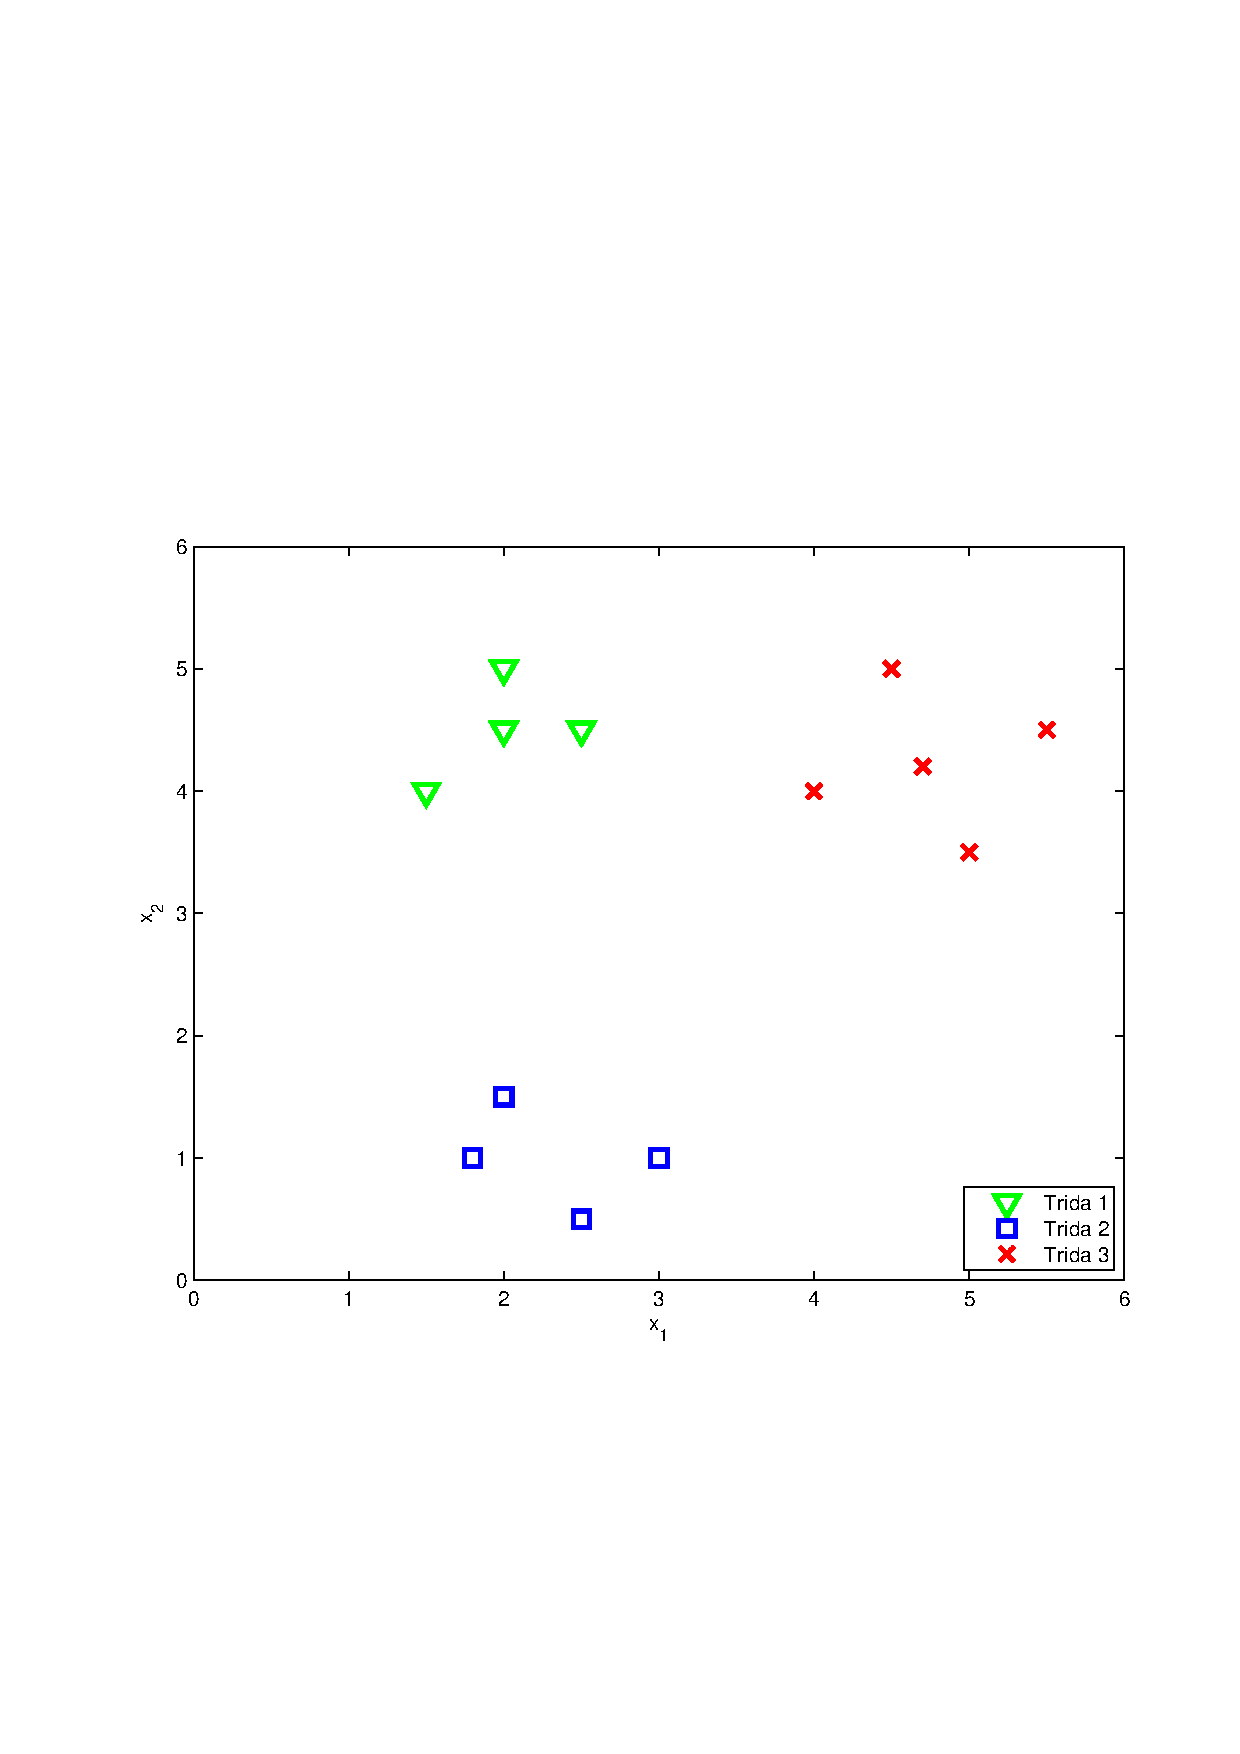
\includegraphics[width = \textwidth, trim = 2.5cm 7cm 2cm 9cm]{./Img/BinarniRegrese/oneVSallClassification/oneVSall_all.pdf}
  		\caption{Rozložení tříd $y = \{1,~2,~3\}$.}
		\label{fig:oneVSall_all2}
	\end{minipage}%
	\hfill
	\begin{minipage}[b]{0.48\textwidth}
		%trim option's parameter order: left bottom right top
		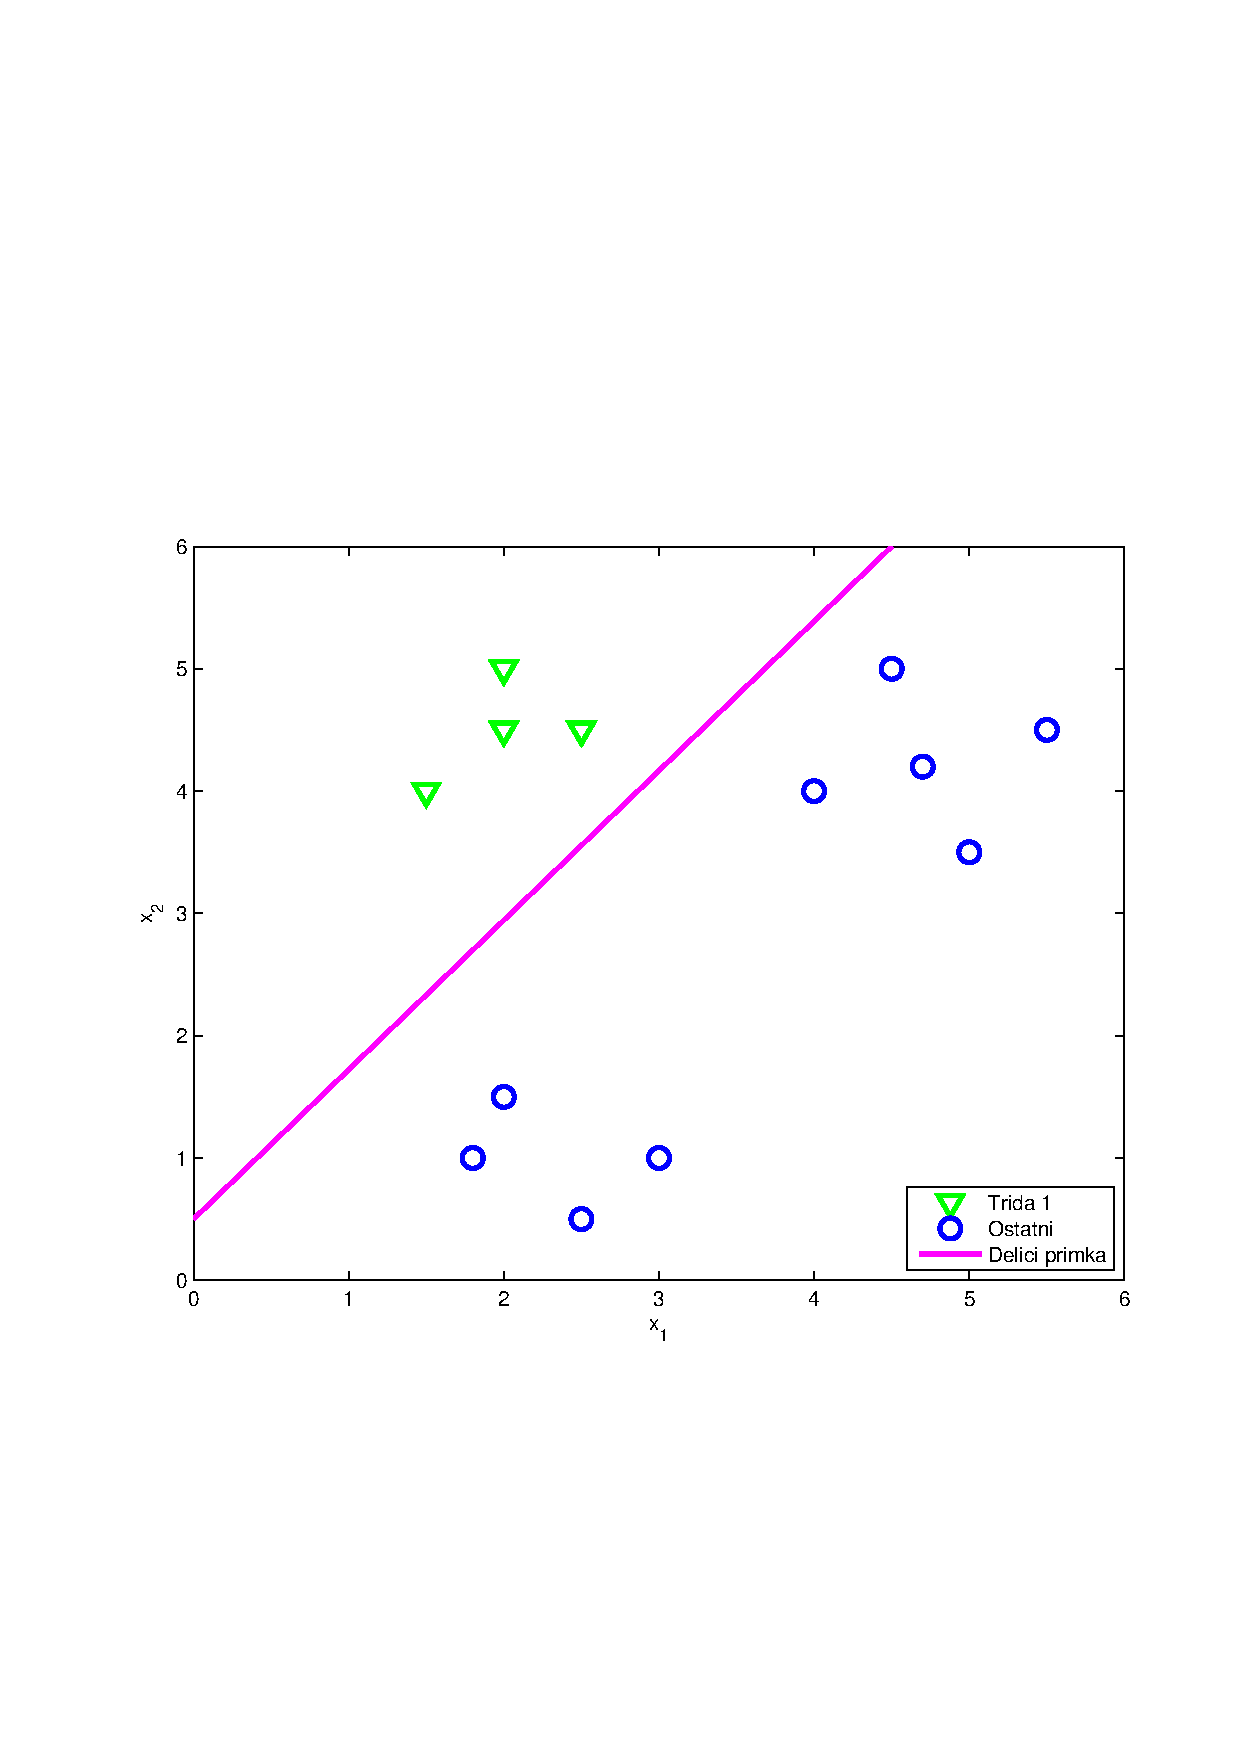
\includegraphics[width = \textwidth, trim = 2.5cm 7cm 2cm 9cm]{./Img/BinarniRegrese/oneVSallClassification/oneVSall_1.pdf}
  		\caption{Klasifikace třídy 1.}
		\label{fig:oneVSall_1}
	\end{minipage}%
\end{figure}
\begin{figure}[!ht]
	\centering
	\begin{minipage}[b]{0.48\textwidth}
  		%trim option's parameter order: left bottom right top
		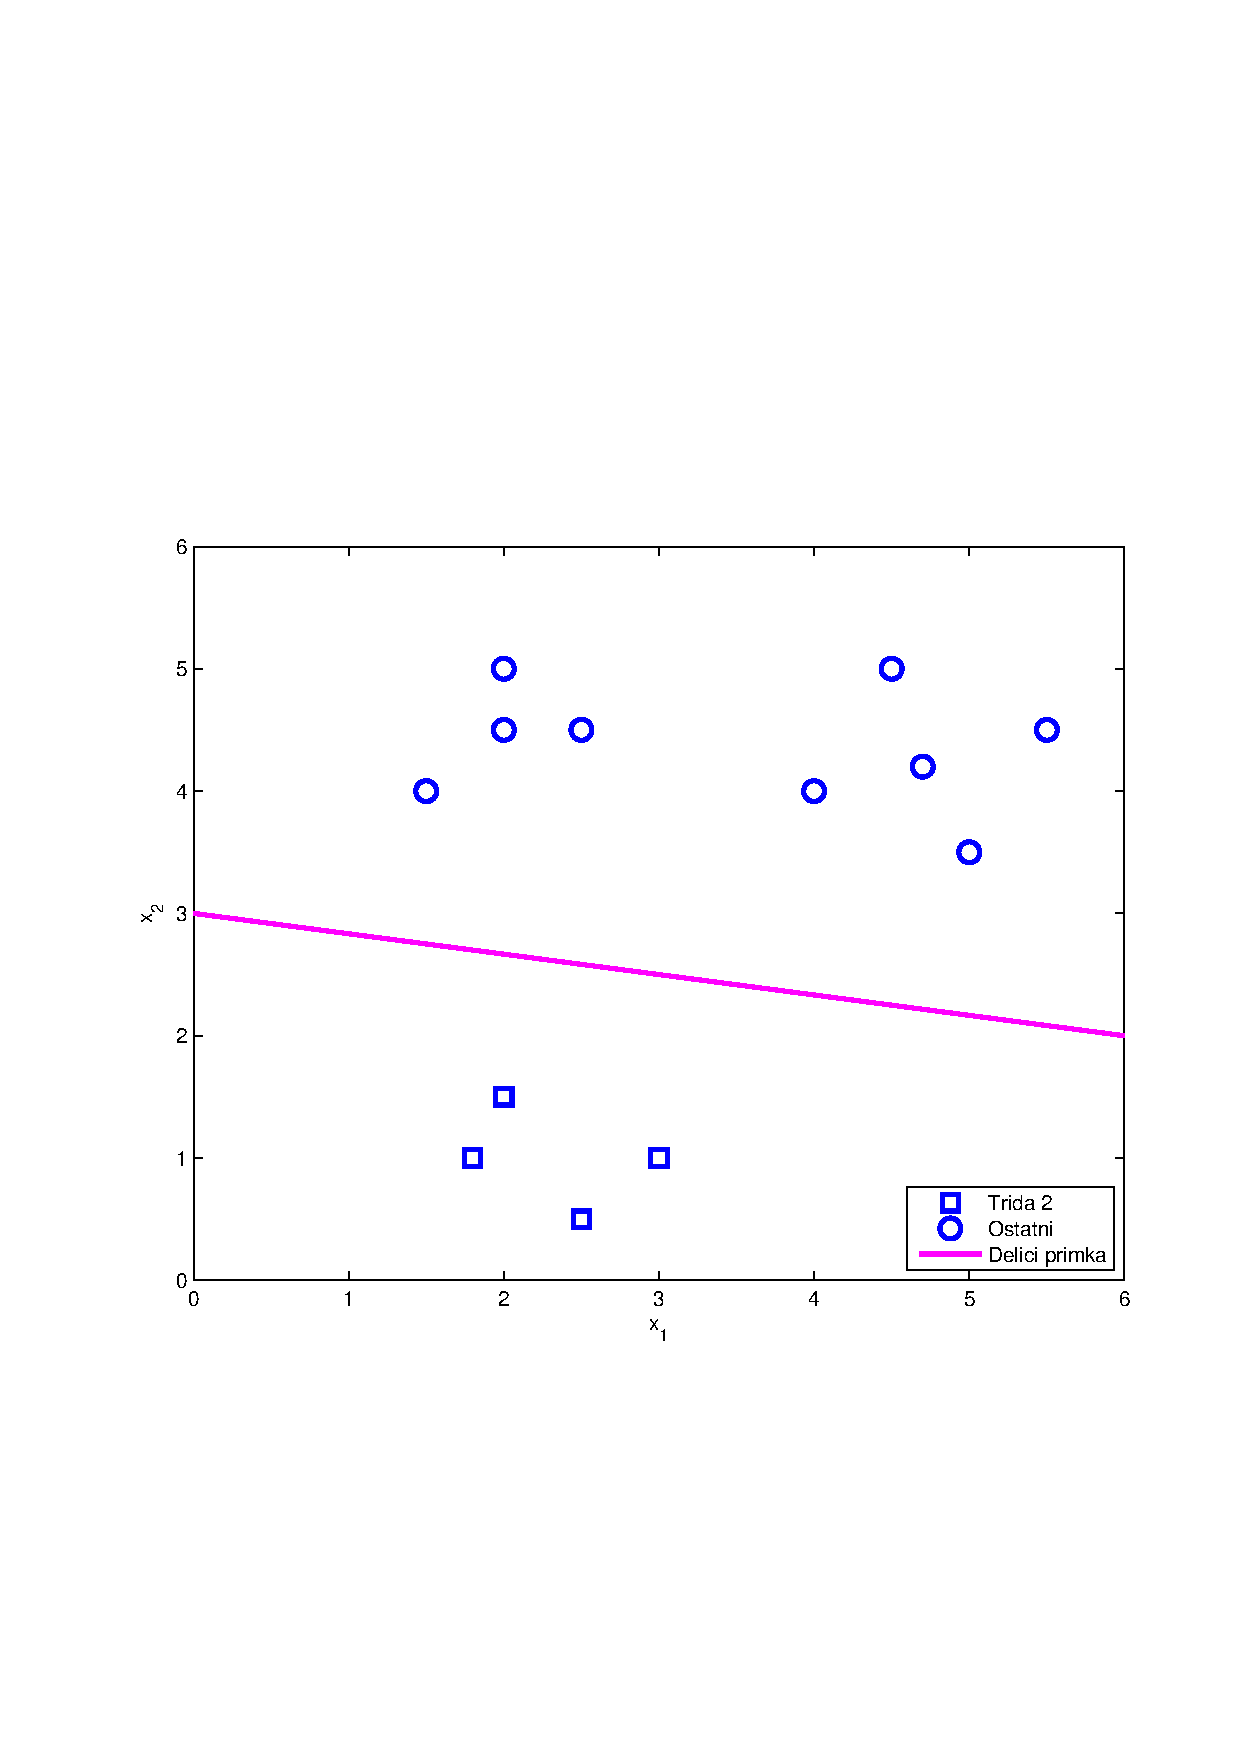
\includegraphics[width = \textwidth, trim = 2.5cm 7cm 2cm 9cm]{./Img/BinarniRegrese/oneVSallClassification/oneVSall_2.pdf}
  		\caption{Klasifikace třídy 2.}
		\label{fig:oneVSall_2}
	\end{minipage}%
	\hfill
	\begin{minipage}[b]{0.48\textwidth}
		%trim option's parameter order: left bottom right top
		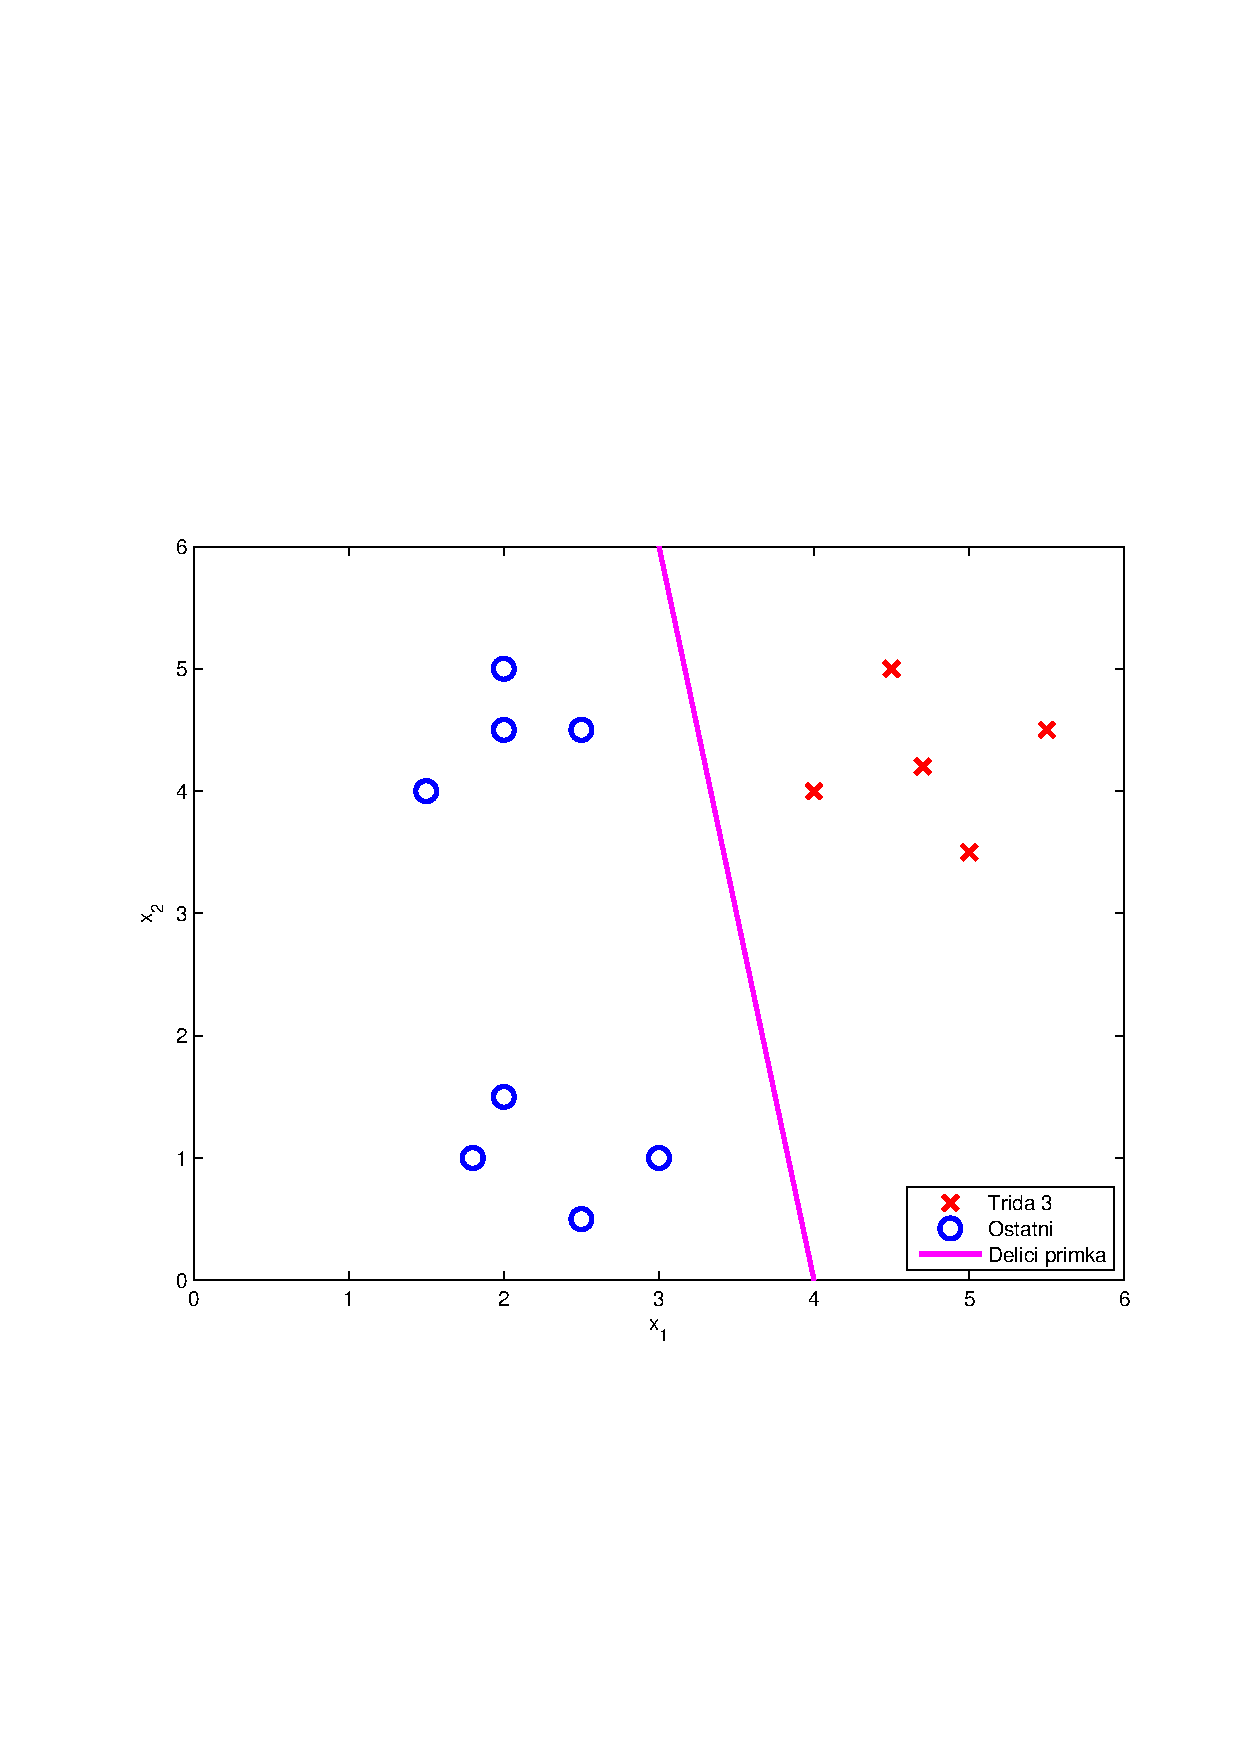
\includegraphics[width = \textwidth, trim = 2.5cm 7cm 2cm 9cm]{./Img/BinarniRegrese/oneVSallClassification/oneVSall_3.pdf}
  		\caption{Klasifikace třídy 3.}
		\label{fig:oneVSall_3}
	\end{minipage}%
\end{figure}

\subsubsection*{Shrnutí}
\par{Nejdříve je nutné natrénovat binární klasifikátory $h_{\bm{\Theta}}^{\left( i \right)} \left( \bm{x} \right)$ pro všechny třídy $i$ pro predikci pravděpodobnosti, že vzorek bude patřit do třídy $y = i$. Následně pro nový vstup $x$ klasifikovat podle všech hypotéz a vybrat takovou třídu $i$, která maximalizuje pravděpodobnost hypotézy
\begin{equation}
	 \max_{i} h_{\bm{\Theta}}^{\left( i \right)} \left( \bm{x} \right).
\end{equation}}


\newpage





















%----REGULARIZACE-----------------------------------------------------------------












%----REGULARIZACE------------------------------------------------------------------------------------
\section{Regularizace}
\label{sec:Regularizace}
















%----PROBLEM-PRETRENOVANI---------------------------------------------------------------------------
\subsection{Problém přetrénování}
\label{sec:RegularizaceProblemPretrenovani}

\par{Nyní když známe algoritmy lineární a binární regrese, které se hodí pro řešení mnoha úloh strojového učení, musíme si říci něco o problému zvaném přetrénování. Tento problém způsobuje, že dané algoritmy ve výsledku fungují velmi špatně.}

\par{V této sekci si vysvětlíme v čem problém přetrénování spočívá a v následujících sekcích bude popsán postup jak se s daným problémem vypořádat.}

\par{Vraťme se k našemu problému predikce ceny velikosti bytu, ve kterém jsme využili algoritmu lineární regrese.}

\par{Na Obr.~\ref{fig:regrese_0} jsou znázorněná trénovací data. Pokud využijeme lineární regresi společně s hypotézou $h_{\bm{\Theta}} \left( \bm{x} \right) = \vartheta_0 + \vartheta_1 x$, tak získáme predikci ve tvaru, který lze vidět na Obr. \ref{fig:regrese_1}. V tomto případě naše zvolená hypotéza $h_{\bm{\Theta}} \left( \bm{x} \right)$ nerespektuje dostatečně tvar našich trénovacích dat. Přesnější anglický termín pro takto nastalou situaci zní \textit{underfit} nebo \textit{high bias}, což se dá vysvětlit jako problém, kdy se snažíme použít regresi na trénovací data s~málo komplexní hypotézou. Tedy hypotéza nemůže dostatečně přesně vystihovat tvar dat (nezobecňuje).}
\begin{figure}[!ht]
	\centering
	\begin{minipage}[t]{0.48\textwidth}
  		%trim option's parameter order: left bottom right top
		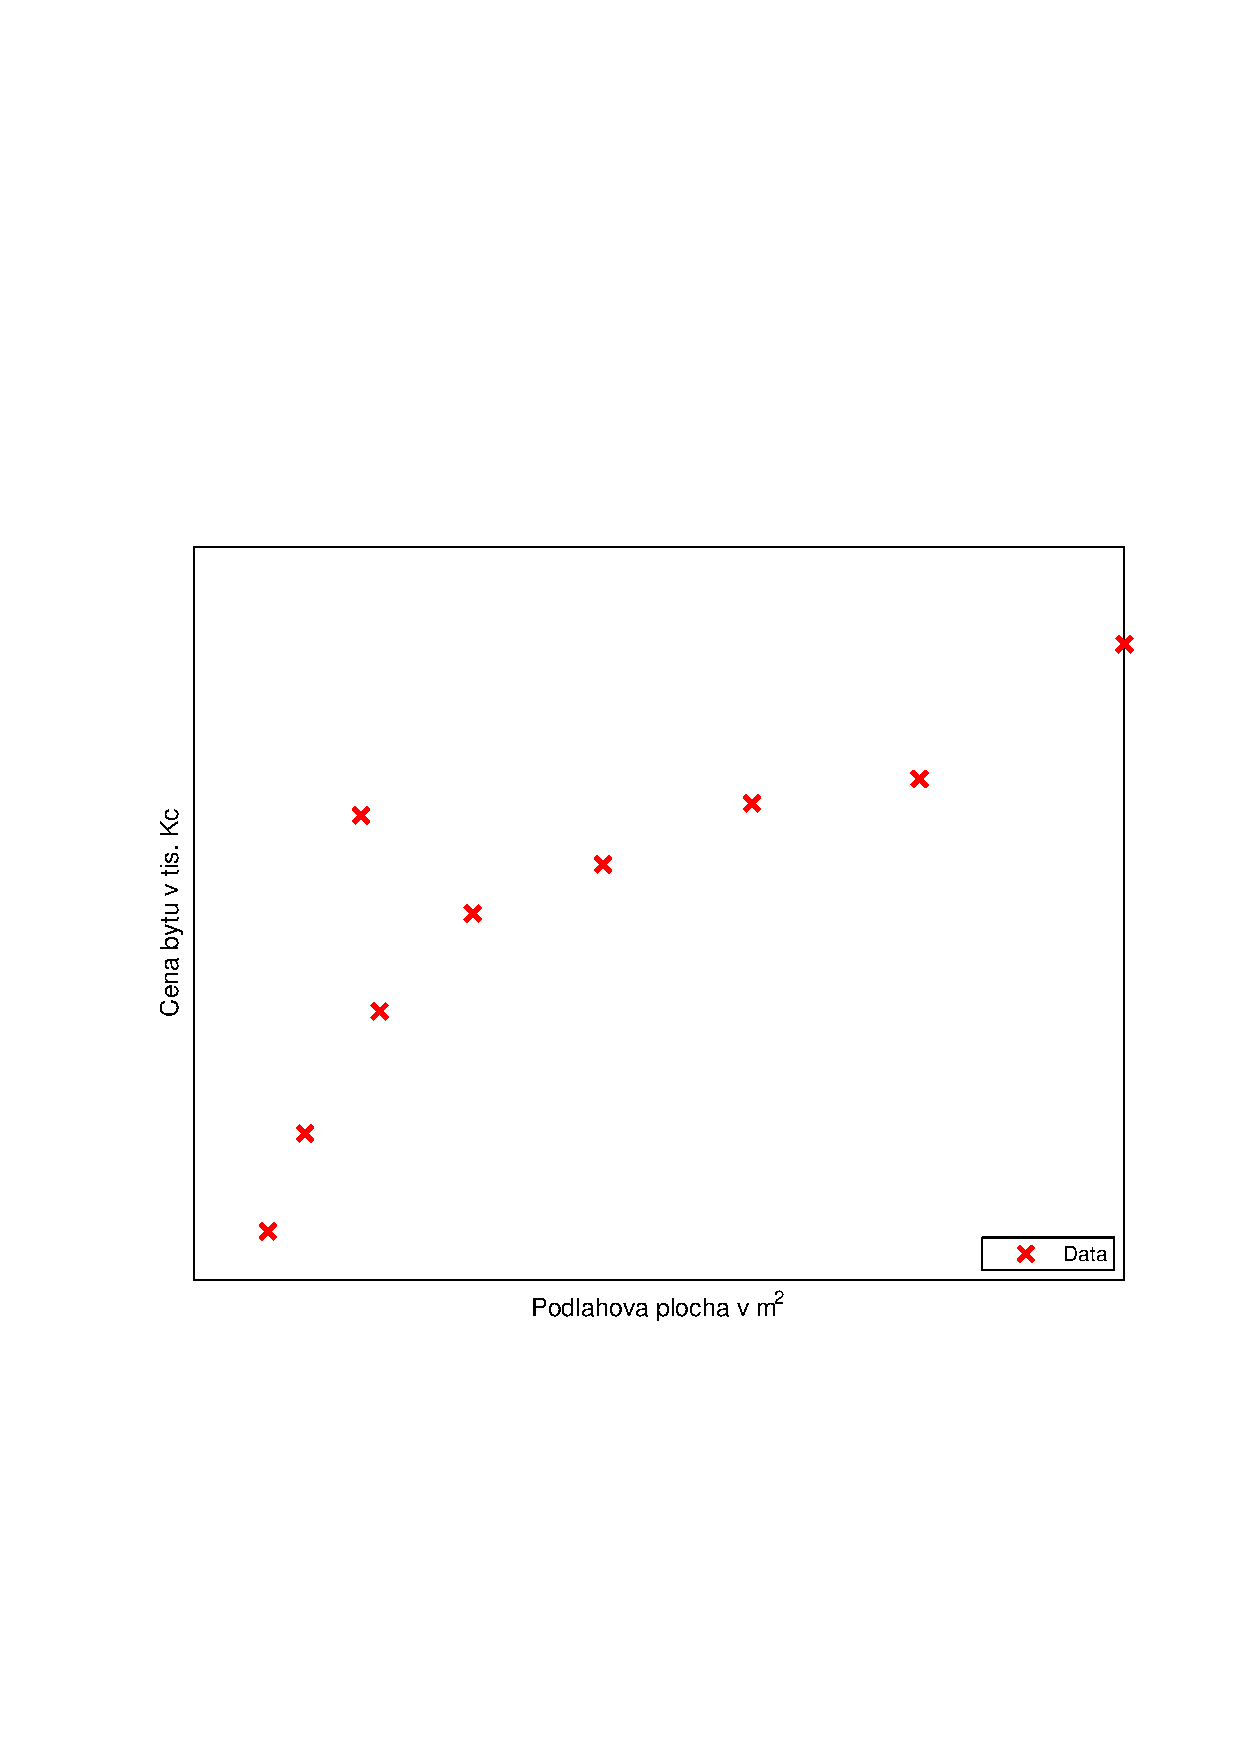
\includegraphics[width = \textwidth, trim = 2.5cm 7cm 2cm 9cm]{./Img/Regularizace/Pretrenovani1D/regrese_0.pdf}
  		\caption{Trénovací data.}
		\label{fig:regrese_0}
	\end{minipage}%
	\hfill
	\begin{minipage}[t]{0.48\textwidth}
		%trim option's parameter order: left bottom right top
		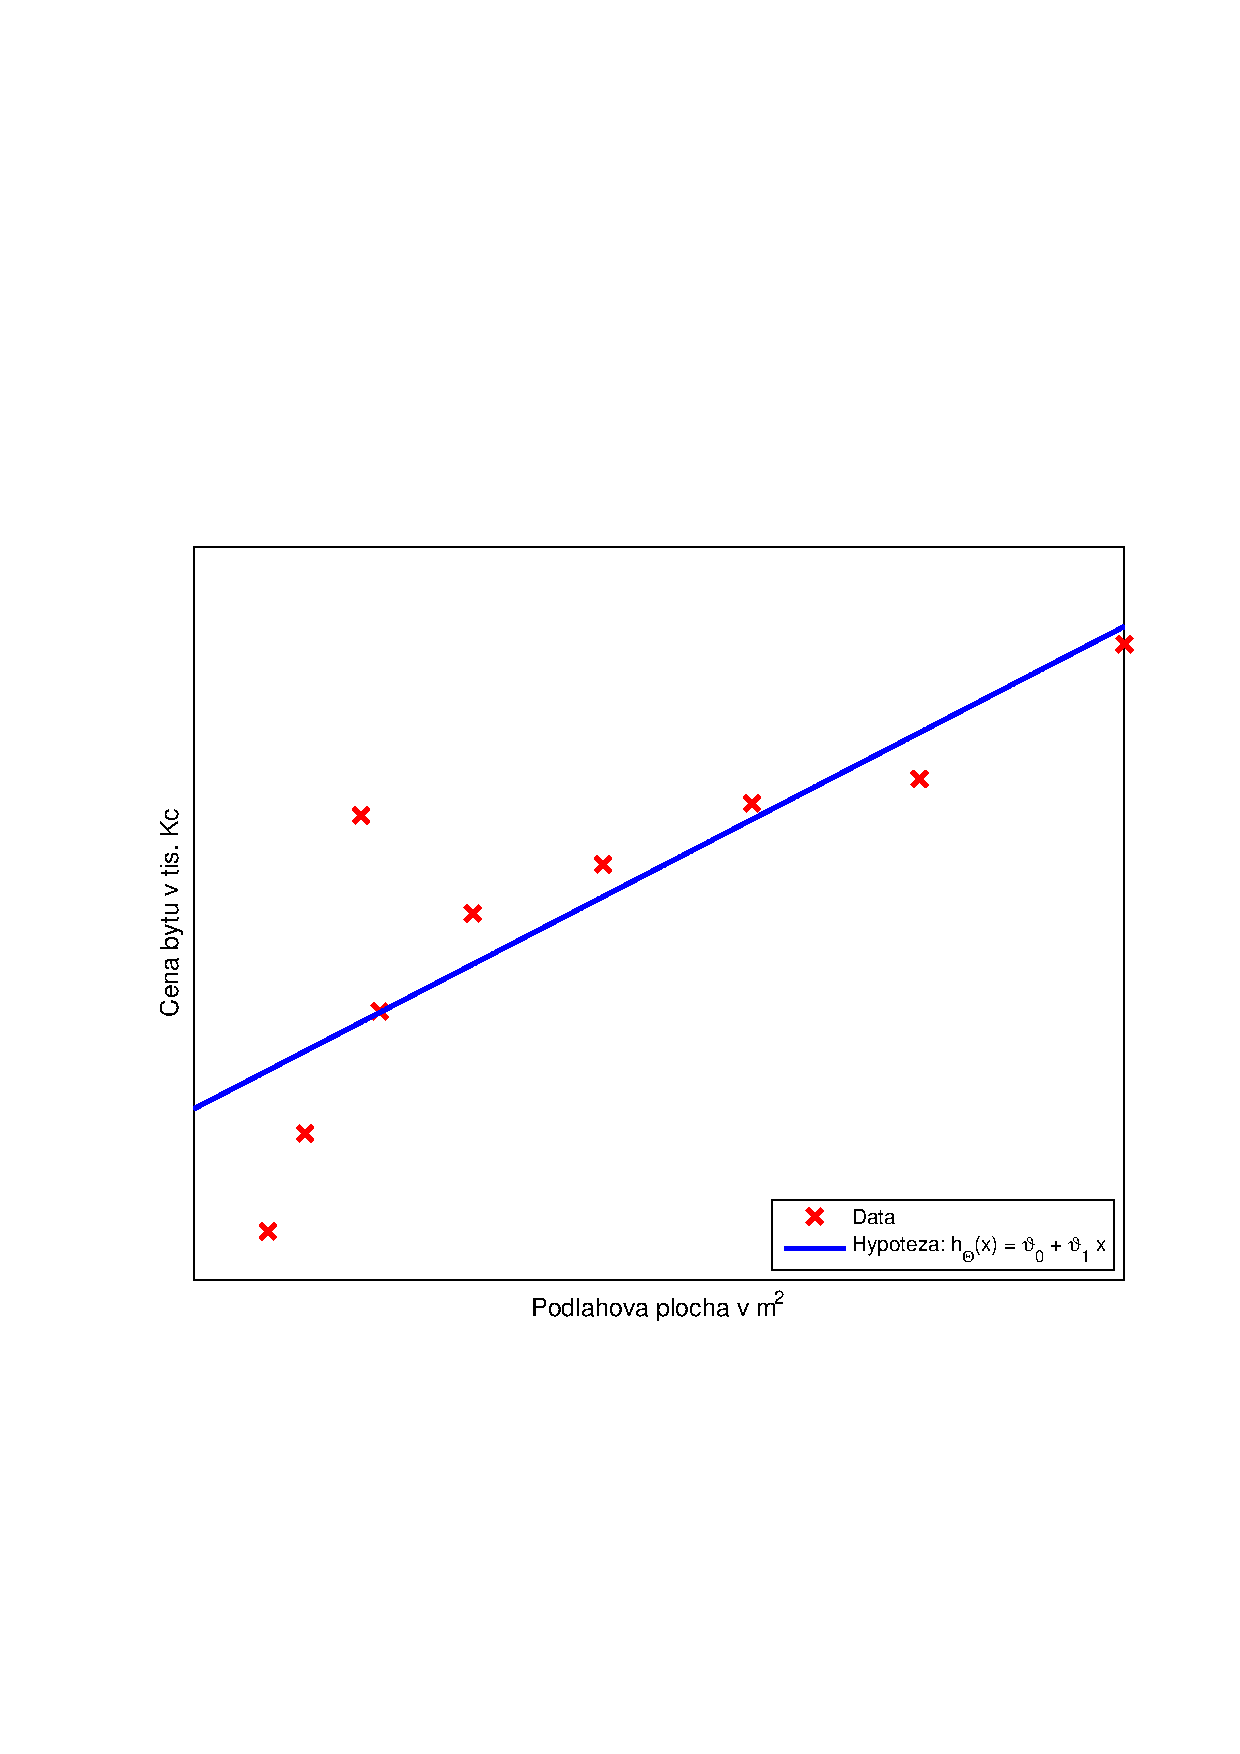
\includegraphics[width = \textwidth, trim = 2.5cm 7cm 2cm 9cm]{./Img/Regularizace/Pretrenovani1D/regrese_1.pdf}
  		\caption{Lineární regrese (\textit{underfit}, \textit{high bias}).}	
		\label{fig:regrese_1}
	\end{minipage}%
\end{figure}
\pagebreak

\par{Na Obr. \ref{fig:regrese_2} lze vidět regresi s hypotézou ve tvaru $h_{\bm{\Theta}} \left( \bm{x} \right) = \vartheta_0 + \vartheta_1 x + \vartheta_2 x^2$, která velmi dobře zobecňuje trénovací data a proto by byla v tomto případě nejlepší volbou.}

\par{Dále na Obr. \ref{fig:regrese_4} lze vidět regresi s hypotézou $h_{\bm{\Theta}} \left( \bm{x} \right) = \vartheta_0 + \vartheta_1 x + \vartheta_2 x^2 + \vartheta_2 x^3 + \vartheta_2 x^4$, jejíž chování je velmi \uv{divoké} a nezobecňuje trénovací data. V tomto případě se snaží hypotéza co nejvíce respektovat trénovací data za cenu ztráty obecnosti. Tento problém se nazývá přetrénování, anglicky \textit{overfitting} nebo \textit{high variance}.}

\begin{figure}[!ht]
	\centering
	\begin{minipage}[t]{0.48\textwidth}
  		%trim option's parameter order: left bottom right top
		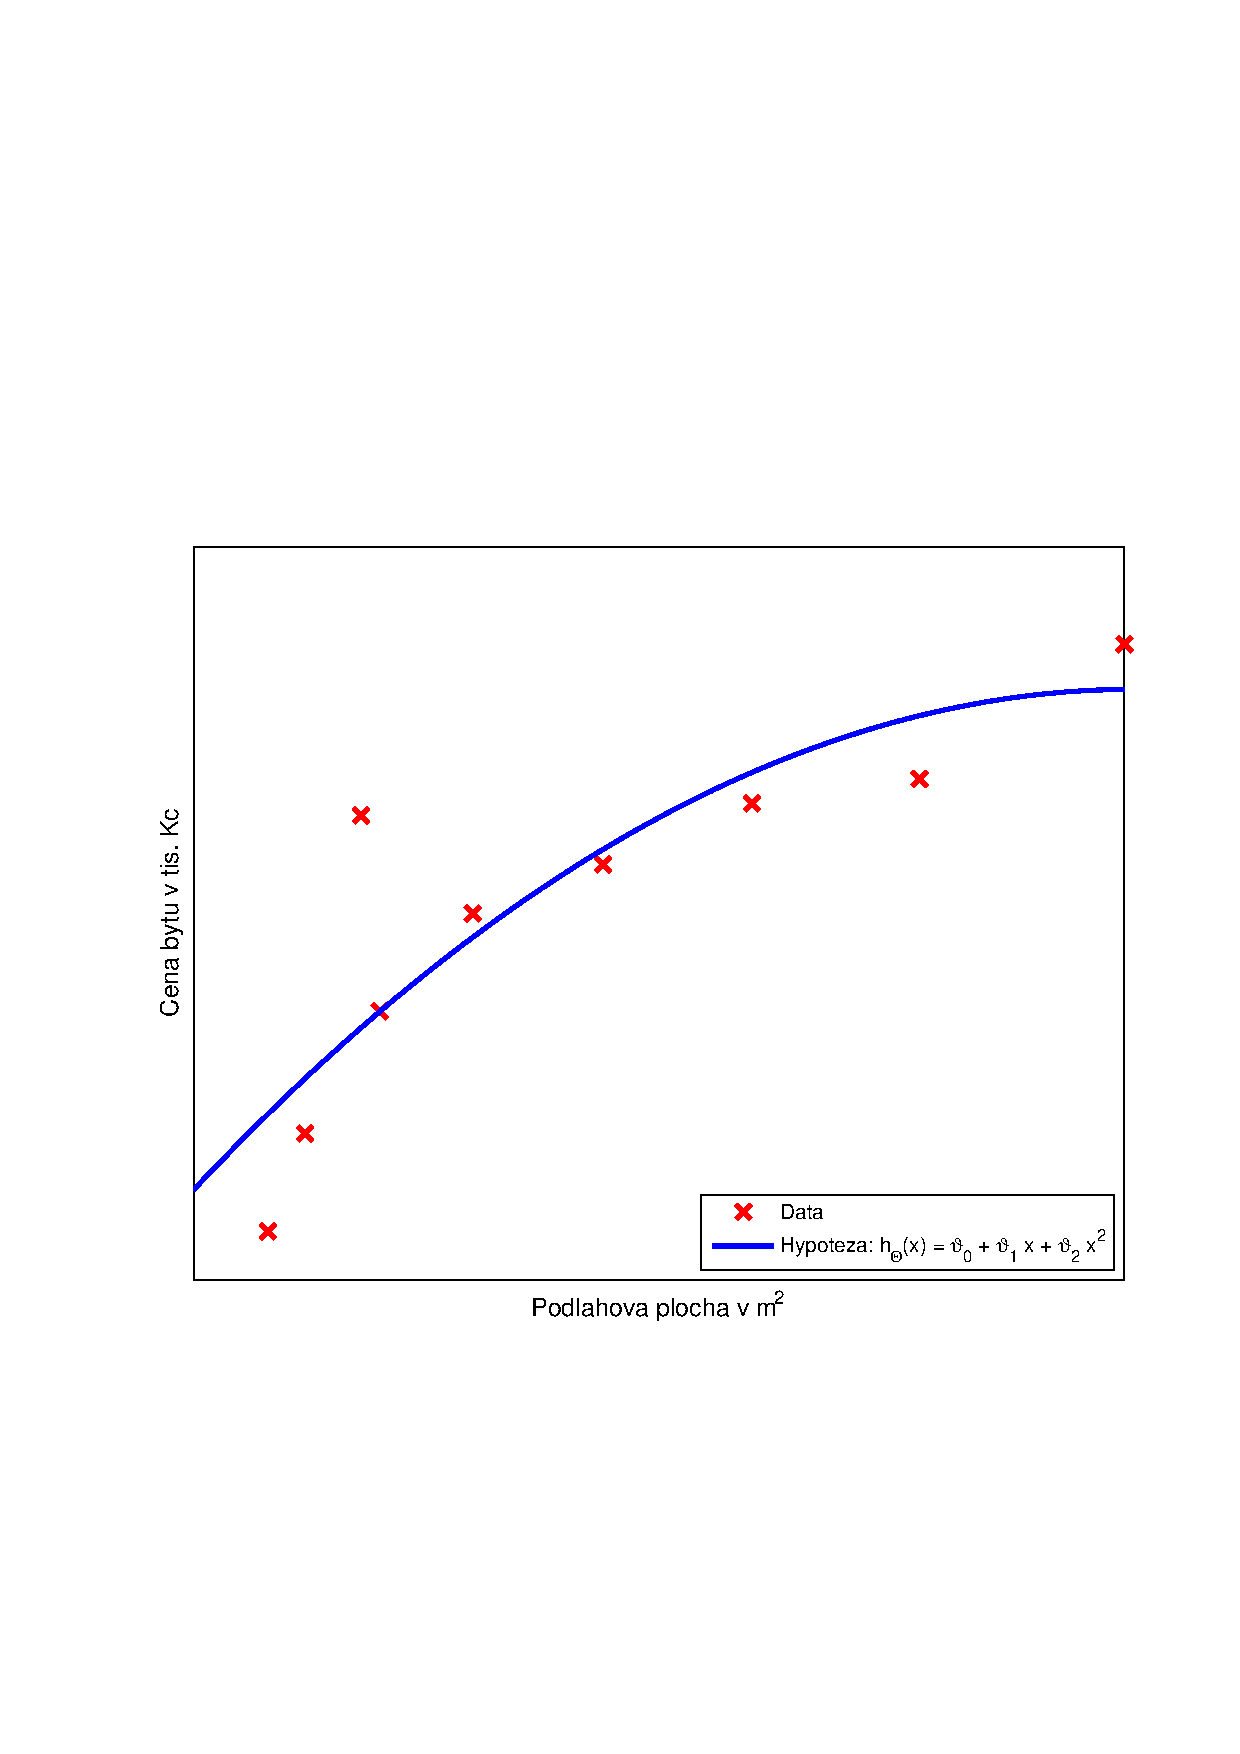
\includegraphics[width = \textwidth, trim = 2.5cm 7cm 2cm 9cm]{./Img/Regularizace/Pretrenovani1D/regrese_2.pdf}
  		\caption{Regrese pomocí hypotézy ve tvaru polynomu druhého stupně (\textit{just right}).}
		\label{fig:regrese_2}
	\end{minipage}%
	\hfill
	\begin{minipage}[t]{0.48\textwidth}
		%trim option's parameter order: left bottom right top
		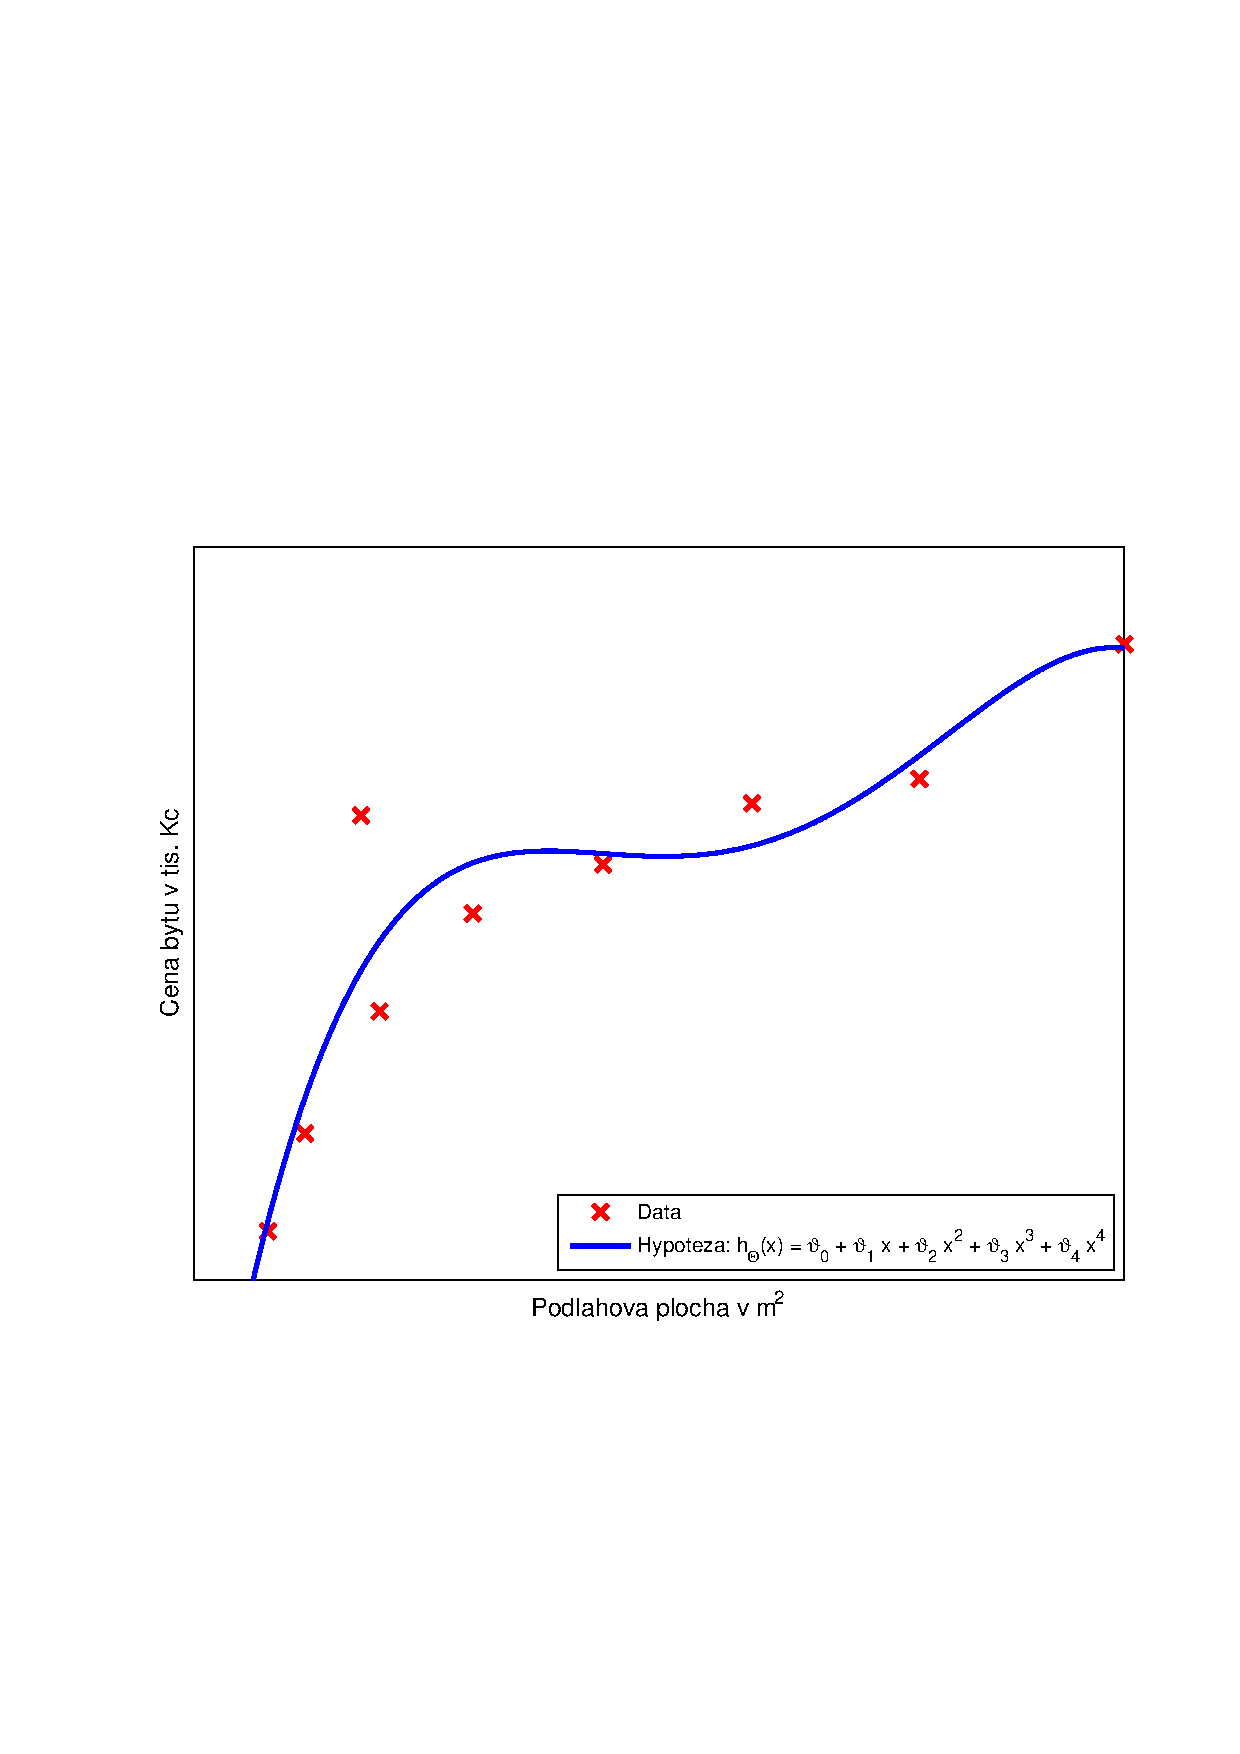
\includegraphics[width = \textwidth, trim = 2.5cm 7cm 2cm 9cm]{./Img/Regularizace/Pretrenovani1D/regrese_4.pdf}
  		\caption{Regrese pomocí hypotézy ve tvaru polynomu čtvrtého stupně (\textit{overfitting}, \textit{high variance}).}
		\label{fig:regrese_4}
	\end{minipage}%
\end{figure}

\subsubsection*{Přetrénování (\textit{overfitting}):}
\par{V případě, že máme příliš mnoho příznaků, hypotéza může velmi dobře respektovat trénovací data $\left( J \left( \bm{\Theta} \right) = \frac{1}{2m} \sum_{i=1}^{m} \left( h_{\bm{\Theta}} \left( \bm{x}^{\left( i \right)} \right) - y^{\left( i \right)} \right)^2 \approx 0 \right)$, ale nebude schopna správně klasifikovat nově příchozí vzorky. Nebude schopna generalizovat, tedy predikce na nově příchozích vzorcích selže.}

\subsubsection*{Možnosti odstranění přetrénování:}
\begin{enumerate}
	\item Redukovat počet příznaků.
		\begin{itemize}
			\item Manuálně zvolit příznaky, které budou zachovány.
			\item Automatická redukce příznaků například PCA.
		\end{itemize}
	\item Regularizace.
		\begin{itemize}
			\item Zachovat všechny příznaky, ale redukovat velikost / váhu parametrů $\vartheta_j$.
			\item Funguje správně pokud máme velké množství příznaků, kde každý malou měrou přispívá k predikci $y$.
		\end{itemize}				
\end{enumerate}



\newpage

















%----ZTRATOVA-FUNKCE-------------------------------------------------------------------------
\subsection{Ztrátová funkce}
\par{V sekci \ref{sec:RegularizaceProblemPretrenovani} jsme si ukázali jak lze pomocí kvadratické hypotézy $h_{\bm{\Theta}} \left( \bm{x} \right) = \vartheta_0 + \vartheta_1 x + \vartheta_2 x^2$ dobře zobecnit naše trénovací data. Dále již víme, že hypotéza ve tvaru $h_{\bm{\Theta}} \left( \bm{x} \right) = \vartheta_0 + \vartheta_1 x + \vartheta_2 x^2 + \vartheta_2 x^3 + \vartheta_2 x^4$ nezobecňuje naší trénovací množinu dat dobře.}
\begin{figure}[!ht]
	\centering
	\begin{minipage}[t]{0.48\textwidth}
  		%trim option's parameter order: left bottom right top
		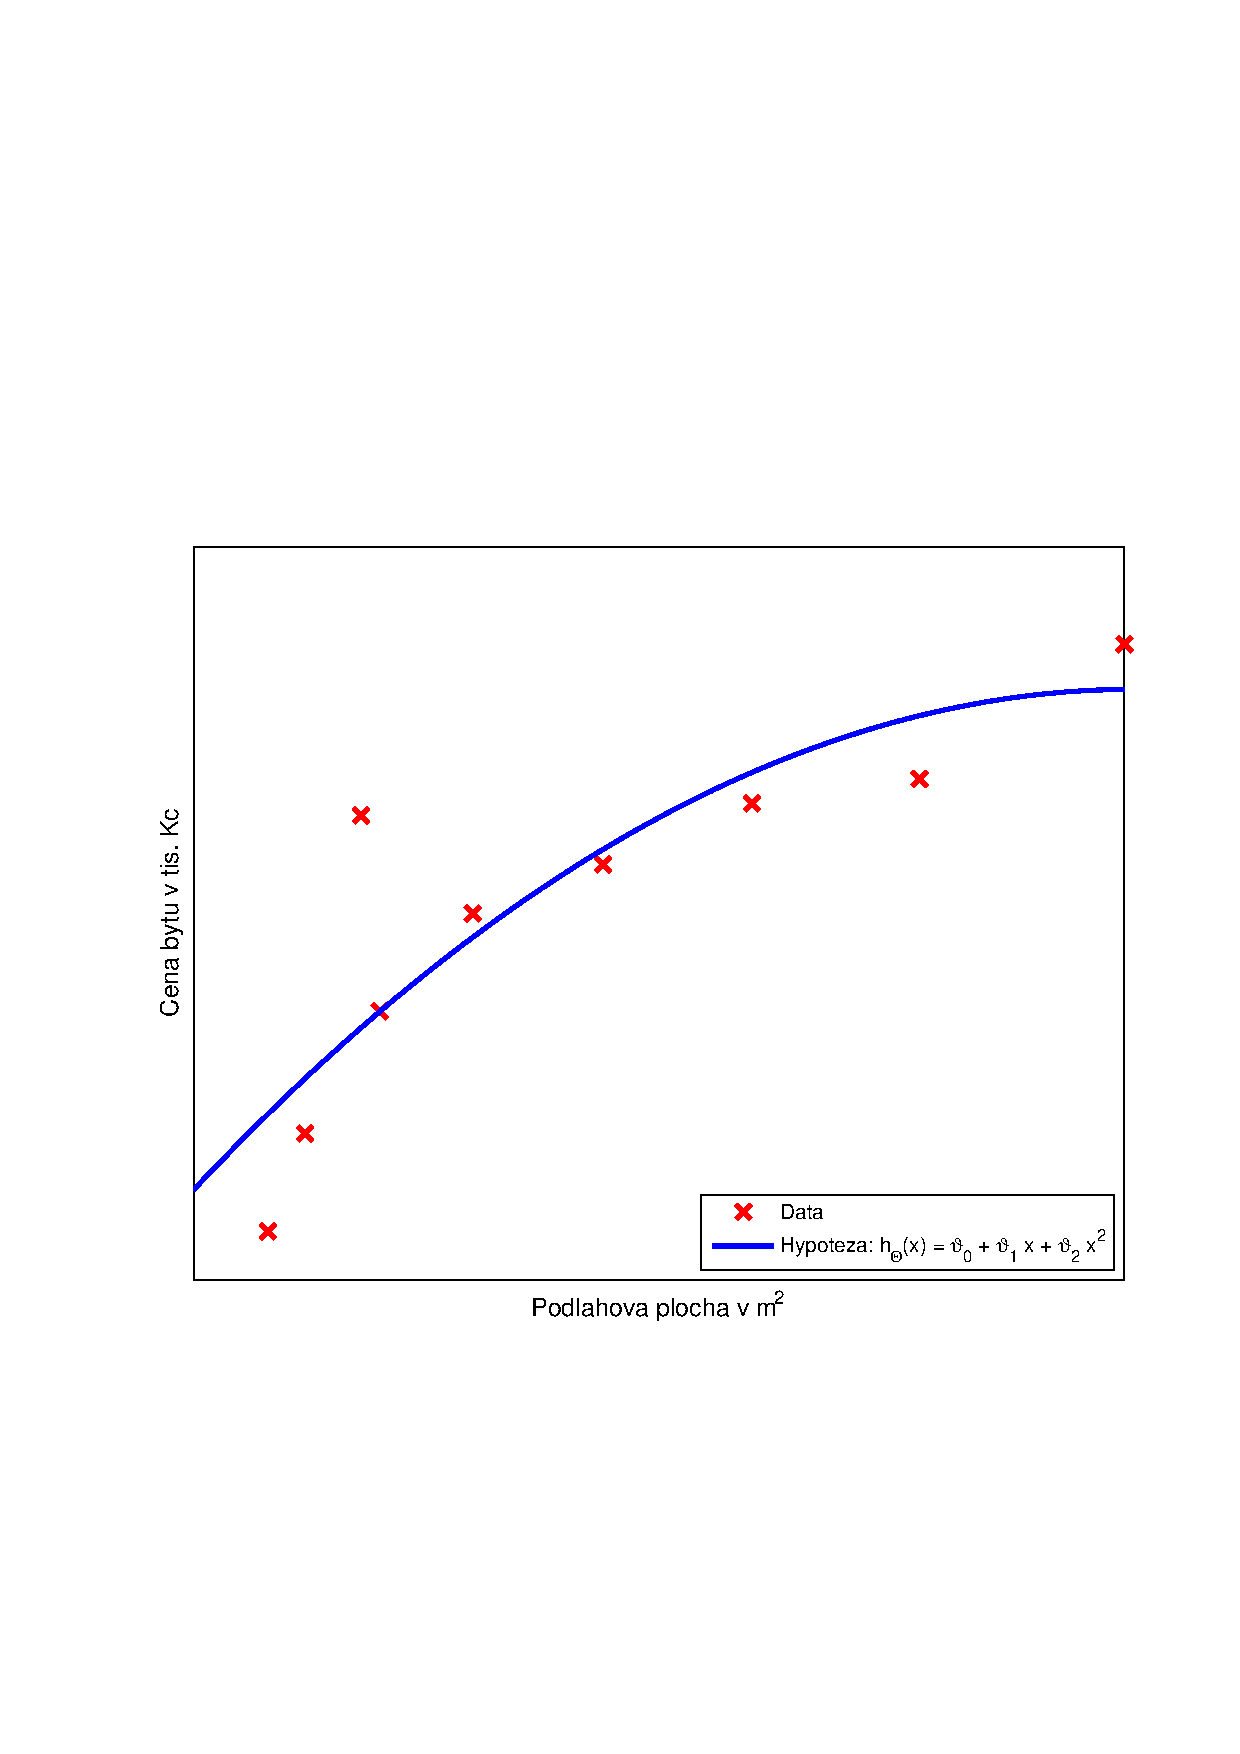
\includegraphics[width = \textwidth, trim = 2.5cm 7cm 2cm 9cm]{./Img/Regularizace/Pretrenovani1D/regrese_2.pdf}
  		\caption{Regrese pomocí hypotézy ve tvaru polynomu druhého stupně (\textit{just right}).}
	\end{minipage}%
	\hfill
	\begin{minipage}[t]{0.48\textwidth}
		%trim option's parameter order: left bottom right top
		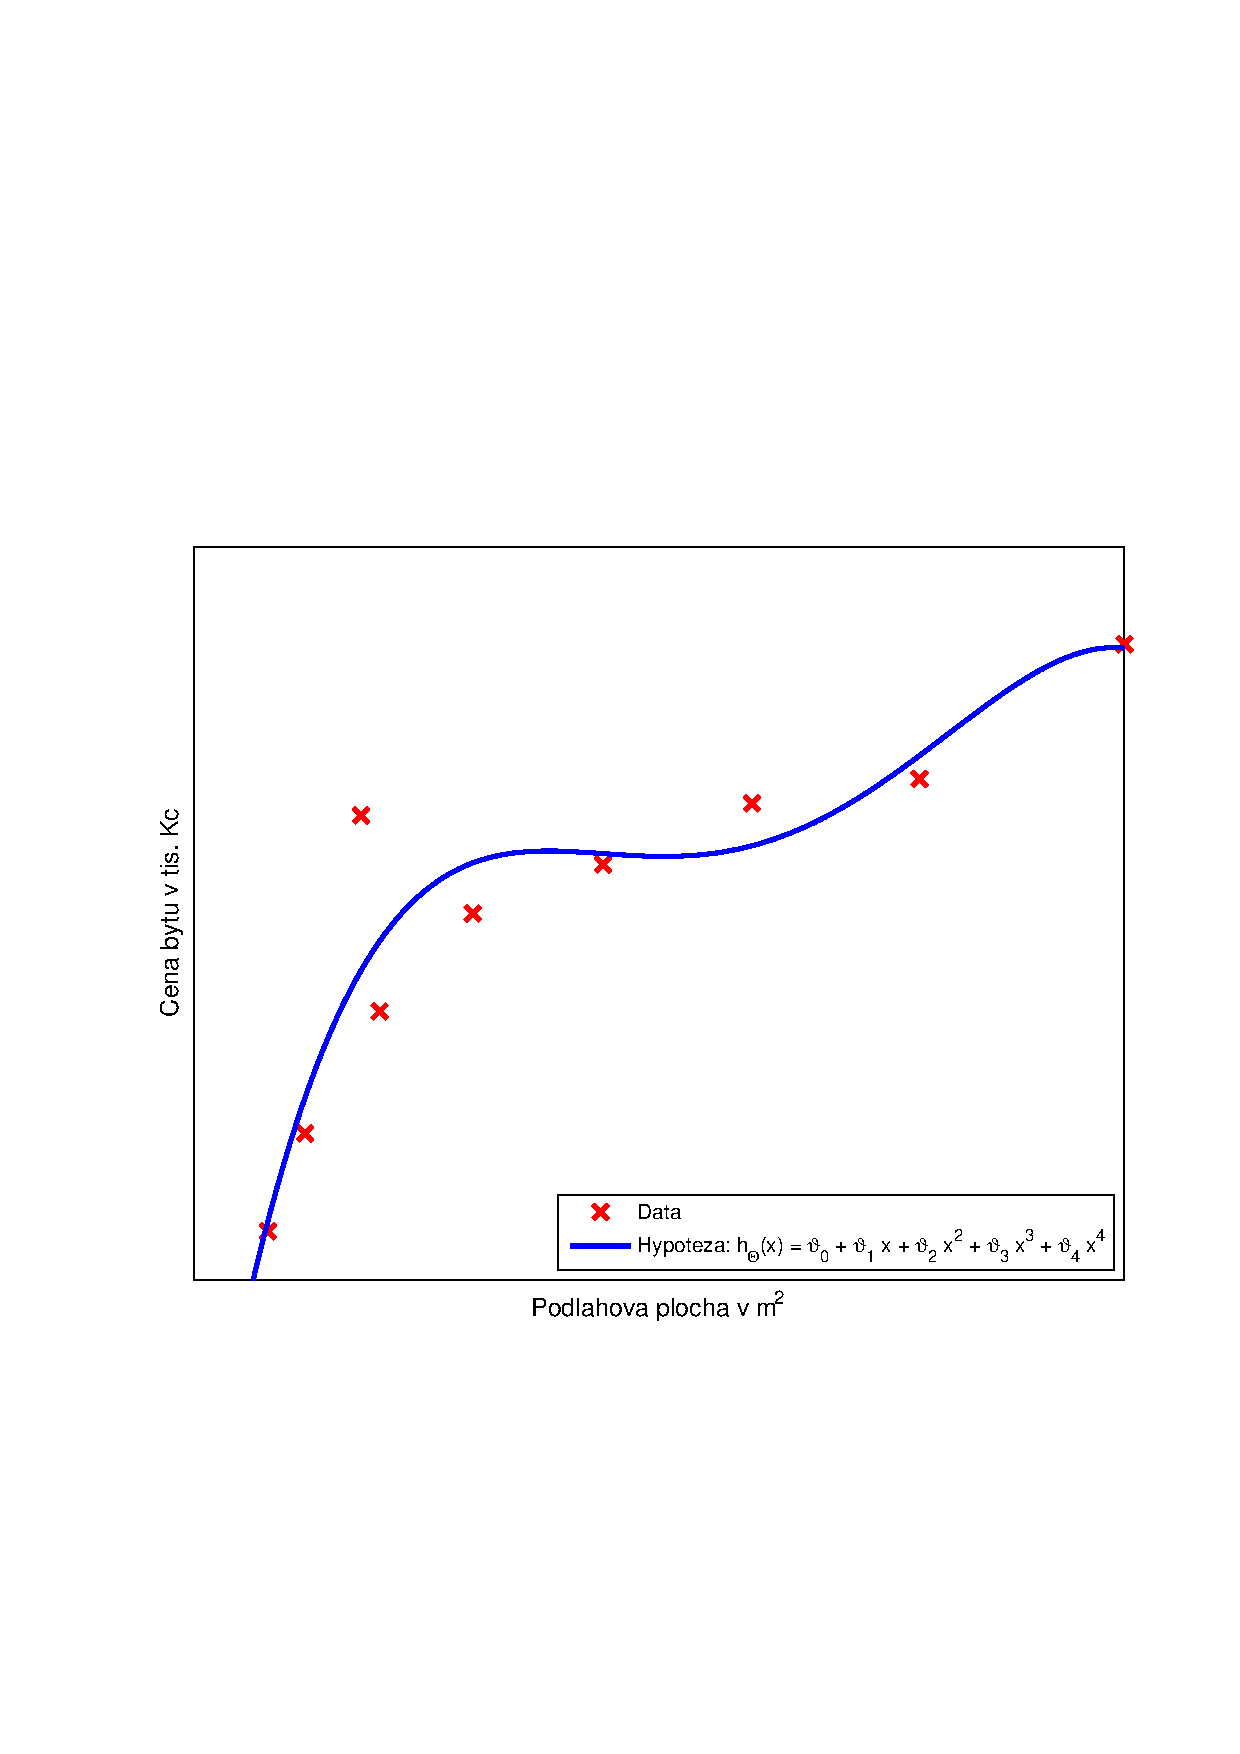
\includegraphics[width = \textwidth, trim = 2.5cm 7cm 2cm 9cm]{./Img/Regularizace/Pretrenovani1D/regrese_4.pdf}
  		\caption{Regrese pomocí hypotézy ve tvaru polynomu čtvrtého stupně (\textit{overfitting}, \textit{high variance}).}
	\end{minipage}%
\end{figure}

\par{Předpokládejme, že budeme penalizovat parametry $\vartheta_3$ a $\vartheta_4$ (jejich hodnoty budou malé). V rovnici \ref{eq:minZtratovaFunkce} je ukázána naše známá optimalizace
\begin{equation}
	\min_{\bm{\Theta}} \frac{1}{2m} \sum_{i=1}^{m} \left( h_{\bm{\Theta}} \left( \bm{x}^{\left( i \right)} \right) - y^{\left( i \right)} \right)^2,
	\label{eq:minZtratovaFunkce}
\end{equation}
kterou můžeme upravit na tvar
\begin{equation}
	\min_{\bm{\Theta}} \frac{1}{2m} \sum_{i=1}^{m} \left( h_{\bm{\Theta}} \left( \bm{x}^{\left( i \right)} \right) - y^{\left( i \right)} \right)^2 + 1000 \vartheta_3^2 + 1000 \vartheta_4^2,
	\label{eq:minZtratovaFunkce1000}
\end{equation}
kde hodnoty 1000 jsou pouze ilustrativní a~reprezentují velká čísla (velké váhy). Tedy pokud bychom chtěli minimalizovat rovnici \ref{eq:minZtratovaFunkce1000}, tak to lze za předpokladu, že $\vartheta_3$ a~$\vartheta_4$ budou malá čísla. V případě, že $\vartheta_3 \approx 0$ a $\vartheta_4 \approx 0$, tak získáme opět náš minimalizační problém jako v~rovnici \ref{eq:minZtratovaFunkce}. Ještě větší dopad to má na tvar hypotézy $h_{\bm{\Theta}} \left( \bm{x} \right) = \vartheta_0 + \vartheta_1 x + \vartheta_2 x^2 + \vartheta_2 x^3 + \vartheta_2 x^4$, která dříve vedla k přetrénování. Ta v~případě, že  $\vartheta_3 \approx 0$ a $\vartheta_4 \approx 0$ přejde na tvar $h_{\bm{\Theta}} \left( \bm{x} \right) = \vartheta_0 + \vartheta_1 x + \vartheta_2 x^2$. Tímto se zbavíme problému přetrénování a~získáme tvar hypotézy, který dobře zobecňuje trénovací data.}

\subsubsection*{Regularizace}
\par{Čím jsou menší hodnoty parametrů $\vartheta_0,\vartheta_1, \ldots , \vartheta_n$, tím \uv{jednodušší} tvar hypotézy získáme a tím méně je tvar hypotézy náchylný k přetrénování. Zapsáno rovnicí
\begin{equation}
	J \left( \bm{\Theta} \right) = \frac{1}{2m} \left( \sum_{i = 1}^{m} \left( h_{\bm{\Theta}} \left( \bm{x}^{\left( i \right)} \right) - y^{\left( i \right)} \right)^2 + \lambda \sum_{j = 1}^{n} \vartheta_j^2 \right),
\end{equation}
kde je nejdříve podotknout, že nová suma s indexem $j$ má jinou mez $n$ než první suma. To je způsobeno tím, že se regularizace vztahuje pouze na parametry $\vartheta_1, \vartheta_2, \ldots , \vartheta_m$, tedy parametr $\vartheta_0$ není regularizován, protože je vždy násoben jedničkou, nepřijde do kontaktu s~příznaky vzorků. Dále parametr $\lambda$ je takzvaný regularizační parametr, který kontroluje vyvážení mezi tím, jak hodně bude regularizace ovlivňovat původní ztrátovou funkci $J \left( \bm{\Theta} \right)$. Regularizace je dána vztahem 
\begin{equation}
	\lambda \sum_{j = 1}^{n} \vartheta_j^2.
\end{equation}
Našim cílem je jako dříve minimalizovat ztrátovou funkci
\begin{equation}
	\min_{\bm{\Theta}} J \left( \bm{\Theta} \right)
\end{equation}}

\par{Co se stane, pokud bude regularizační parametr $\lambda$ příliš velký? Řekněme, že $\lambda = 10^{10}$. Poté hypotéza ve tvaru $h_{\bm{\Theta}} \left( \bm{x} \right) = \vartheta_0 + \vartheta_1 x + \vartheta_2 x^2 + \vartheta_2 x^3 + \vartheta_2 x^4$ přejde na tvar $h_{\bm{\Theta}} \left( \bm{x} \right) = \vartheta_0$ a~výsledný průběh lze vidět na Obr.~\ref{fig:regularizaceUnderfit}}
\begin{figure}[!ht]
	\centering
	%trim option's parameter order: left bottom right top
	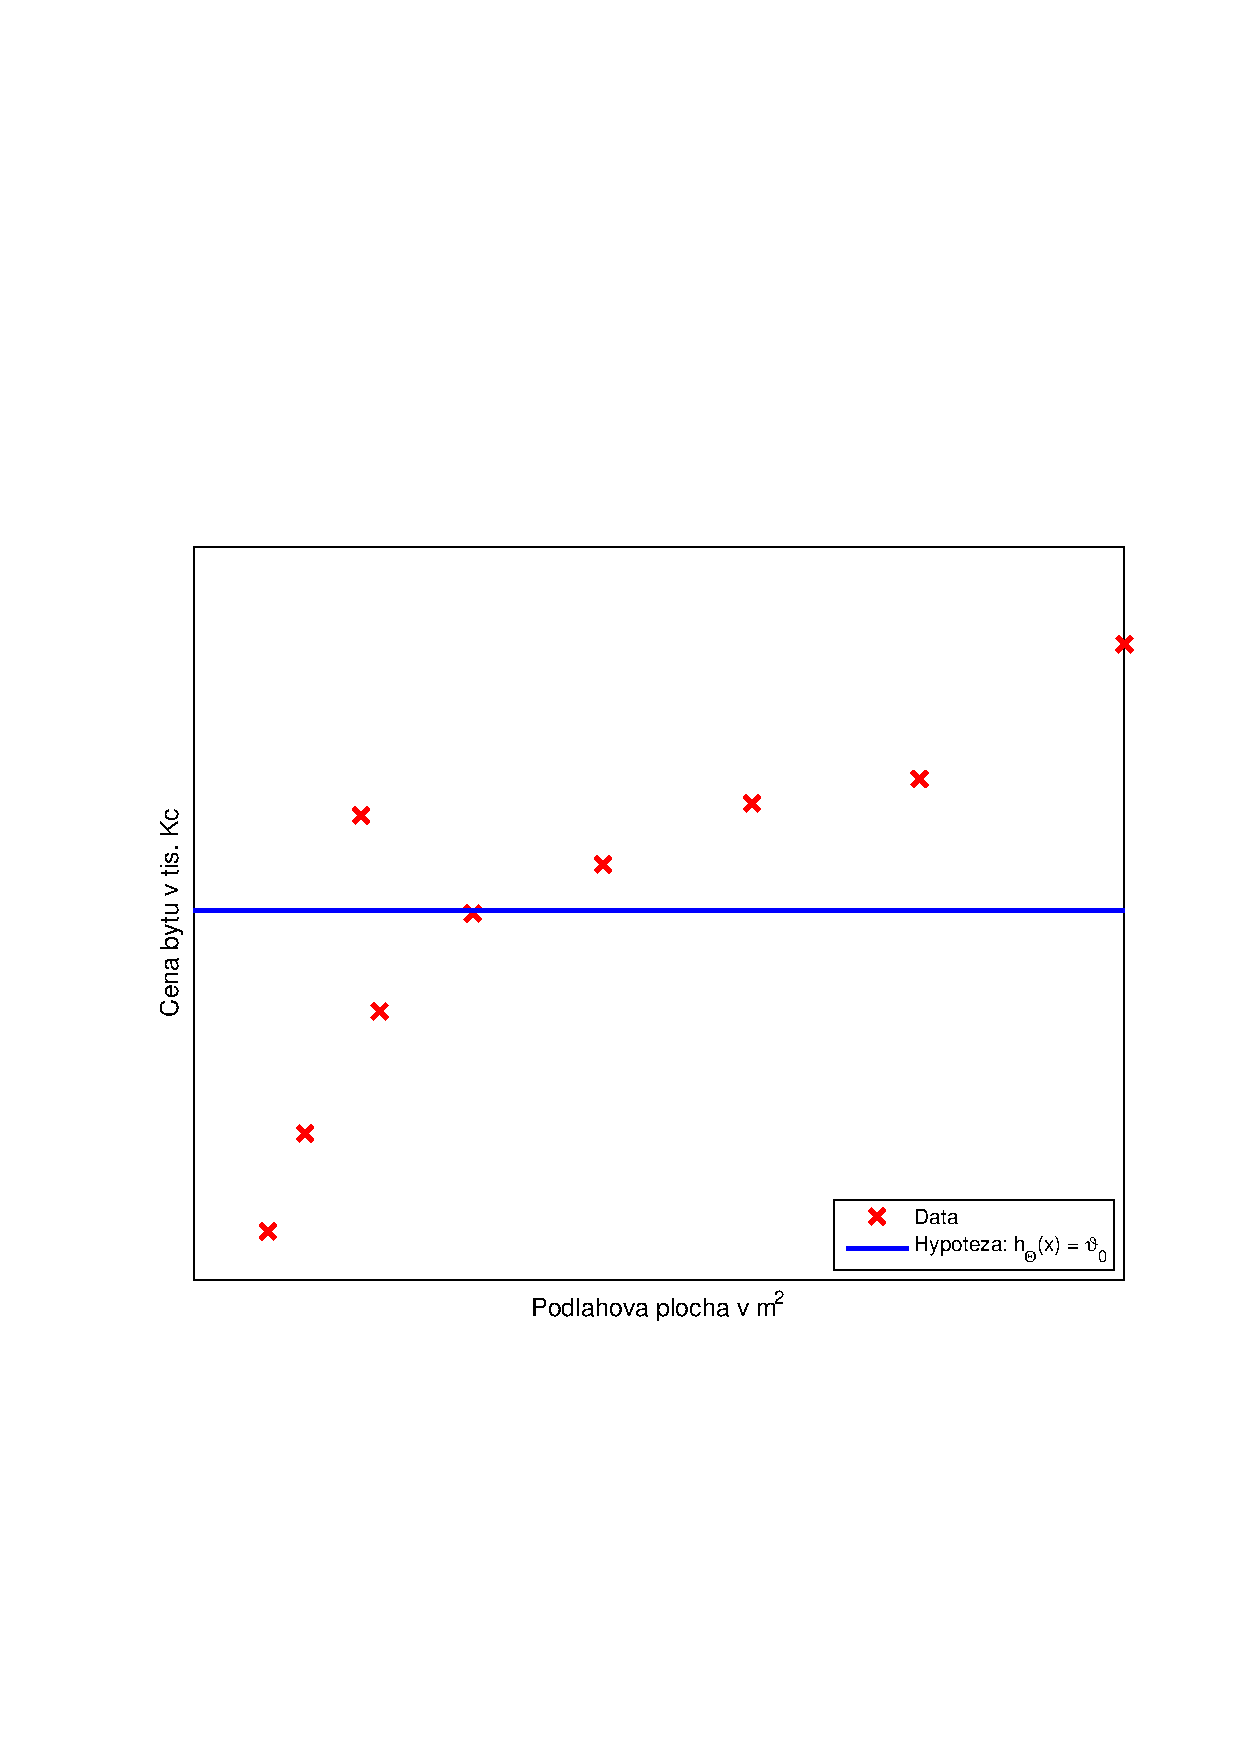
\includegraphics[width = 0.48\textwidth, trim = 2.5cm 7cm 2cm 9cm]{./Img/Regularizace/ZtratovaFunkce/regrese_underfit.pdf}
	\caption{Použití regularizace k získání \textit{underfit} hypotézy.}
	\label{fig:regularizaceUnderfit}
\end{figure}

\par{Z~uvedeného vyplývá, že je nutné volit regularizační parametr~$\lambda$ velmi opatrně. S~velkým~$\lambda$ dosáhneme \textit{underfit} problému a~s~malým~$\lambda$ neodstraníme \textit{overfit} problém.}

\newpage

















%----REGULARIZACE-LINEARNI-REGRESE--------------------------------------------------------------
\subsection{Regularizace lineární regrese}
\label{sec:RegularizaceLinearniRegrese}

\par{Pro lineární regresi máme odvozen gradientní algoritmus a analytické řešení. V této sekci oba algoritmy zobecníme s využitím regularizace.}


\subsubsection*{Regularizace gradientního algoritmu lineární regrese}
\par{Máme naší optimalizační úlohu lineární regrese společně s regularizací
\begin{equation}
	J \left( \bm{\Theta} \right) = \frac{1}{2m} \left( \sum_{i = 1}^{m} \left( h_{\bm{\Theta}} \left( \bm{x}^{\left( i \right)} \right) - y^{\left( i \right)} \right)^2 + \lambda \sum_{j = 1}^{n} \vartheta_j^2 \right),
\end{equation}
snažíme se minimalizovat ztrátovou funkci 
\begin{equation}
	\min_{\bm{\Theta}} J \left( \bm{\Theta} \right)
\end{equation}}

\par{Připomeňme si dříve představený gradientní algoritmus lineární regrese. Opakuj
\begin{equation}
	\vartheta_j = \vartheta_j - \alpha \frac{1}{m} \sum_{i = 1}^{m} \left( h_{\bm{\Theta}} \left( \bm{x}^{\left( i \right)} \right) - y^{\left( i \right)} \right) x_j^{\left( i \right)}, \quad j = 0,1,\ldots ,n .
\end{equation}
Tento algoritmus je možno rozdělit do dvou kroků. Rozdělit výpočet pro $\vartheta_0$ a $\vartheta_{1,\ldots, n}$. Opakuj
\begin{eqnarray}
	&\vartheta_0 &= \vartheta_0 - \alpha \frac{1}{m} \sum_{i = 1}^{m} \left( h_{\bm{\Theta}} \left( \bm{x}^{\left( i \right)} \right) - y^{\left( i \right)} \right) x_0^{\left( i \right)},\\
	%
	&\vartheta_j &= \vartheta_j - \alpha \frac{1}{m} \sum_{i = 1}^{m} \left( h_{\bm{\Theta}} \left( \bm{x}^{\left( i \right)} \right) - y^{\left( i \right)} \right) x_j^{\left( i \right)}, \quad j = 1,2,\ldots ,n .
\end{eqnarray}
Doposud na algoritmu nebylo nic změněno, pouze byl rozepsán do dvou kroků. Protože víme, že na parametr $\vartheta_0$ se regularizace nevztahuje, proto můžeme algoritmus pozměnit a přidat regularizační člen. Následně bude mít gradientní algoritmus tvar. Opakuj
\begin{eqnarray}
	&\vartheta_0 &= \vartheta_0 - \alpha \frac{1}{m} \sum_{i = 1}^{m} \left( h_{\bm{\Theta}} \left( \bm{x}^{\left( i \right)} \right) - y^{\left( i \right)} \right) x_0^{\left( i \right)},\\
		%
	&\vartheta_j &= \vartheta_j - \alpha \left( \frac{1}{m} \sum_{i = 1}^{m} \left( h_{\bm{\Theta}} \left( \bm{x}^{\left( i \right)} \right) - y^{\left( i \right)} \right) x_j^{\left( i \right)} + \frac{\lambda}{m} \vartheta_j \right), \quad j = 1,2,\ldots ,n,	
	\label{eq:LinearniRegreseGradientniAlgProJ1}
\end{eqnarray}
kde platí
\begin{eqnarray}
	\frac{\partial}{\partial \vartheta_0} &J \left( \bm{\Theta} \right)	&= \left( \frac{1}{m} \sum_{i = 1}^{m} \left( h_{\bm{\Theta}} \left( \bm{x}^{\left( i \right)} \right) - y^{\left( i \right)} \right) x_0^{\left( i \right)} \right),\\
	%
	\frac{\partial}{\partial \vartheta_j} &J \left( \bm{\Theta} \right) &= \left( \frac{1}{m} \sum_{i = 1}^{m} \left( h_{\bm{\Theta}} \left( \bm{x}^{\left( i \right)} \right) - y^{\left( i \right)} \right) x_j^{\left( i \right)} + \frac{\lambda}{m} \vartheta_j \right), \quad j = 1,2,\ldots ,n.
\end{eqnarray}}

\par{Rovnice \ref{eq:LinearniRegreseGradientniAlgProJ1} lze přepsat do tvaru 
\begin{equation}
	\vartheta_j = \vartheta_j \left( 1 - \alpha \frac{\lambda}{m} \right) - \alpha \frac{1}{m} \sum_{i = 1}^{m} \left( h_{\bm{\Theta}} \left( \bm{x}^{\left( i \right)} \right) - y^{\left( i \right)} \right) x_j^{\left( i \right)},
\end{equation}
kde platí
\begin{equation}
	1 - \alpha \frac{\lambda}{m} < 1.
\end{equation}}



\subsubsection*{Regularizace analytického řešení lineární regrese}

\par{Připomeňme si}
\begin{equation}
	\bm{X} = \left[ \left( \bm{x}^{\left( 1 \right)} \right)^{\top}, \ldots, \left( \bm{x}^{\left( m \right)} \right)^{\top}  \right]^{\top},\quad  \bm{X} \in  \mathcal{R}^{m \times \left( n + 1 \right)}
\end{equation}
a
\begin{equation}
	\bm{y} = \left[ y^{\left( 1 \right)}, \ldots, y^{\left( m \right)}   \right]^{\top}, \quad \bm{y} \in \mathcal{R}^{m}.
\end{equation}
Analytické řešení pro výpočet $\bm{\Theta}$ má tvar
\begin{equation}
	\bm{\Theta} = \left( \bm{X}^{\top} \bm{X} \right)^{-1} \bm{X}^{\top} y.
\end{equation}
Cílem je minimalizovat ztrátovou funkci
\begin{equation}
	\min_{\bm{\Theta}} J \left( \bm{\Theta} \right).
\end{equation}

\par{Pokud využijeme regularizaci, tak naše analytické řešení přejde na tvar
\begin{equation}
	\bm{\Theta} = \left( \bm{X}^{\top} \bm{X} + \lambda 
	\left[ \begin{array}{ccccc}
		0 & 0 & 0 & 0 & 0\\
		0 & 1 & 0 & 0 & 0 \\
		0 & 0 & 1 & 0 & 0\\
		0 & 0 & 0 & \ddots & \vdots\\
		0 & 0 & 0 & \cdots & 1
	\end{array} \right] \right)^{-1} \bm{X}^{\top} y
\end{equation}
kde nová matice má velikost $\mathcal{R}^{\left( n + 1 \right) \times \left( n+ 1 \right)}$}

\subsubsection*{Rozšíření}
\par{Předpokládejme, že $m \leq n$, kde $m$ je počet vzorků a $n$ je počet příznaků a 
\begin{equation}
	\bm{\Theta} = \left( \bm{X}^{\top} \bm{X} \right)^{-1} \bm{X}^{\top} y,
\end{equation}
pak je matice $\bm{X}^{\top} \bm{X} $ neinvertovatelná / singulární.}

\par{Pro výpočet lze v tomto případě využít pseudoinverze, konkrétně v~MATLABu k~tomuto účelu slouží funkce \textit{pinv()}.}
\lstinputlisting[language = Matlab]{./Img/Regularizace/noninvertibilityXX/XX.m}

\par{Pokud $\lambda > 0$}
\begin{equation}
	\bm{\Theta} = \left( \underbrace{ \bm{X}^{\top} \bm{X} + \lambda 
	\left[ \begin{array}{ccccc}
		0 & ~ & ~ & ~ & ~\\
		~ & 1 & ~ & ~ & ~ \\
		~ & ~ & 1 & ~ & ~\\
		~ & ~ & ~ & \ddots & ~\\
		~ & ~ & ~ & ~ & 1
	\end{array} \right]}_{\text{Matice musí být invertovatelná}}  \right)^{-1} \bm{X}^{\top} y
\end{equation}

\newpage






















%----REGULARIZACE-BINARNI REGRESE--------------------------------------------------------------
\subsection{Regularizace binární regrese}
\par{Pro binární regresi jsme dříve mluvili o dvou typech optimalizace. Mluvili jsme o tom, jak použít gradientní algoritmus a jak použít pokročilé metody optimalizace. V této sekci si ukážeme, jak tyto přístupy upravit, aby využily regularizace.}

\subsubsection*{Regularizace binární regrese}

\par{Dříve jsme si ukázali, že binární regrese je náchylná na přetrénování v případě, kdy zvolíme vysoký stupeň polynomu reprezentující naší hypotézu, například
\begin{equation}
	h_{\bm{\Theta}} \left( \bm{x} \right) = g \left( \vartheta_0  + \vartheta_1 x_1 + \vartheta_2 x^2_1 + \vartheta_3 x_1^2 x_2 + \vartheta_4 x_1^2 x_2^2 + \vartheta_5 x_1^2 x_2^3 + \ldots \right),
	\label{eq:BReg_hypo}
\end{equation}
pro takovouto složitou hypotézu můžeme dostat dělící křivku velmi variabilní a velmi respektující rozdělení trénovacích dat, tedy křivku, která nedostatečně zobecňuje.
\begin{figure}[!ht]
	\centering
	%trim option's parameter order: left bottom right top
	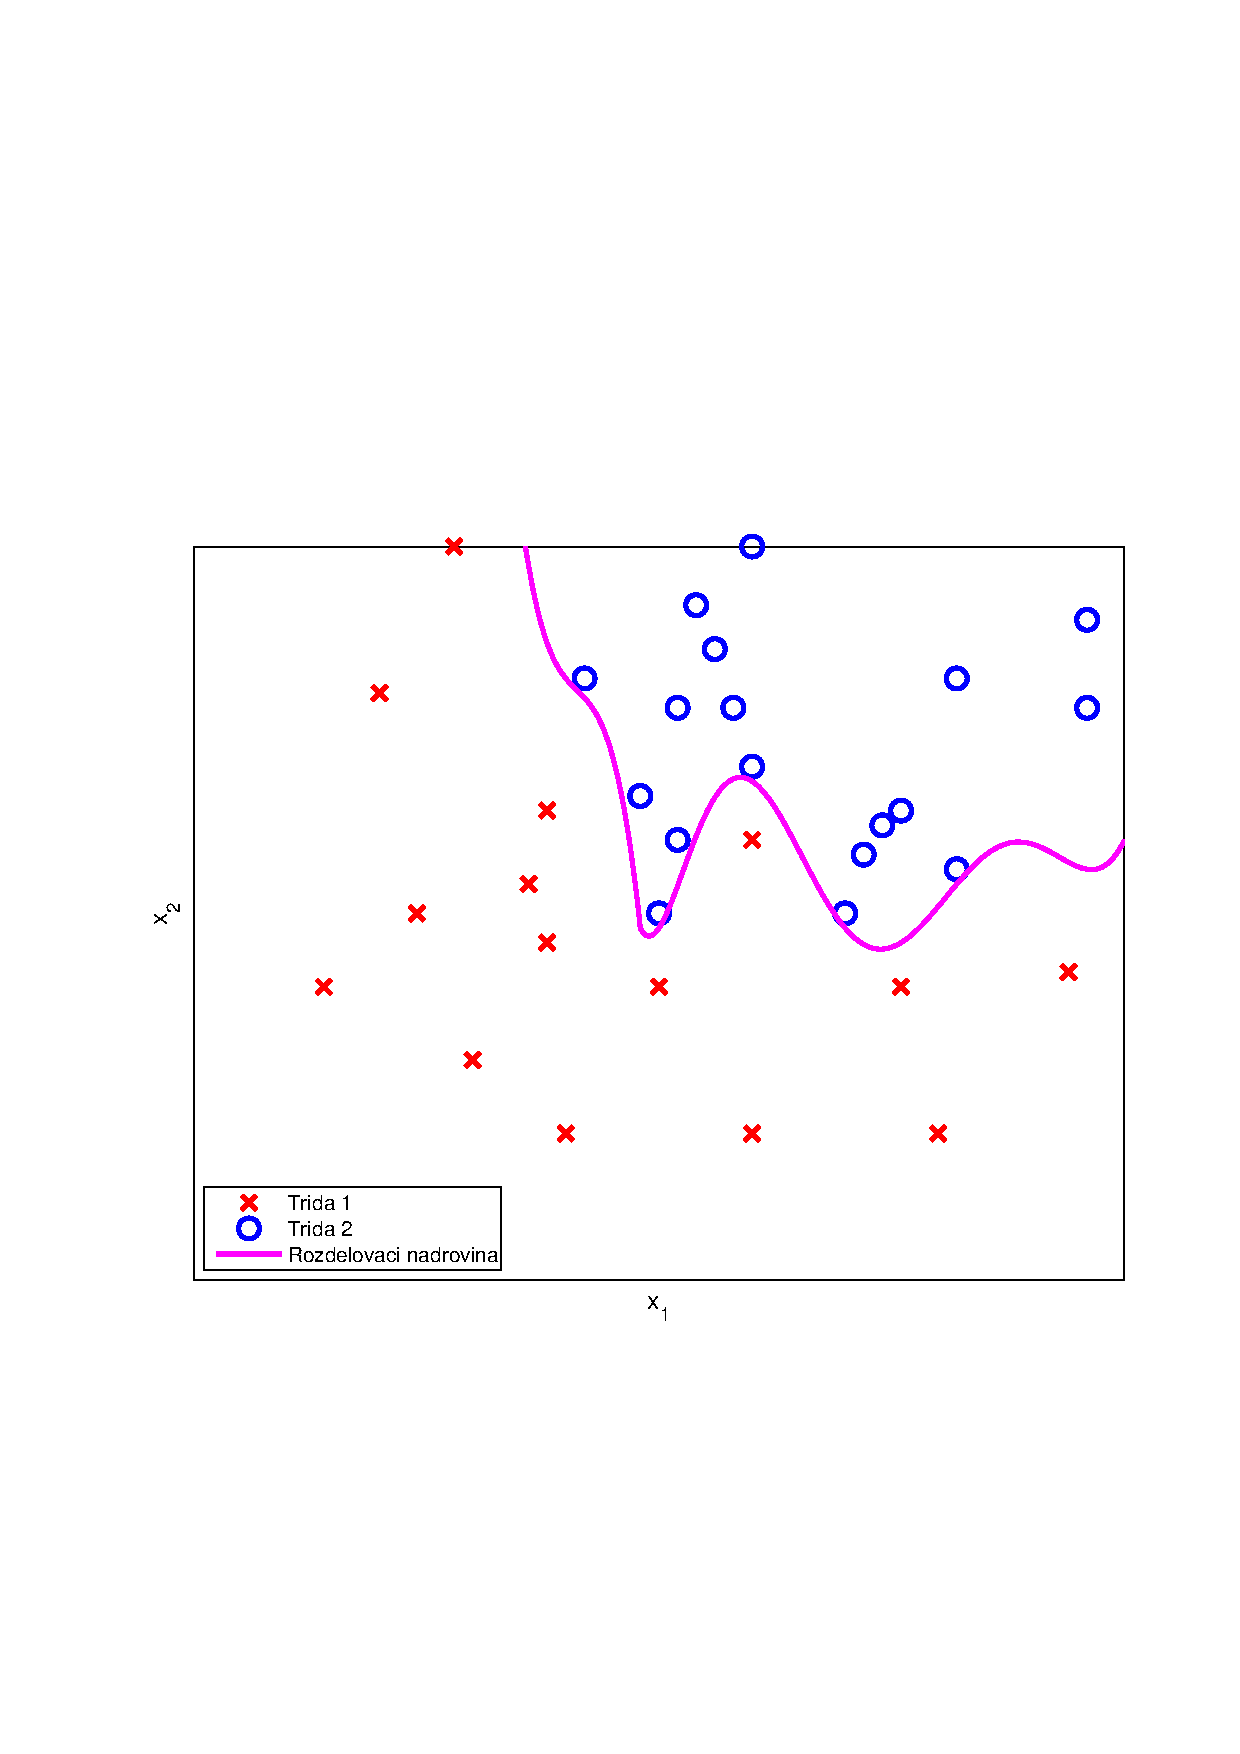
\includegraphics[width = 0.48\textwidth, trim = 2.5cm 7cm 2cm 9cm]{./Img/Regularizace/binarniRegrese/regularizace_binarni_regrese.pdf}
	\caption{Možný výsledek s použitím hypotézy z rovnice \ref{eq:BReg_hypo}.}
	\label{fig:binaryRegularizationExample}
\end{figure}
}

\par{Ztrátová funkce pro binární regresi má tvar
\begin{equation}
	J \left( \bm{\Theta} \right) =  - \left[ \frac{1}{m} \sum_{i = 1}^{m} y^{ \left( i \right)} \log \left( h_{\bm{\Theta}} \left( \bm{x}^{\left( i \right)} \right) \right) + \left( 1 - y^{\left( i \right)} \right) \log \left( 1 - h_{\bm{\Theta}} \left( \bm{x}^{\left( i \right)} \right) \right) \right]
\end{equation}
a její modifikací získáme regularizovaný tvar ztrátové funkce
\begin{equation}
	J \left( \bm{\Theta} \right) =  - \left[ \frac{1}{m} \sum_{i = 1}^{m} y^{ \left( i \right)} \log \left( h_{\bm{\Theta}} \left( \bm{x}^{\left( i \right)} \right) \right) + \left( 1 - y^{\left( i \right)} \right) \log \left( 1 - h_{\bm{\Theta}} \left( \bm{x}^{\left( i \right)} \right) \right) \right] + \frac{\lambda}{2m} \sum_{j = 1}^{n} \vartheta_j^2
\end{equation}
přidaná suma je jen do $n$, jelikož se neregularizuje složka $\vartheta_0$, která je vždy rovna jedné a~není v~součinu se žádnou proměnnou $x$, $y$. Tvar ztrátové funkce společně s~regularizací bude naší rozdělovací nadrovinu více zobecňovat a~pomůže nám řešit problém přetrénování.}

\par{Implementace bude provedena následovně: opakuj
\begin{eqnarray}
	&\vartheta_0 &= \vartheta_0 - \alpha \frac{1}{m} \sum_{i = 1}^{m} \left( h_{\bm{\Theta}} \left( \bm{x}^{\left( i \right)} \right) - y^{\left( i \right)} \right) x_0^{\left( i \right)}\\
	&\vartheta_j &= \vartheta_j - \alpha \left[ \frac{1}{m} \sum_{i = 1}^{m} \left( h_{\bm{\Theta}} \left( \bm{x}^{\left( i \right)} \right) - y^{\left( i \right)} \right) x_j^{\left( i \right)} + \frac{\lambda}{m} \vartheta_j \right], \qquad j = 1, 2, 3, \ldots , n,
	\label{eq:gradDescent_regularizace2rce}
\end{eqnarray}
kde 
\begin{equation}
	h_{\bm{\Theta}} \left( \bm{x} \right) = \frac{1}{1 + e^{- \bm{\Theta}^{\top} \bm{x} }}.
\end{equation}
Z~rovnice \ref{eq:gradDescent_regularizace2rce} lze vidět, že platí
\begin{equation}
	\frac{\partial}{\partial \vartheta_j} J \left( \bm{\Theta} \right) = \frac{1}{m} \sum_{i = 1}^{m} \left( h_{\bm{\Theta}} \left( \bm{x}^{\left( i \right)} \right) - y^{\left( i \right)} \right) x_j^{\left( i \right)} + \frac{\lambda}{m} \vartheta_j.
\end{equation}}





\subsubsection*{Regularizace pokročilé optimalizace}
\par{Nyní bude nastíněno jak využit pokročilé optimalizace v MATLABu. Nechť náš vektor parametrů $\bm{\Theta}$ odpovídá
\begin{equation}
	\bm{\Theta} = \left[ \vartheta_0 , \vartheta_1, \ldots , \vartheta_n \right]^{\top} = \left[ theta(1), theta(2), \ldots, theta(n + 1 ) \right]
\end{equation}
(z důvodu, že MATLAB indexuje od jedničky).
\lstinputlisting[language = Matlab]{./Img/Regularizace/AdvancedOptimalization/costFunction.m}
\begin{equation}
	J \left( \bm{\Theta} \right) = \left[ 
	- \frac{1}{m} \sum_{i = 1}^{m} y^{\left( i \right)} 
	\log \left( h_{\bm{\Theta}} \left( \bm{x}^{\left( i \right) } \right) \right)
	+ \left( 1 - y^{\left( i \right)} \right)
	\log \left( 1 - h_{\bm{\Theta}} \left( \bm{x}^{\left( i \right)} \right) \right) \right] + \frac{\lambda}{2m} \sum_{j = 1}^{n} \vartheta_j^2
\end{equation}
dále výpočet gradientu
\lstinputlisting[language = Matlab]{./Img/Regularizace/AdvancedOptimalization/grad1.m}
\begin{equation}
	\frac{\partial}{\partial \vartheta_0} J \left( \bm{\Theta} \right) = \frac{1}{m} \sum_{i = 1}^{m} \left( h_{\bm{\Theta}} \left( \bm{x}^{\left( i \right)} \right) - y^{\left( i \right)} \right) x_0^{\left( i \right)},
\end{equation}
\lstinputlisting[language = Matlab]{./Img/Regularizace/AdvancedOptimalization/grad2.m}
\begin{equation}
	\frac{\partial}{\partial \vartheta_1} J \left( \bm{\Theta} \right) = \left[ \frac{1}{m} \sum_{i = 1}^{m} \left( h_{\bm{\Theta}} \left( \bm{x}^{\left( i \right)} \right) - y^{\left( i \right)} \right) x_1^{\left( i \right)} \right] + \frac{\lambda}{m} \vartheta_1,
\end{equation}
\lstinputlisting[language = Matlab]{./Img/Regularizace/AdvancedOptimalization/grad3.m}
\begin{equation}
	\frac{\partial}{\partial \vartheta_2} J \left( \bm{\Theta} \right) = \left[ \frac{1}{m} \sum_{i = 1}^{m} \left( h_{\bm{\Theta}} \left( \bm{x}^{\left( i \right)} \right) - y^{\left( i \right)} \right) x_2^{\left( i \right)} \right] + \frac{\lambda}{m} \vartheta_2,
\end{equation}
\lstinputlisting[language = Matlab]{./Img/Regularizace/AdvancedOptimalization/gradN+1.m}
\begin{equation}
	\ldots
\end{equation}}






\newpage











































%----UCENI-S-UCITELEM-----------------------------------------------------------------
\section{Učení s učitelem}
\label{sec:UvodUceniSUcitelem}

\par{\textbf{Učení s učitelem} je metoda strojového učení pro učení funkce z trénovacích dat. Trénovací data sestávají ze dvojic vstupních objektů (typicky vektorů příznaků) a požadovaného výstupu. Výstup funkce může být spojitá hodnota (při regresi) anebo může předpovídat označení třídy vstupního objektu (při klasifikaci). Úloha algoritmu učení je předpovídat výstupní hodnotu funkce pro každý platný vstupní objekt poté, co zpracuje trénovací příklady (tj. dvojice vstup a požadovaný výstup). Aby to dokázal, musí algoritmus zobecnit prezentovaná data na nové situace (vstupy) \uv{smysluplným} způsobem. Analogická úloha v lidské a zvířecí psychologii se často nazývá učení konceptů.

\par{\textbf{Přetrénování} (anglicky \textit{overfitting}) je stav, kdy je systém příliš přizpůsoben množině trénovacích dat, ale nemá schopnost generalizace a selhává na testovací (validační) množině dat. To se může stát například při malém rozsahu trénovací množiny nebo pokud je systém příliš komplexní (například příliš mnoho skrytých neuronů v neuronové síti). Řešením je zvětšení trénovací množiny, snížení složitosti systému nebo různé techniky regularizace, zavedení omezení na parametry systému, které v důsledku snižuje složitost popisu naučené funkce, nebo předčasné ukončení (průběžné testování na validační množině a konec učení ve chvíli, kdy se chyba na této množině dostane do svého minima).}

\par{Při učení se používají trénovací data (nebo trénovací množina), testovací data a často validační data.}

\par{\textbf{Příklady algoritmů:} rozhodovací stromy, AdaBoost, náhodné rozhodovací lesy, metoda nejbližšího souseda, metoda K-nejbližších sousedů, lineární regrese, Bayesův klasifikátor, neuronové sítě, binární regrese, support vector machine (SVM), atd.}














%------------------------------------------------------------------------------------------------------
\subsubsection*{Metoda minimální vzdálenosti}
\par{V každé třídě se snažíme najít typický prvek, který nazýváme etalon. Obraz klasifikovaného objektu pak porovnáme s etalony všech tříd a zařadíme jej do třídy, jejíž etalon je klasifikovanému obrazu nejpodobnější.
Protože obrazy etalonu i klasifikovaného objektu jsou n-rozměrné vektory, můžeme podobnost definovat jako Euklidovu vzdálenost mezi nimi.}














%------------------------------------------------------------------------------------------------------
\subsubsection*{Metoda nejbližšího souseda}
\par{Klasifikace podle nejbližších sousedů spadá mezi neparametrické metody klasifikace. Tyto metody jsou založeny na podstatně slabších předpokladech než metody parametrické. Nepředpokládáme znalost tvaru pravděpodobnostních charakteristik tříd.}

\par{Metoda nejbližšího souseda je založena na hledání přímo aposteriorní pravděpodobnosti. Je myšlenkovým rozšířením metody klasifikace podle nejbližší vzdálenosti od etalonu.}

\par{Známe trénovací množinu ${(x_i , \omega_i)}_{i= 1, \ldots, K}$. Kde $x_i$ je vzorek, kterému je přiřazena třída $\omega_i$ a $K$ je velikost trénovací množiny. Pro neznámý prvek $x$ hledáme $x'_i$ takové, že $\| x'_k - x\| = \min \| x'_k - x\|_{i = 1, \ldots , K}$. Prvek zařadíme do stejné třídy, do jaké náleží $x'_k$.}

\par{Nejčastější je klasifikace podle jednoho souseda (1-NN), ale existuje i klasifikace pro obecně k sousedů.}













%------------------------------------------------------------------------------------------------------
\subsubsection*{Metoda $k$-nejbližších sousedů}
\par{Algoritmus $k$-nejbližších sousedů (neboli $k$-NN) je algoritmus strojového učení pro rozpoznávání vzorů. Jde o metodu pro učení s učitelem, kdy se klasifikují prvky reprezentované více dimenzionálními vektory do dvou nebo více tříd. Ve fázi učení se předzpracuje trénovací množina tak, aby všechny příznaky měly střední hodnotu 0 a rozptyl 1, toto umístí každý prvek trénovací množiny do některého místa v $N$-rozměrném prostoru. Ve fázi klasifikace je umístěn dotazovaný prvek do téhož prostoru a najde se $k$ nejbližších sousedů. Objekt je pak klasifikován do té třídy, kam patří většina z těchto nejbližších sousedů.}

\par{Pokud je $k = 1$, jde o speciální zjednodušený případ, metodu nejbližšího souseda. Pro hledání nejbližšího souseda v množině lze použít různé metriky. Nejobvyklejší je Euklidova metrika nebo Hammingova metrika.}










\newpage















%-----UCENI-BEZ-UCITELEM-----------------------------------------------------------------
\section{Učení bez učitele}
\label{sec:UvodUceniBezUcitele}
\par{\textbf{Učení bez učitele} je další metoda strojového učení. Často je také nazývána \textbf{shlukování}. Jejím hlavním cílem je odhalit spojitosti či souvislosti mezi předloženými \textbf{obrazy} (daty) a podle nich je \textbf{klasifikovat} (rozdělit) do jednotlivých \textbf{shluků} (skupin).}
\par{Narozdíl od učení s učitelem \textbf{nemáme} během shlukování žádnou trénovací množinu dat. Před samotným procesem shlukováním je třeba zvolit vhodné příznaky, kterými budeme popisovat jednotlivé obrazy. Snažíme se samozřejmě počet potřebných příznaků minimalizovat (výpočetní náročnost, atd.) a proto vybíráme takové příznaky, které jsou co nejvíce informativní.} 
\par{Po výběru příznaků je samozřejmě nutné zvolit vhodný shlukovací algoritmus. Tento výběr je ovlivněn mnoha faktory, jako například výpočetní náročnost, velikost klasifikované množiny, předpokládaný tvar shluků (viz obrázek \ref{fig:shluky}), atd.}

\begin{figure}[h!]
	\centering
	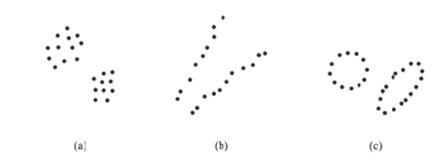
\includegraphics[width=8.5cm]{./Img/Prednaska08/BezUcitele/shluky.png}
	\caption[Typy shluků]{(a)Kompaktní shluky, (b) Podlouhlé shluky, (c) Sférické a elipsoidní shluky}
	\label{fig:shluky}
\end{figure}

\par{Shlukování se využívá v celé škále oborů, například v biologii, ekologii, sociologii, geografii, geologii a grafové teorii. Shlukování je také jednou z nejpřirozenějších mentálních aktivit člověka, který také vjemy a informace klasifikuje do jednotlivých tříd.}
\par{\textbf{Příklady algoritmů:} Sekvenční algoritmy, K-means, Hierarchické algoritmy (aglomerativní, divizní), Fuzzy shlukování, Genetické shlukovací algoritmy, Algoritmy založené na morfologických operacích,...}







%--------------------------------------------------------------------------------------------
\subsubsection*{K-means (MacQueenův algoritmus)}
\par{Jedná se o jeden z nejoblíbenějších a nejrozšířenějších shlukovacích algoritmů. Pro výpočet vzdálenosti mezi dvěma obrazy používá Euklidovu vzdálenost. Mezi jeho hlavní výhody patří jednoduchá implementace a nízká výpočetní náročnost. Mezi nevýhody naopak nutná znalost počtu tříd (shluků), do kterých budeme klasifikovat, a problematický výběr počátečního 'nástřelu' reprezentantů shluků. Algoritmus je vhodný pro kompaktní a sférické shluky a díky jeho rozšířenosti existuje mnoho jeho modifikací (K-methodois, PAM, CLARA, CLARANS). }
\newpage
Nyní bude uveden základní K-means algoritmus a dále podrobněji vysvětlen.

\begin{algorithm}[h!]
	\caption{K-means algoritmus}
	\label{alg:kmeans}
	\begin{algorithmic}[1]
		\State Vstup: Vhodně zvolený odhad reprezentantů $\theta_{j}(0)$ pro j = 1,...,m.
		
		\State for i = 1 to N: rozhodni nejbližšího reprezentanta $\theta_{j}$ pro dané $x_i$, zařaď $x_i$ do shluku j.
		\State for i = 1 to m: aktualizuj parametry: přepočti $\theta_{j}$ jako střední vektor j-tého shluku.
		\State kroky 2 a 3 opakuj dokud se $\theta_j$ ve dvou po sobě jdoucích krocích nezmění.
		\State Výstup: Středy shluků $\theta_j$ + kompletní shlukování pro všechny body

	\end{algorithmic}
\end{algorithm}

\par{V prvním kroku algoritmu je po uživateli požadován počet shluků \textit{m} a vhodný nástřel středů shluků $\theta_j(0)$. Tato část je v praxi často velmi problematická, často je řešena tak, že \textit{j} počátečních nástřelů je zvoleno jako prvních \textit{j} členů dané množiny. Algoritmus se dále snaží minimalizovat následující kritérium 
\begin{equation}
	J(\theta,U) = \sum_{i=1}^{N}\sum_{j=1}^{m} u_{ij}||x_i-\theta_j||^2
\end{equation}  
kde N je počet shluků, m počet bodů množiny, $u_{ij} = 1$ pokud daný bod patří do daného shluku, v opačném případě je  $u_{ij} = 0$. Toho je docíleno tím, že každý bod je zařazen do do shluku od jehož reprezentanta má nejnižší Euklidovu vzdálenost. Po zařazení všech bodů do shluků jsou aktualizování jejich reprezentanti a celý algoritmus je spuštěn znovu. Algoritmus je ukončen ve chvíli, kdy reprezentanti nejsou změněni ve dvou po sobě jdoucích cyklech.}



%--------------------------------------------------------------------------------------------
\subsubsection*{Hierarchické algoritmy}
\par{Na rozdíl od algoritmu K-means nepotřebujeme znát dopředu finální počet shluků. Jejich hlavní výhodou je, že po uživateli nejsou vyžadovány žádné počáteční parametry (na rozdíl od algoritmu K-means nepotřebujeme znát dopředu finální počet shluků, atd). Výsledkem těchto algoritmů není jen jediné shlukování, nýbrž jejich sekvence. Hierarchické algoritmy se dělí na dvě základní skupiny a to \textbf{aglomerativní} a \textbf{divizní}.  }
\par{Základní myšlenkou aglomerativních algoritmů je v každém iteračním kroku spojit dva shluky (body) s nejvyšším kritériem podobnosti (nejnižší vzdáleností) do jediného shluku. Jestliže jsou dva vektory (obrazy) spojeny do stejného shluku v kroku \textit{t}, setrvají ve stejném shluku až do konce algoritmu. To znamená, že na počátku každý bod tvoří vlastní shluk, tyto body jsou postupně spojovány do větších, až v posledním kroku algoritmu zbude pouze jediný shluk obsahující všechny prvky množiny.}
\par{Hierarchické algoritmy jsou vhodné pro kompaktní a podlouhlé shluky. Jejich výsledkem je, jak již bylo řečeno, sekvence shlukování. Tuto sekvenci lze přehledně zobrazit pomocí \textbf{dendogramu}. Jejich hlavní nevýhodou je nutnost vybrat správné shlukování ze získané sekvence. To lze zvolit pomocí několika přístupů, mezi ně patří například délka života shluků či definice maximálního prahu, po jehož překročení již shluky nebudou spojeny.}
\par{Divizní algoritmy postupují přesně opačným způsobem než aglomerativní, takzvaně v~prvním kroku jsou všechny body členy jediného shluku a tento shluk je dále dělen až do chvíle, kdy každý bod je ve svém shluku sám. Nejsou příliš využívány vzhledem k jejich vysoké výpočetní náročnosti.}








%--------------------------------------------------------------------------------------------












\newpage















%-------ADABOOST----------------------------------------------------------------------------
%-LUKAS-BURES-
\section{AdaBoost}
\label{sec:07_AdaBoost}

\par{Adaptive Boosting (AdaBoost nebo AB) je algoritmus klasifikace a má tyto zajímavé vlastnosti:
\begin{itemize}
	\item AdaBoost je lineární klasifikátor se všemi jeho potřebnými vlastnostmi.
	\item Výstup AdaBoost konverguje k logaritmu věrohodnosti ( output converges to the logarithm of likelihood ratio).
	\item AdaBoost dobře zobecňuje.
	\item AdaBoost je příznakový selektor se zásadovou strategií (minimalizuje horní mez empirické chyby).
	\item AdaBoost je podobný sekvenčnímu rozhodování (produkuje posloupnost postupně složitějších klasifikátorů).
\end{itemize}}

\subsection*{AdaBoost}
\par{AdaBoost je algoritmus sestavující \uv{silný} klasifikátor jako lineární kombinaci \uv{slabých} klasifikátorů.}

\par{\textbf{Příklad:} Nechť existuje imaginární závislý sázkař na dostihy, který se řídí nepsanými pravidly pro stanovení \textit{výhry} / \textit{prohry}: nejlepší kurz, nejrychlejší čas daného koně na kolo, nejvíce výher v~poslední době (například za poslední měsíc). Z~uvedeného lze konstatovat, že je velmi složité určit (na základě kombinace všech možných příznaků) na koho má gambler vsadit.}

\par{\textbf{Příklad:} Rozhodování o přijmutí na FAV, jedná se o~binární klasifikaci (klasifikace do dvou tříd) \textit{Přijat} / \textit{Odmítnut}. V~tabulce \ref{tab:prijetiNaFAV} jsou uvedeny, jak kvalitativní, tak kvantitativní trénovací vzorky.}
\begin{table}[!ht]
	\centering
	\begin{tabular}{|c|c|c|c|c|c|c|}
		\hline
		{ID} & {Jméno} & {Rozhodnutí} & {Kraj} & {Pohlaví} & {Dobrý v} & {Dobrý ve}\\
		{} & {} & {} & {} & {} & {matematice} & {sportu}\\
		\hline
		\hline		
		{1} & {Andrea} & {Přijat} & {Západočeský} & {Ž} & {Ano} & {Ne}\\		
		{2} & {Pepa} & {Přijat} & {Severočeský} & {M} & {Ano} & {Ne}\\
		{3} & {Lukáš} & {Odmítnut} & {Severomoravský} & {M} & {Ne} & {Ne}\\
		{4} & {Petr} & {Odmítnut} & {Středočeský} & {M} & {Ne} & {Ano}\\
		{5} & {Lucie} & {Odmítnut} & {Západočeský} & {Ž} & {Ano} & {Ano}\\
		{6} & {Ota} & {Přijat} & {Středočeský} & {M} & {Ne} & {Ano}\\
		{7} & {Žofie} & {Odmítnut} & {Východočeský} & {Ž} & {Ne} & {Ne}\\
		{8} & {Jaroslav} & {Odmítnut} & {Západočeský} & {M} & {Ne} & {Ano}\\
		{9} & {Jan} & {Odmítnut} & {Západočeský} & {M} & {Ne} & {Ano}\\
		{10} & {Marek} & {Přijat} & {Jihočeský} & {M} & {Ano} & {Ne}\\
		\hline
	\end{tabular}
	\caption{Imaginární výsledky přijmutí na FAV.}
	\label{tab:prijetiNaFAV}
\end{table}

\par{Je jednoduché vymyslet klasifikátor, který bude správně klasifikovat trénovací data lépe než náhodně (úspěšnost klasifikace, při problému klasifikace do dvou tříd, musí být ostře větší než $50\%$). Slabý klasifikátor by bylo možné sestrojit z podmínky, pokud je uchazeč dobrý v~matematice tak predikuj \textsf{Přijat}. Na druhou stranu je velmi složité najít jediný silný klasifikátor, který velmi přesně predikuje výslednou klasifikaci.}


\subsubsection*{Co je slabý klasifikátor}
\par{Pro každé rozdělení pravděpodobnosti dané polynomiálním počtem vzorků a polynomiálním časem může být nalezen takový klasifikátor, který má obecně lepší chybu než při náhodné klasifikaci. Tedy, chyba 
\begin{equation}
	\varepsilon < 0.5,
\end{equation}
což lze také zapsat jako $\gamma > 0$ pro obecnou chybu ($0.5 - \gamma$).}

\par{Předpokladem je, že lze zkonstruovat slabý klasifikátor, tak aby trvale klasifikoval do správné třídy s~lepší než $50\%$ pravděpodobností.}

\par{Vzhledem k~tomuto předpokladu je možné využít mnoho slabých klasifikátorů pro sestavení jednoho silného klasifikátoru, který bude správně klasifikovat $99-100\%$ vstupních vzorků.}


\subsubsection*{AdaBoost algoritmus}
\par{Nyní bude představen diskrétní AdaBoost algoritmus a následně bude vysvětlen podrobněji.}

\par{Nechť existuje trénovací sada dat $S = \{ \left( \bm{x}_1, y_1 \right), \left( \bm{x}_2, y_2 \right), \cdots , \left( \bm{x}_N, y_N \right) \}$, kde $y_i \in \{ -1, 1\}$ je výstupní klasifikace a~$\bm{x}_i \in \bm{X}$ je vstupní příznakový vektor reálného objektu.}

\begin{algorithm}
	\caption{Diskrétní AdaBoost algoritmus}
	\label{alg:AdaBoost}
	\begin{algorithmic}[1]
		\State Vstup: $S = \{ \left( \bm{x}_1, y_1 \right), \left( \bm{x}_2, y_2 \right), \cdots , \left( \bm{x}_N, y_N \right) \}$. Počet iterací $T$.
		\State Inicializace: $d_n^{\left( 1 \right)} = \frac{1}{N}$ pro všechny $n = 1,\cdots, N$.
		\For{$t = 1, \cdots , T$}
			\State Natrénuj klasifikátor vzhledem k vážené množině vzorků $\{S, \bm{d}^{\left( \bm{t} \right)}\}$ a získej hypotézu $h_t : \bm{x} \mapsto \{ -1, +1\}$, tj. $h_t = L \left( S, \bm{d}^{\left( \bm{t} \right)} \right)$.
			\State Vypočti váženou chybu trénovací sady $\varepsilon_t$ pro hypotézu $h_t$: 
				\begin{equation}
					\varepsilon_t = \sum_{n = 1}^{N} d_n^{\left( t \right)} \bm{I} \left( y_n \neq h_t \left( x \right)_n \right).
				\end{equation}
			\State Nastav:
				\begin{equation}
					\alpha_t = \frac{1}{2} \log \frac{1 - \varepsilon_t}{\varepsilon_t}.
				\end{equation}
			\State Aktualizuj váhy:
				\begin{equation}
					d_n^{\left( t + 1 \right)} = \frac{d_n^{\left( t \right)} \cdot e^{- \alpha_t y_n h_t \left( x_n \right)}}{Z_t},
				\end{equation}
				kde $Z_t$ je normalizační konstanta taková, že platí $\sum_{n =1}^{N} d_n^{\left( t + 1 \right)}= 1$.
			\If{$\varepsilon_t = 0$ \textbf{or} $\varepsilon_t \geq \frac{1}{2}$}
				\State Ukonči a nastav: $T = t - 1$
			\EndIf
		\EndFor
		\State Výstup: $f_T \left( x \right) = \sum_{t = 1}^{\top} \frac{\alpha_t}{\sum_{r = 1}^{T} \alpha_r} h_t \left( x \right)$.
	\end{algorithmic}
\end{algorithm}


\subsubsection*{Vysvětlení diskrétního AdaBoost algoritmu}

\par{AdaBoost je agresivní algoritmus, který vybere jeden slabý klasifikátor v každém kroku. Váhy $\bm{d}^{\left( \bm{t} \right)} = \left( d_1^{\left( t \right)}, \cdots , d_N^{\left( t \right)} \right) $ jsou přiřazeny k datům v kroku $t$ a slabý klasifikátor $h_t$ je založen na $\bm{d}^{\left( \bm{t} \right)}$. Tyto váhy jsou aktualizovány každou iteraci. Váhy se zvětšují pro vzorky, které byly špatně klasifikovány v předchozí iteraci.}

\par{Váhy jsou inicializovány uniformě: $d_n^{\left( 1 \right)} = \frac{1}{N}$ pro obecnou verzi AdaBoost algoritmu. Pro odhad, pokud jsou nějaké vzorky klasifikovány dobře nebo špatně, slabý klasifikátor produkuje váženou empirickou chybu definovanou následovně
\begin{equation}
	\varepsilon_t = \sum_{n = 1}^{N} d_n^{\left( t \right)} \bm{I} \left( y_n \neq h_t \left( x \right)_n \right).
\end{equation}}

\par{Když algoritmus vybere nejlepší hypotézu $h_t$, tak její váhy $\alpha_t = \frac{1}{2} \log \frac{1 -\varepsilon_t}{\varepsilon_t}$ jsou vypočteny tak, aby minimalizovaly ztrátovou funkci. Jedna z možných ztrátových funkcí používaných v AdaBoost je 
\begin{equation}
	G^{AdaBoost} \left( \alpha \right) = \sum_{n = 1}^{N} e^{- y_n \left( \alpha h_t \left( x_n \right) + f_{n - 1} \left( x_n \right) \right)},
\end{equation}
kde
\begin{equation}
	f_{t - 1} \left( x \right) = \sum_{r = 1}^{t - 1} \alpha_r h_r \left( x_n \right).
\end{equation}}

\par{Iterační smyčka je zastavena pokud empirická chyba $\varepsilon_t = 0$ nebo $\varepsilon_t \geq \frac{1}{2}$. Pokud je $\varepsilon_t = 0$, tak je klasifikace optimální. Pokud $\varepsilon_t \geq \frac{1}{2}$, tak klasifikátor přestal respektovat podmínku slabých klasifikátorů a algoritmus AdaBoost nemůže fungovat.}

\par{Všechny slabé hypotézy, které jsou vybrány do stavu $h_t$ jsou lineárně zkombinovány následovně
\begin{equation}
	f_T \left( x \right) = \sum_{t = 1}^{\top} \frac{\alpha_t}{\sum_{r = 1}^{\top} \alpha_r} h_t \left( x \right).
\end{equation}}

\par{Výsledný klasifikátor je založený na jednoduchém prahování, které rozhodne o tom, zda bude vzorek přijat nebo odmítnut.}


\subsubsection*{Vliv slabých klasifikátorů}
\par{V každé iteraci AdaBoost vytvoří slabé klasifikátory založené na vážených vzorcích. Nyní bude diskutována výkonnost těchto slabých klasifikátorů založených na opětovném vážení vzorků. Pro pozorování vlivu slabých klasifikátorů nejprve nutné definovat několik základních nástrojů.}

\par{Základní klasifikátor: Nechť $\bm{d} = \left( d_1, \cdots , d_n \right)$ je váha (pravděpodobnost) vzorků $S$. Nechť $S_+$ je podmnožina vzorků, které jsou označeny kladně a podobně pro $S_-$. Dále $D_+ = \sum_{n:y_n = +1} d_n$ a podobně pro $D_-$. Základní klasifikátor $f_{BL}$ (index $BL$ značí \uv{Base Line}) je definován jako
\begin{equation}
	f_{BL} \left( x \right) = sign \left( D_+ - D_- \right), \quad \forall x.
\end{equation}
Tedy predikuje $+1$ pokud $D_+ \geq D_-$ jinak $-1$. Je okamžitě zřejmé, že pro všechny váhy $\bm{d}$ je chyba základního klasifikátoru nejvýše $\frac{1}{2}$.}

\par{S touto definicí je možné lépe definovat slabý klasifikátor: Slabý klasifikátor vzorků $S$, pokud jsou dány váhy $\bm{d}$ vzorků $S$, je schopen dosáhnout vážené chyby klasifikace, která je striktně menší než $\frac{1}{2}$.}

\par{Klíčová vlastnost Boosting algoritmu je splnění podmínky pro slabý klasifikátor, který je potřeba pro to, aby celkový algoritmus fungoval správně. Vážená empirická chyba každého slabého klasifikátoru musí být striktně menší než $\frac{1}{2} - \frac{1}{2} \gamma$, kde $\gamma$ je parametr určující odchylku od od základního klasifikátoru představeného dříve. Je uvažován slabý binární klasifikátor $h$, vzhledem k množině vzorků $S = \{ \left( x_n , y_n \right) \}_{n = 1}^{N}$, kde pro každou dvojici $\left( x_n, y_n\right)$ existuje nezáporná váha $d_n$. Pak je požadováno, aby 
\begin{equation}
	\varepsilon_t \left( h_t, \bm{d} \right) = \sum_{n = 1}^{N} d_n \bm{I} \left( y_n \neq h \left( x \right)_n \right) \leq \frac{1}{2} - \frac{1}{2} \gamma, \quad \left( \gamma > 0 \right).
	\label{eq:AdaBoostEmpirickaChyba}
\end{equation}}

\par{Pro nějaké slabé klasifikátory nemusí existovat $\gamma > 0$, která respektuje předchozí podmínku aniž by porušila některé podmínky týkající se dat.}

\par{Příklad možného nalezení pozitivní $\gamma$, která respektuje podmínku empirické chyby \ref{eq:AdaBoostEmpirickaChyba}. Předpokladem je mapování $f$ z binární krychle $\bm{X} = \{ +1 , -1\}^d$ do $\bm{Y} = \{ + 1 , -1\}$ a~dále pozitivní labely $y_n$, které jsou dány $y_n = f \left( x_n \right)$. Funkce $f$ je aproximována binární hypotézou $h_t$ patřící do $\bm{H}$. Nechť $H$ je třída binárních hypotéz a nechť $D$ je rozložení nad $\bm{X}$. Korelace mezi $f$ a $H$ s respektováním $D$ je dána $C_{H, D}\left( f \right) = \sup_{h \in H} \bm{E}_D \{ f\left( x \right) h \left( x \right) \}$. Rozložení bez korelace mezi $f$ a $H$ je dáno $C_H \left( f \right) = \inf_D C_{H,D} \left( f \right)$. To může být dokázáno, pokud $T > 2 \cdot \log \left( 2 \right) d C_H \left( f \right)^{-2}$, pak $f$ může být reprezentována přesně jako
\begin{equation}
	f \left( x \right) = sign \left( \sum_{t = 1}^{T} h_t \left( x \right) \right).
\end{equation}}

\par{Jinými slovy, pokud je $H$ silně korelována s cílovou funkcí $f$, pak $f$ může být přesně reprezentována jako kombinace malých čísel funkce z $H$. Proto poté pro dostatečně velký počet iterací může být očekáváno, že se empirická chyba bude blížit nule.}

\par{Tento příklad ukázal binární klasifikaci s dvěma lineárně oddělitelnýma třídami. Ve více obecném případě můžou být třídy silně se překrývající, proto je nutné využít pokročilejší nástroje jako vytvořit pravidla týkající se slabých klasifikátorů.}
\pagebreak

\begin{table}[!ht]
	\centering
	\begin{tabular}{| p{7.5cm} | p{7.5cm} |}
		\hline
		{\textbf{Výhody AdaBoost algoritmu}} & {\textbf{Nevýhody AdaBoost algoritmu}}\\
		\hline
		\hline
		{Rychlost. ~} & {Slabé klasifikátory, které jsou současně komplexní vedou k~přetrénování.}\\
		\hline
		{Prokazatelná efektivita vzhledem k~předpokladu slabých klasifikátorů.} & {Pokud jsou slabé klasifikátory příliš slabé může vznikat \uv{low margin} problém i~problém přetrénování.}\\
		\hline
		{Není potřeba volit žádný parametr (vyjma počtu iterací $T$).} & {Z empirických důkazů bylo ukázáno, že AdaBoost algoritmus je náchylný na uniformní šum.}\\
		\hline
		{Není potřebná žádná apriorní informace.} & {}\\
		\hline
		{Jednoduchá implementace.} & {}\\
		\hline
		{Univerzálnost.} & {}\\
		\hline
	\end{tabular}
	\label{tab:AdaBoostVyhodyNevyhody}
\end{table}




\newpage
%------KASKADNI-ADABOOST----------------------------------------------------------------------
%-LUKAS-BURES-
\section{Kaskádní AdaBoost}
\label{sec:AdaBoostKaskadniAdaBoost}

\par{Je možné vybrat malé množství dobře odlišitelných příznaků a zkombinovat je do jednoho silného klasifikátoru, nicméně je potřeba představit několik hlavních myšlenek pro snížení výpočetního času. Rozšíření spočívá v tvorbě kaskády klasifikátorů, která navíc může dosahovat lepší klasifikační přesnosti. Tedy snaží se minimalizovat počet false negativ klasifikací namísto klasického trénování chyby, což představuje hlavní myšlenku, která bude dále sloužit pro vytvoření kaskády klasifikátorů.}

\par{Princip bude vysvětlen na praktickém příkladě hledání obličejů v obrázku.}

\subsubsection*{Proč je to tak efektivní?}
\par{Princip spočívá v rychlém odmítnutí většiny negativních okének a ponechání co nejvíce pozitivních. Následně se využije více citlivějších (menších) podokének s více komplexnějšími klasifikátory. V první fázi kaskády, která obsahuje pouze několik málo příznaků se většinou dosahuje velmi vysokého detekčního poměru (kolem $100\%$), avšak na úkor false positive (přibližně $40\%$). Je zřejmé, že pro výslednou klasifikaci je takový počet chyb nepřijatelný. Proto se v případě problému detekce obličejů kombinuje mnoho za sebou navazujících klasifikátorů, což vede k více a více diskriminativní klasifikaci jejímž výsledkem je detekce obličejů ve scéně.}

\par{Tuto kaskádní strukturu lze přirovnat k~degenerovanému rozhodovacímu stromu. Pokud je podokénko klasifikováno jako pozitivní v~jednom stupni, tak postupuje dále v~kas\-ká\-dě a~je ověřováno v~každém dalším stupni znovu. Takto se pokračuje dále dokud není podokénko označeno negativně, nebo je po ověření poslední vrstvou prohlášeno za pozitivní (obsahující tvář). Na Obr.~\ref{fig:KaskadniAdaBoost} je tento proces naznačen.
\begin{figure}[!ht]
	\centering
	%trim option's parameter order: left bottom right top
	%\fbox{
	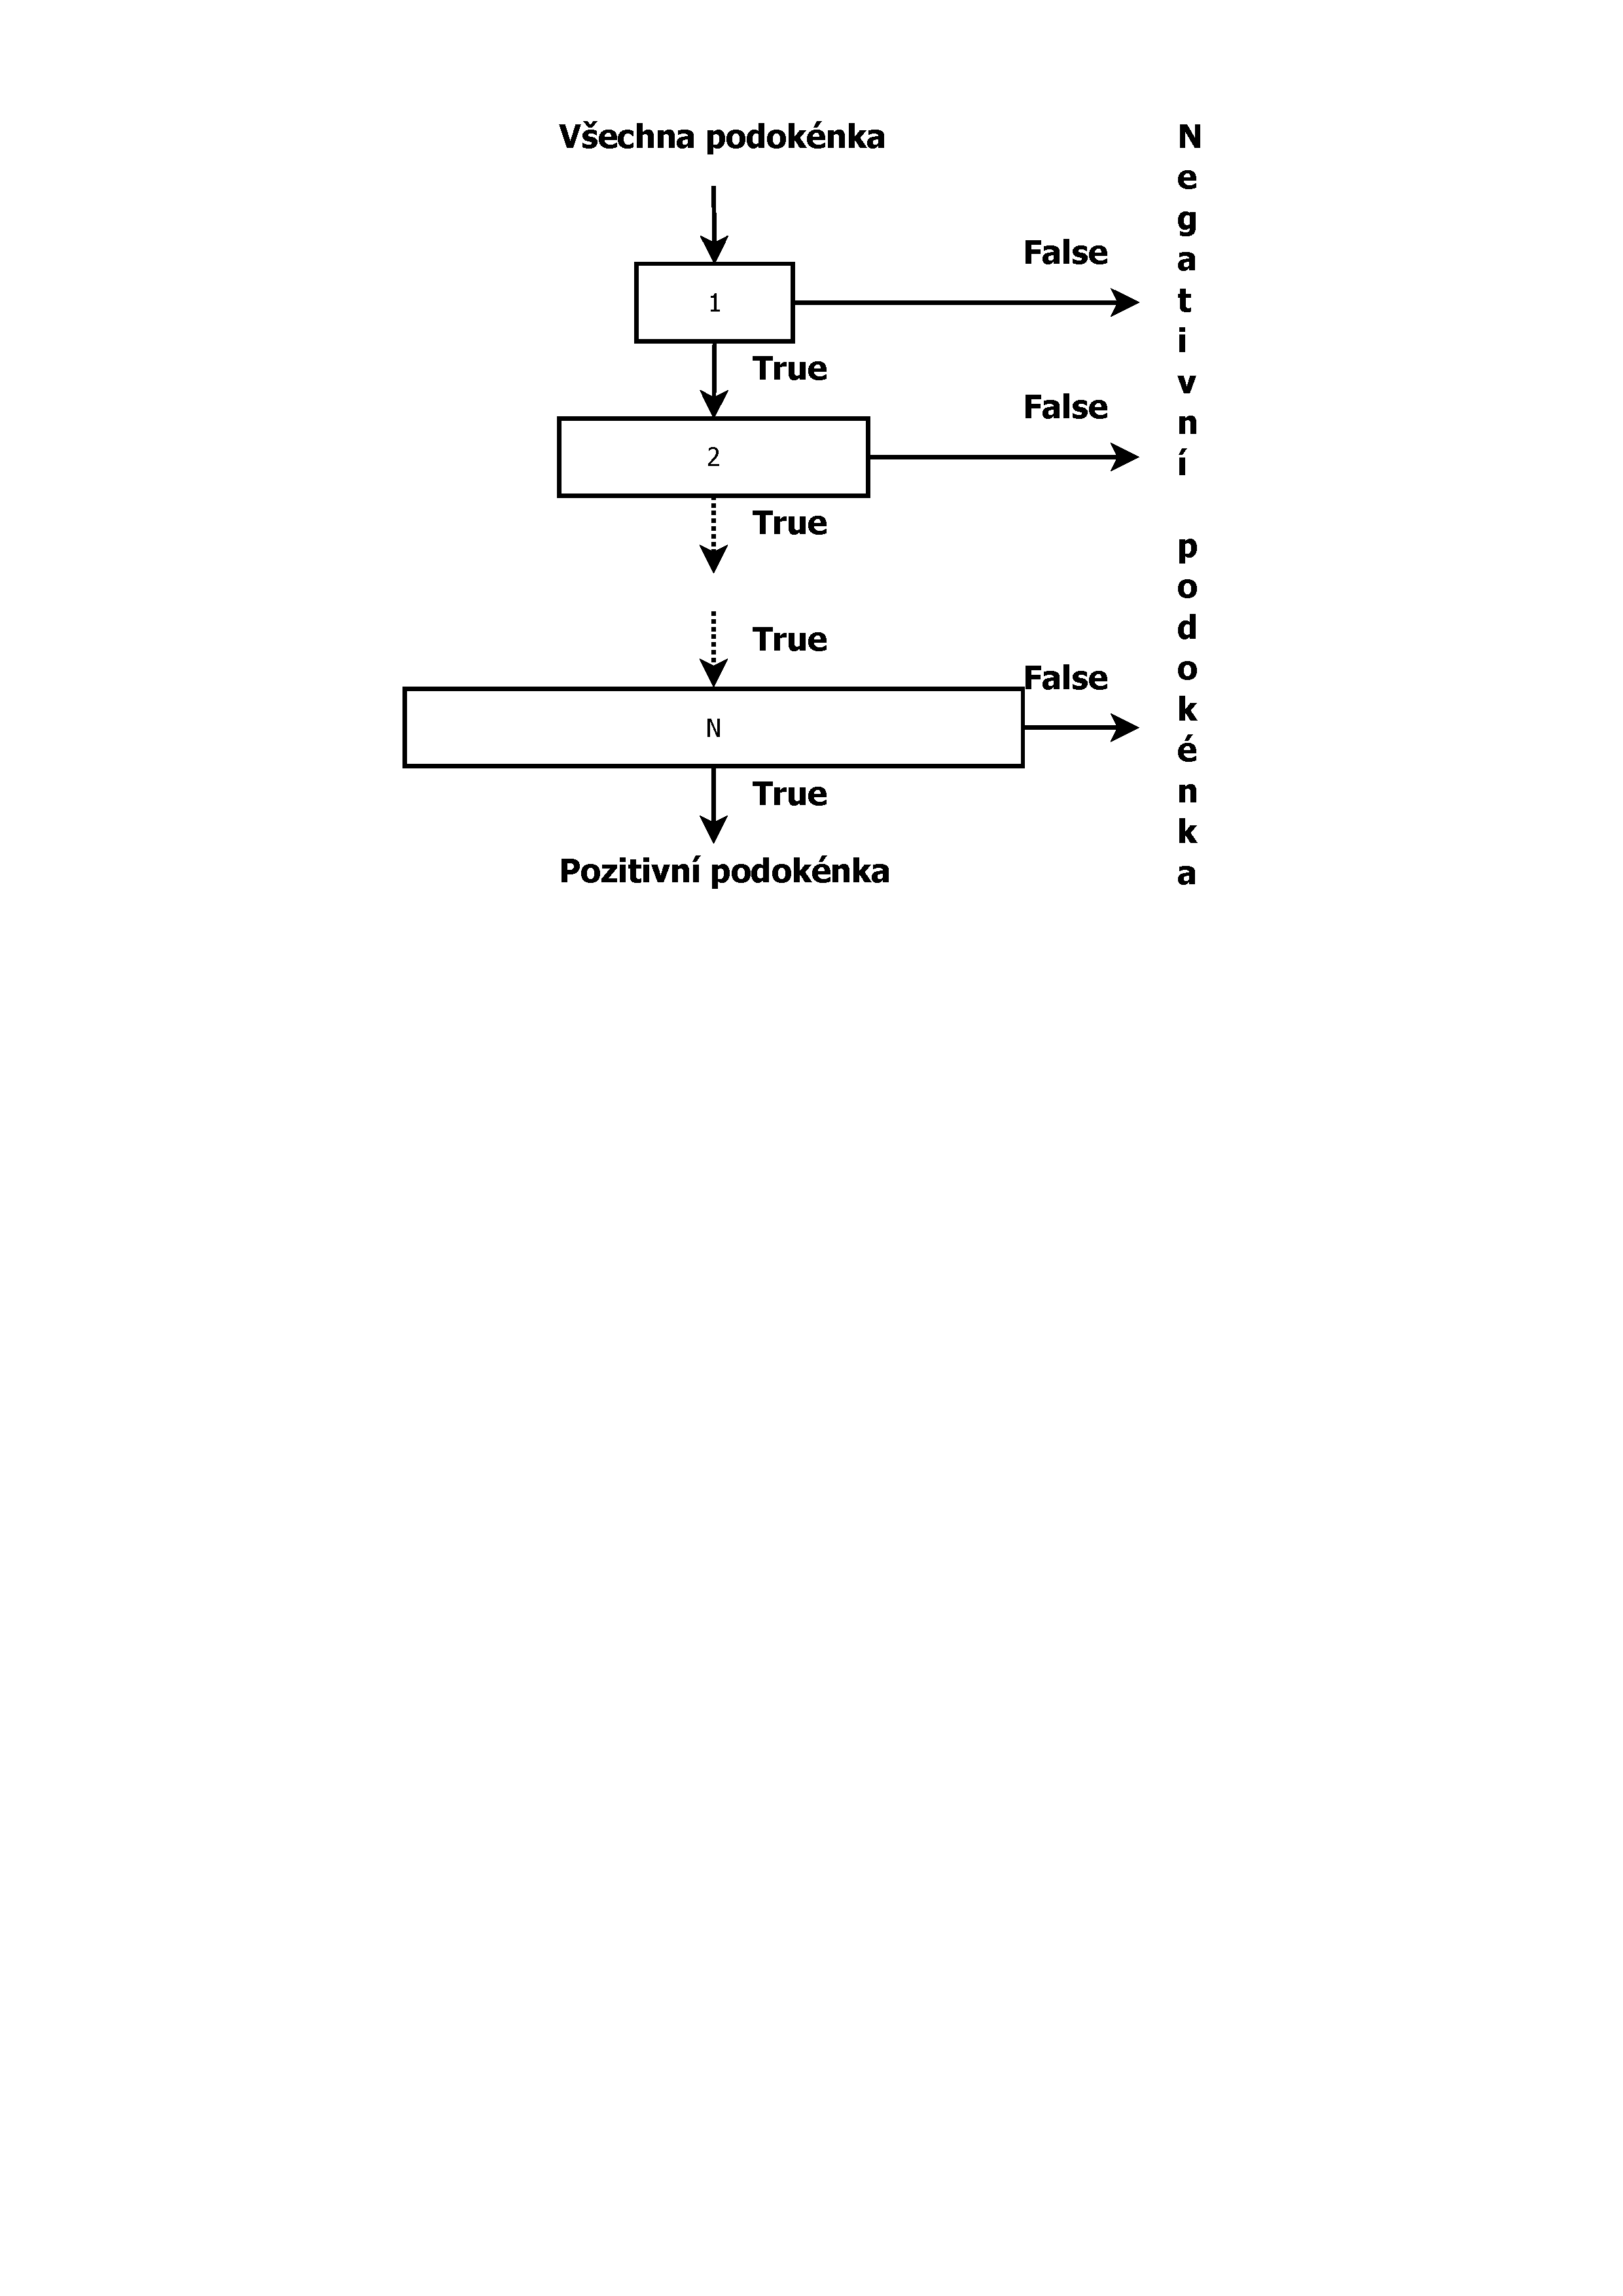
\includegraphics[width = 0.4\textwidth, trim = 10cm 36cm 10cm 3cm]{./Img/Prednaska08/KaskadniAdaBoost/KaskadaAdaBoost.pdf}
	\caption{Schématický popis kaskádní detekce. Série klasifikátorů je aplikována na každé podokénko. Počáteční klasifikátor eliminuje velký počet negativních vzorků s malým processingem. Další vrstvy eliminují další negativní vzorky, tudíž je potřeba dalšího výpočetního času. Po několika stupních processingu je počet podokének radikálně redukován. Vzorky, které jsou klasifikovány jako pozitivní v posledním stupni jsou definitivně označeny jako pozitivní.}
	\label{fig:KaskadniAdaBoost}
\end{figure}}



\subsubsection*{Tvorba více konzistentních klasifikátorů}
\par{Byla definována kaskáda jako množina na sebe navazujících klasifikátorů. První klasifikátor je velmi jednoduchý, ale postupem v kaskádě nabývá na složitosti.}

\par{V poslední vrstvě má klasifikátor více příznaků než v první. AdaBoost algoritmus generuje chybu trénování, která klesá teoreticky exponenciálně v závislosti na počtu iterací. Pokud je více příznaků (AdaBoost algoritmus běží více iterací) výsledný klasifikátor je více diskriminativní mezi pozitivními a negativními vzorky. Jinými slovy lze říci, že je klasifikátor \uv{silnější} než v případě kdy má k dispozici méně příznaků (běží menší počet iterací).}

\par{Další důležitou věcí kaskádního AdaBoost algoritmu je volba trénovací množiny. V~kaž\-dé vrstvě (učícím se kroku, iteraci) je $i$-tý klasifikátor testován na testovací množině negativních vzorků. Všechny špatně klasifikované negativní vzorky jsou předány dále do $\left( i + 1 \right)$-tého klasifikátoru, který se tedy musí zaměřit na složitější vzorky. Snaha spočívá v donucení následujícího klasifikátoru, aby měl poměr nalezených false positive vzorků menší než předchozí klasifikátor.}



\subsubsection*{Trénování kaskádního AdaBoost algoritmu}
\par{Nechť $F$ je míra detekovaných false positive vzorků kaskádního klasifikátoru, $K$ je počet klasifikátorů a $f_i$ je míra false positive vzorků $i$-tého klasifikátoru. Pro trénovanou kaskádu klasifikátorů je $F$ dáno jako
\begin{equation}
	F = \prod_{i = 1}^K f_i,
\end{equation}
následně míra detekce může být vypočtena jako
\begin{equation}
	D = \prod_{i = 1}^K d_i,
\end{equation}
kde $d_i$ je míra detekce $i$-tého klasifikátoru na vzorcích procházející daným klasifikátorem.}

\par{Počet příznaků, které musí byt hledány v reálném obrázku (například při hledání obličeje) nezbytný pravděpodobnostní proces. Většina podokének projdou kaskádou jedním nebo několika klasifikátory než jsou vyhodnoceny jako negativní vzorek a jen velmi malá část vzorků je na konci označena jako pozitivní vzorek. Chování tohoto procesu je závislé na pravděpodobnostním rozdělení obrázků v trénovací sadě. Hlavním nástrojem pro měření výkonu klasifikátorů je míra pozitivních vzorků na konci kaskády. Vzhledem k~počtu vrstev v~kaskádě $K$ je míra pozitivních vzorků v $i$-té vrstvě (klasifikátoru) označena $p_i$. Nechť $n_i$ je počet příznaků v $i$-té vrstvě. Očekávaný počet příznaků, který je ověřován, je dán 
\begin{equation}
	N = n_0 + \sum_{i = 1}^{K} \left( n_i \prod_{j < i} p_i \right).
\end{equation}
Jen několik málo příkladů je klasifikováno jako hledané objekty (obličeje), což je také důvod, proč je míra pozitivních vzorků přibližně rovna míře false positive vzorků.}


\newpage

\par{Struktura kaskádního AdaBoost algoritmu vyžaduje znalost tří parametrů
\begin{enumerate}
	\item Celkový počet klasifikátorů $K$.
	\item Počet příznaků $n_i$ v $i$-té vrstvě.
	\item Práh $\theta_i$ v $i$-té vrstvě.
\end{enumerate}
Nalezení těchto optimálních parametrů je obtížné, za předpokladu, že je nutné minimalizovat výpočetní čas celé klasifikace. Princip spočívá ve zvýšení počtu příznaků a počtu vrstev dokud není dosažená stanovená úspěšnost klasifikace.}

\par{Vzhledem k minimální přijatelné míře $f_i$ (false positive míra pro $i$-tou vrstvu) a $d_i$ (míra detekce pro $i$-tou vrstvu) je míra detekce $d_i$ dosažena za pomoci snižování prahu $\theta_i$, což přímo ovlivňuje $f_i$. Počet příznaků $n_i$ v $i$-té vrstvě je zvyšován dokud není dosaženo $f_i$. Obecný kaskádový AdaBoost algoritmus je naznačen v algoritmu \ref{alg:KaskadniAdaBoostUceni} a bude diskutován níže.}

\par{Jeden z hlavních faktorů efektivity kaskádového algoritmu je správa trénovací množiny během učení. Většinou je trénovací množina použita pro první vrstvu následně každou iteraci je aktuální klasifikátor ověřován na validační množině. Je velmi nevhodné ověřovat úspěšnost klasifikace na trénovací množině, jelikož bude pro tuto množinu bude úspěšnost vyšší. V každé další vrstvě je trénovací množina negativních vzorků znovu inicializována. Když je dosaženo $F_i$ a $D_i$ pro $i$-tou vrstvu, tak je aktuální model testován na velké množině negativních vzorků, které jsou zvoleny náhodně. Mnoho false positive vzorků je vloženo do trénovací sady negativních vzorků v $i-1$-té vrstvě. Nová trénovací množina negativních vzorků je vytvořena ze vzorků, které byly špatně detekovány v $i$-té vrstvě, tedy následující $i+1$-tá vrstva je trénována na vzorcích, které jsou pro předešlo vrstvu \uv{složité}. Tedy, čím dále v kaskádě se klasifikátor nachází, tím lépe dokáže klasifikovat mezi pozitivními a negativními vzorky (podokýnky obsahujícími lidské tváře).}

\newpage

\begin{algorithm}[!ht]
	\caption{Učení kaskádního AdaBoost algoritmu}
	\label{alg:KaskadniAdaBoostUceni}
	\begin{algorithmic}[1]
		\State Vstup: $f$ maximální přijatelná míra false positive pro každou vrstvu, $d$ minimální přijatelná míra detekce pro každou vrstvu, $F_{target}$ počet false positive na konci procesu, $P$ množina pozitivních vzorků,	$N$ množina negativních vzorků.
		\State Inicializace: $F_0 = D_0 = 1$, $i = 0$ číslo aktuální vrstvy.
		\While{$F_i > F_{target}$}
			\State $i = i + 1$
			\State $n_i = 0$
			\State $F_i = F_{i - 1}$

			\While{$F_i > f \cdot F_{i - 1}$}
				\State $n_i = n_i + 1$
				\State Natrénuj AdaBoost klasifikátor (algoritmus \ref{alg:AdaBoost}) s $P$ a $N$ jako trénovací množinou.
				\State Vypočti $F_i$ a $D_i$ pro aktuální klasifikátor na základě validační množiny.
				\State Snižuj práh klasifikátoru dokud není poměr $i$-tého klasifikátoru alespoň 
					\begin{equation}
						d \cdot \frac{D_{i - 1}}{D_i} \geq D_{i - 1} \cdot d
					\end{equation}
			\EndWhile			
			
			\State Smaž negativní vzorky trénovací množiny.
			\If{$F_i > F_{target}$}
				\State Ověř aktuální kaskádu klasifikátorů na množině negativních vzorků a vlož nějaké špatně detekované vzorky do množiny $N$.
			\EndIf
		\EndWhile
	\end{algorithmic}
\end{algorithm}

\newpage



























%-------SVM--------------------------------------------------------------------------------------
%-PETR-ZIMMERMANN-
\section{SVM}
\label{sec:07_SVM}
\par{Tato metoda hledá v prostoru nejširší možný pruh, který rozděluje množinu vektorů
do~dvou nadrovin. Nadrovina je následně popsána pomocí vektorů ležících nejblíže její hranice, kterých je obvykle malý počet a nazývají se support vectors. Tyto vektory daly za vznik názvu celé metody SVM (z ang. \textit{Support Vectors Machine}). Princip klasifikační metody SVM bude nejprve vysvětlen na případu jednoznačně oddělitelné množiny (lineárně separovatelná množina) vektorů a následně se text zaměří na mnohem obecnější případ množiny, kterou nelze jednoznačně rozdělit (nelineárně separovatelná množina) do~dvou tříd.}


\subsubsection*{Lineárně separovatelná množina}
\par{Nechť $\bm{x}_i,i=1,2,\ldots,N$, jsou vektory tvořící trénovací množinu $X$. Vektory náleží do jed\-né ze dvou tříd $\omega_1,\omega_2$ a jsou lineárně separovatelné. To znamená, že existuje parametr $\omega$, pro který platí
\begin{eqnarray}
	\nonumber
	&\bm{\omega}^{\top} \bm{x} > 0,&\textrm{pro}~\forall \bm{x} \in \omega_1,\\
	\nonumber
	&\bm{\omega}^{\top} \bm{x} < 0,&\textrm{pro}~\forall \bm{x} \in \omega_2.
\end{eqnarray}
Jinými slovy, úkolem klasifikační metody je nalézt nadrovinu $g\left( \bm{x} \right)$
\begin{equation}
	g\left( \bm{x} \right) = \bm{\omega}^{\top} \bm{x} + \omega_0 = 0,
	\label{eq:SVMhyperplane}
\end{equation}
která rozděluje vektory $\bm{x}_i$ do příslušných tříd. Koeficient $\omega_0$ z předpisu \ref{eq:SVMhyperplane} je nulový pouze v případě že nadrovina prochází počátkem souřadnicového systému. Jak je patrné z Obr. \ref{fig:SVM01}, rozdělujících nadrovin je obvykle celá řada. Úkolem klasifikační metody SVM je zvolit takovou, která minimalizuje chybu klasifikace tím, že má maximální možný odstup od obou tříd.
\begin{figure}[!ht]
	\centering
	%trim option's parameter order: left bottom right top
	%\fbox{
	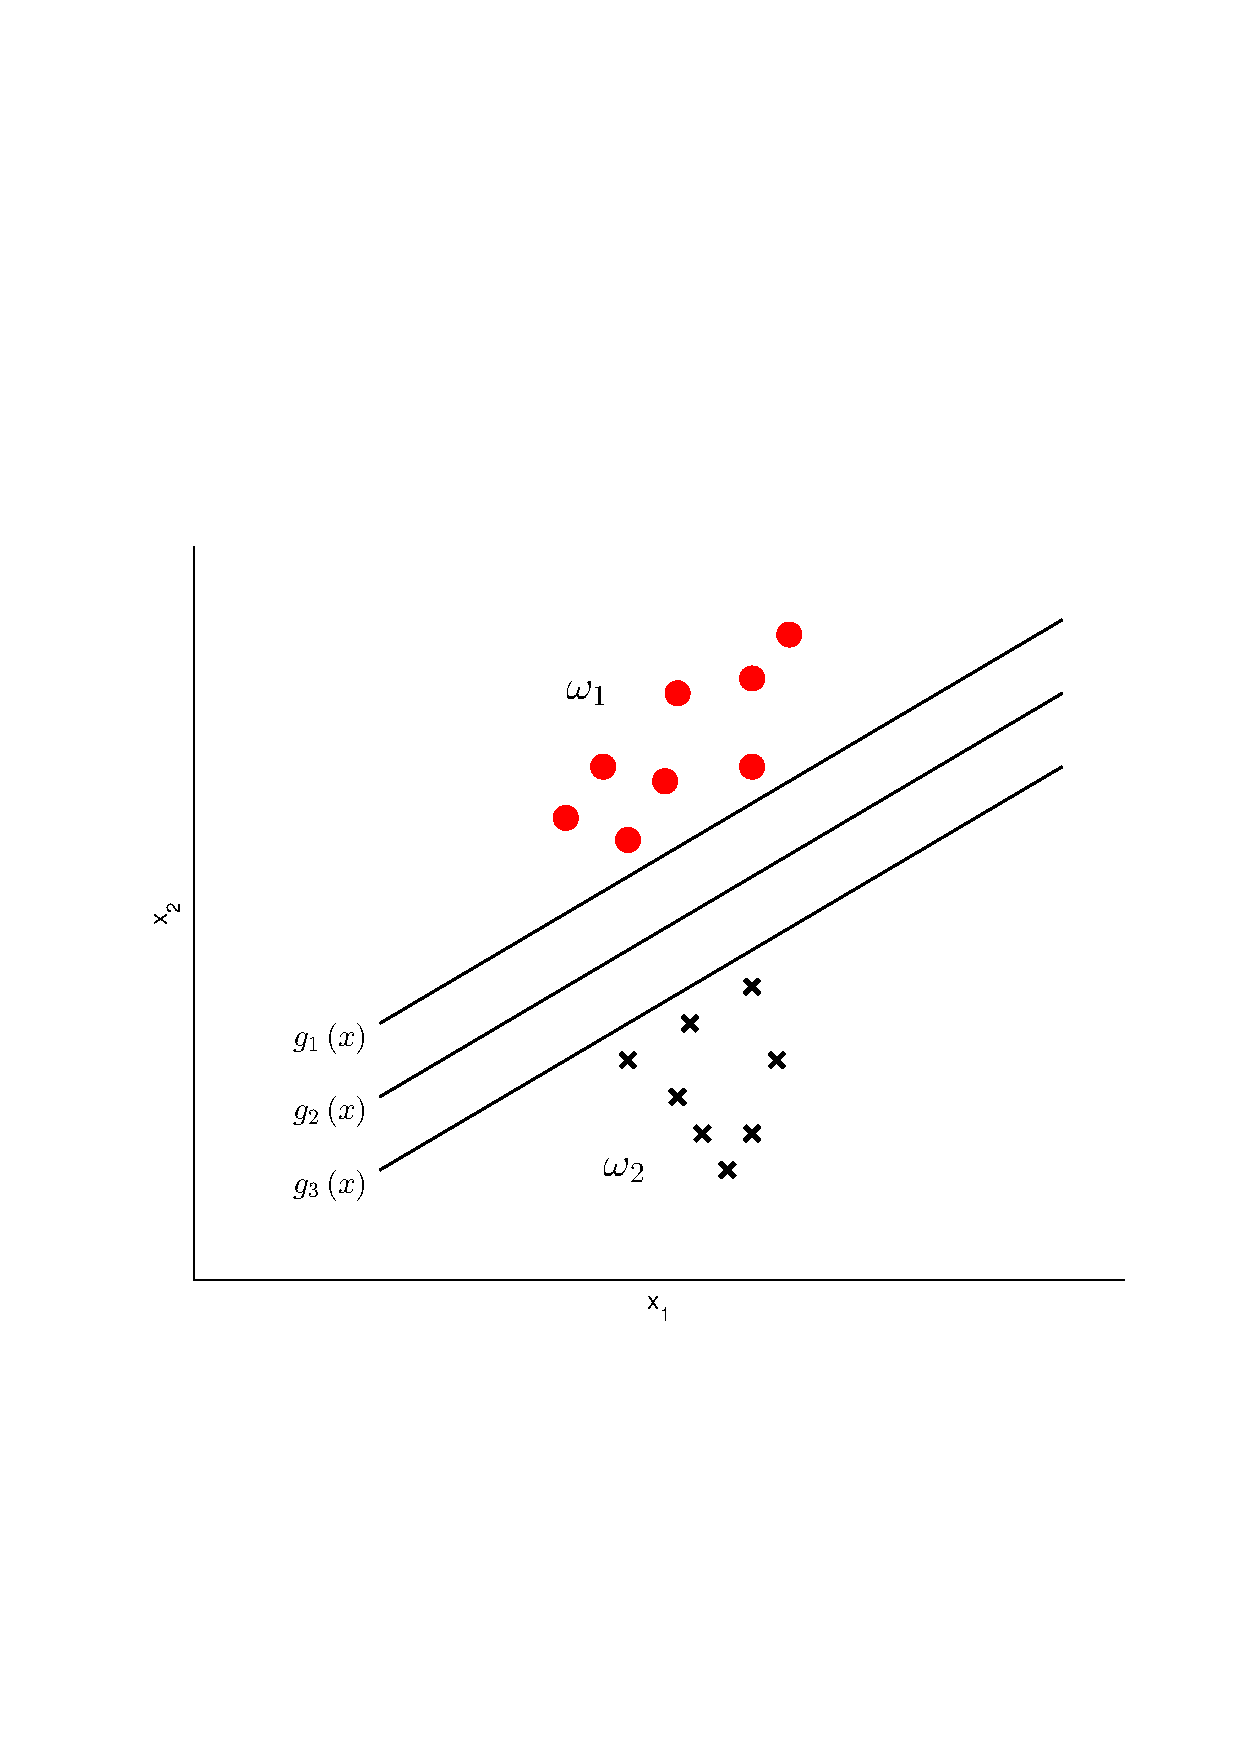
\includegraphics[width = 0.5\textwidth, trim = 3cm 7.5cm 2cm 9cm]{./Img/Prednaska08/SVM/SVM01.pdf}
	\caption{Příklad lineárně separovatelných tříd třemi možnými nadrovinami.}
	\label{fig:SVM01}
\end{figure}}

\par{Obecně je nadrovina definována svým směrem (parametr $\bm{\omega}$) a polohou v prostoru (koeficient $\omega_0$). SVM vedle těchto dvou faktorů zohledňuje i odstup nadroviny od klasifikačních tříd. Jelikož je nežádoucí, aby během určování nadroviny byla některé z tříd zvýhodňována, SVM hledá takový směr $\bm{\omega}$, pro který má nadrovina stejnou vzdálenost k~nejbližším bodům z obou tříd $\omega_1$ a $\omega_2$ (viz Obr. \ref{fig:SVM02}).
\begin{figure}[!ht]
	\centering
	%trim option's parameter order: left bottom right top
	%\fbox{
	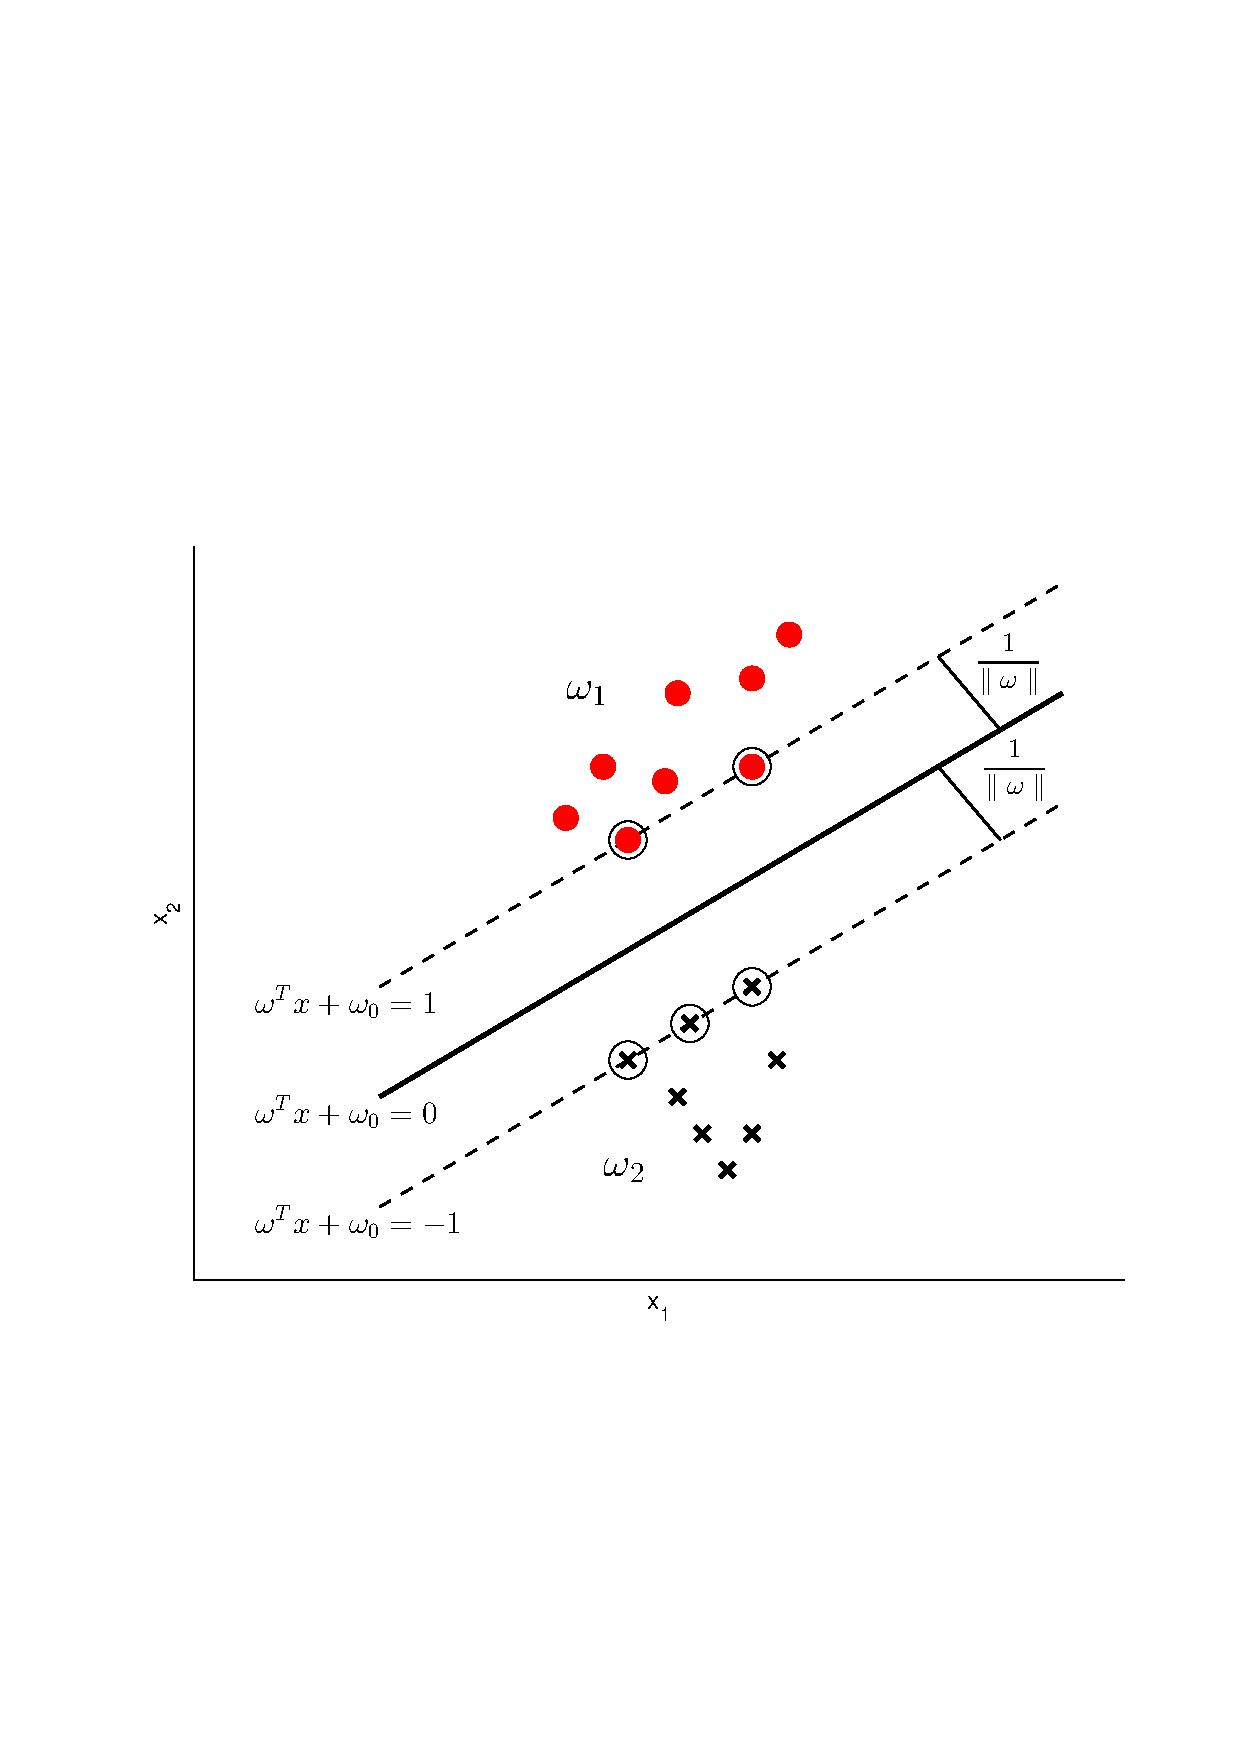
\includegraphics[width = 0.5\textwidth, trim = 3cm 7.5cm 2cm 9cm]{./Img/Prednaska08/SVM/SVM02.pdf}
	\caption{Optimální nadrovina dělící vektory do dvou tříd; kroužkem jsou znázorněny support vectors.}
	\label{fig:SVM02}
\end{figure}}

\par{Vzdálenost mezi bodem a nadrovinou lze vyjádřit pomocí vztahu
\begin{equation}
	{z = \frac{\mid g \left( \bm{x} \right) \mid}{\parallel \bm{\omega} \parallel},}
\end{equation}
kde $\parallel \bm{\omega} \parallel = \sqrt{\bm{\omega}^2}$. Nejblíže položené body (na obr. znázorněny kroužkem) mají vzdálenost od nadroviny rovnu $1$, pokud se nacházejí ve třídě $\omega_1$ a $-1$, náleží-li do třídy $\omega_2$. To vede k závěru, že SVM hledá nadrovinu:
\begin{itemize}
\item mající odstup $\frac{1}{\parallel \bm{\omega} \parallel} + \frac{1}{\parallel \bm{\omega} \parallel} = \frac{2}{\parallel \bm{\omega} \parallel}$.
\item splňující podmínky
\begin{eqnarray}
	\nonumber
	&\bm{\omega}^{\top} \bm{x} + \omega_0 \geq +1,&\textrm{pro}~\forall \bm{x} \in \omega_1,\\
	\nonumber
	&\bm{\omega}^{\top} \bm{x} + \omega_0 \leq -1,&\textrm{pro}~\forall \bm{x} \in \omega_2.
\end{eqnarray}
\end{itemize}
Dále je definován tzv. indikátor třídy $y_i$ ($+1$ pro $\omega_1$ a $-1$ pro $\omega_2$) a cíl metody SVM může být shrnut následovně:
\begin{equation}
	\min J \left( \bm{\omega}, \omega_0 \right) = \frac{1}{2} \parallel \bm{\omega} \parallel^2,
	\label{eq:SVMcostF01}
\end{equation}
za podmínky
\begin{equation}
	y_i \left( \bm{\omega}^{\top} \bm{x}_i + \omega_0 \right) \geq 1,\quad i=1,2,\ldots,N.
	\label{eq:SVMcon01}
\end{equation}
Vektory, pro které platí $y_i \left( \bm{\omega}^{\top} \bm{x}_i + \omega_0 \right) = 1$, jsou označovány jako \textit{support vectors} (viz Obr. \ref{fig:SVM02}).}


\subsubsection*{Matematické řešení}
\par{Z výše uvedených faktů vyplývá, že konstrukce nadroviny, která maximalizuje odstup
od obou klasifikačních tříd, je kvadratickou optimalizační úlohou a její řešení vede na Lagrangeovu funkci, kde $\lambda$ značí Lagrangeův multiplikátor
\begin{equation}
	{\mathcal{L} \left( \bm{\omega},\omega_0,\bm{\lambda} \right)=\frac{1}{2} \bm{\omega}^{\top} \bm{\omega} - \sum_{i=1}^N \lambda_i \left[y_i \left( \bm{\omega}^{\top} \bm{x}_i + \omega_0 \right) - 1 \right],}\label{eq:SVMLagrangian01}
\end{equation}
s podmínkami
\begin{eqnarray}
	\frac{\partial}{\partial \bm{\omega}} \mathcal{L} \left( \bm{\omega},\omega_0,\bm{\lambda} \right)&=&0,\\
	\label{eq:SVMPartial01}
	\frac{\partial}{\partial \omega_0} \mathcal{L} \left( \bm{\omega},\omega_0,\bm{\lambda} \right)&=&0,\\
	\label{eq:SVMPartial02}
	\lambda_i &\geq &0, \quad i=1,2,\ldots,N,\\
	\left[y_i \left( \bm{\omega}^{\top} \bm{x}_i + \omega_0 \right) - 1 \right] &= &0, \quad i=1,2,\ldots,N.
	\label{eq:SVMomegaCon01}
\end{eqnarray}
Kombinací rovnice \ref{eq:SVMLagrangian01} s \ref{eq:SVMPartial01} a \ref{eq:SVMPartial02} je získáno řešení
\begin{eqnarray}
	&\bm{\omega} &= \sum_{i=1}^N \lambda_i y_i \bm{x}_i,\\
	&0 &= \sum_{i=1}^N \lambda_i y_i.
\end{eqnarray}}

\par{Takto zkonstruovaná nadrovina se označuje za nadrovinu optimální. Optimalizační úloha definovaná předpisy \ref{eq:SVMcostF01} a \ref{eq:SVMcon01} patří mezi úlohy konvexního programování a jako takovou ji lze řešit pomocí Lagrangeovy duality
\begin{equation}
	\max \mathcal{L} \left( \bm{\omega},\omega_0,\bm{\lambda} \right),
	\label{eq:SVML01}
\end{equation}
za podmínek
\begin{equation}
	\bm{\omega} = \sum_{i=1}^N \lambda_i y_i \bm{x}_i, \quad \sum_{i=1}^N \lambda_i y_i = 0, \quad  \lambda_i \geq 0, \quad i=1,2,\ldots,N.
	\label{eq:SVMomega01}
\end{equation}
Dosazením rovnic \ref{eq:SVMomega01} do \ref{eq:SVML01} je získána optimalizační úloha ekvivalentní k úloze popsané předpisy \ref{eq:SVMcostF01} a \ref{eq:SVMcon01}
\begin{equation}
	\max_{\lambda} \left( \sum_{i=1}^N \lambda_i - \frac{1}{2} \sum_{i,j} \lambda_i \lambda_j y_i y_j \bm{x}_i^{\top} \bm{x}_j \right),
	\label{eq:SVMmax01}
\end{equation}
s podmínkou
\begin{equation}
	\sum_{i=1}^N \lambda_i y_i = 0, \quad \lambda_i \geq 0, \quad i=1,2,\ldots,N.
\end{equation}
Maximalizováním výrazu \ref{eq:SVMmax01} jsou vypočteny optimální Lagrangeovy multiplikátory a~optimální nadrovina je získána jejich dosazením do rovnice \ref{eq:SVMomega01}. Koeficient $\omega_0$ je vypočten z~podmínky \ref{eq:SVMomegaCon01}.}


\subsubsection*{Nelineárně separovatelná množina}
\par{Jestliže prvky trénovací množiny $X$ nelze lineárně oddělit, nemůžu být výše zmíněný postup konstrukce dělící nadroviny použit. Případ neoddělitelné množiny je zobrazen na obr. Jakýkoli pokus o vykreslení pásu rozdělujícího vektory do dvou tříd skončí neúspěchem. Vždy se totiž uvnitř takového pásu budou vyskytovat vektory trénovací množiny.
\begin{figure}[!ht]
	\centering
	%trim option's parameter order: left bottom right top
	%\fbox{
	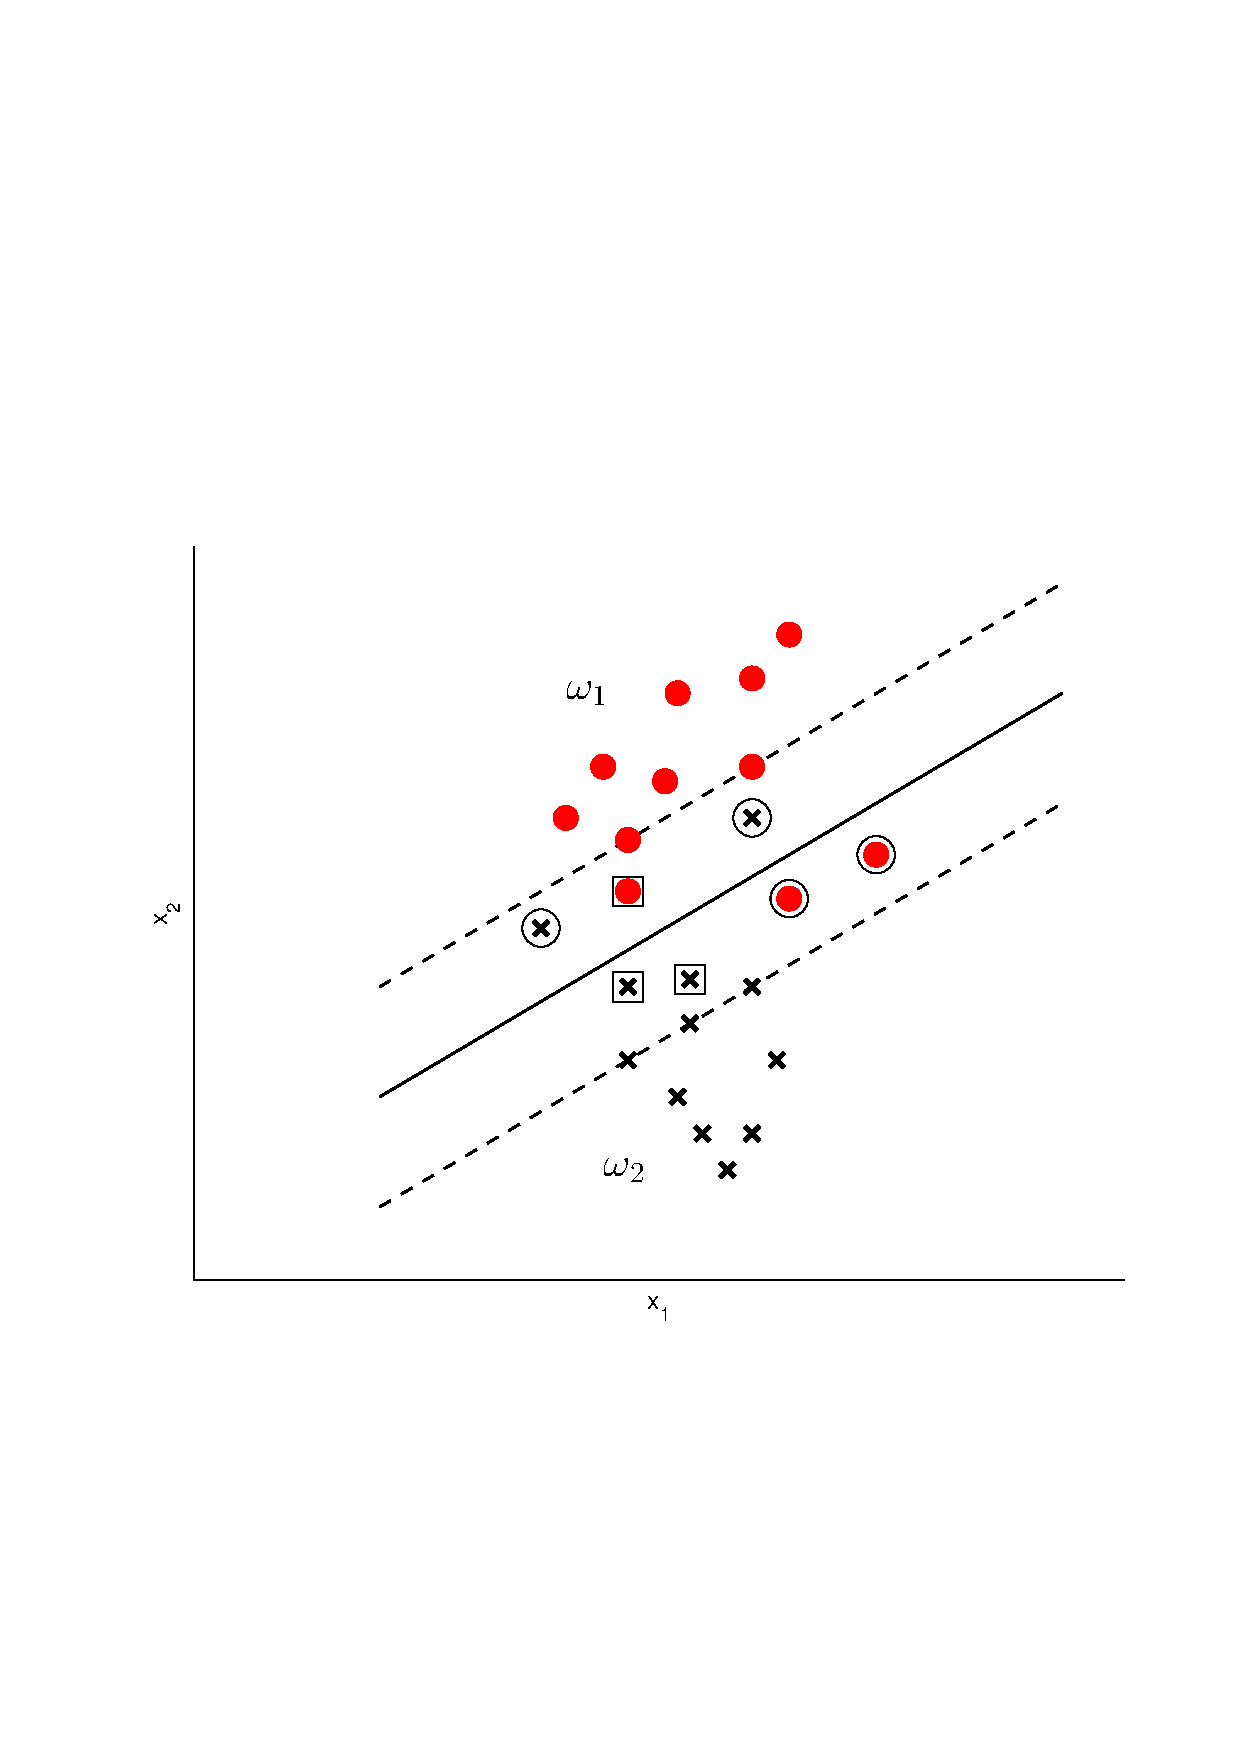
\includegraphics[width = 0.5\textwidth, trim = 3cm 7.5cm 2cm 9cm]{./Img/Prednaska08/SVM/SVM03.pdf}
	\caption{Příklad lineárně neseparovatelné množiny.}
	\label{fig:SVM03}
\end{figure}}

\par{Šířka dělícího pásu je definovaná vzdáleností dvou paralelních nadrovin s předpisem
\begin{equation}
	{\bm{\omega}^{\top} \bm{x} + \omega_0 \pm 1}
\end{equation}
vektory $\bm{x}_i$, $\bm{x}_i \in X$, nyní náleží do jedné ze tří kategorií:
\begin{itemize}
\item vektory ležící mimo dělící pás jsou považovány za správně klasifikované a splňují tak podmínku \ref{eq:SVMcon01}.
\item vektory správně klasifikované, které leží uvnitř pásu, splňují nerovnost (na  Obr. \ref{fig:SVM03} znázorněny čtvercem)
\begin{displaymath}
	{0 \leq y_i \left( \bm{\omega}^{\top} \bm{x} + \omega_0 \right) < 1 .}
\end{displaymath}
\item vektory chybně klasifikované, které leží uvnitř pásu, splňují nerovnost (na Obr. \ref{fig:SVM03} znázorněny kroužkem)
\begin{displaymath}
	{y_i \left( \bm{\omega}^{\top} \bm{x} + \omega_0 \right) < 0.}
\end{displaymath}
\end{itemize}
Všechny tři kategorie mohou být popsány podmínkou
\begin{equation}
	{y_i \left( \bm{\omega}^{\top} \bm{x} + \omega_0 \right) \geq 1- \xi_i,}
\end{equation}
kde $\xi_i$ představuje tzv. klouzavou proměnou. Ta dosahuje hodnoty $\xi_i=0$ pro první kategorii, $0 < \xi_i \leq 1$ pro druhou kategorii a $\xi_i>1$ pro třetí kategorii.}

\par{Úkolem klasifikační metody SVM je opět konstrukce nadroviny, s co největším odstupem od obou tříd, a zároveň minimalizovat počet bodů, pro které je $\xi_i>1$. Jde tedy o~úkol minimalizace ztrátové funkce
\begin{equation}
	{J \left( \bm{\omega}, \omega_0, \bm{\xi} \right) = \frac{1}{2} \parallel \bm{\omega} \parallel^2 + C\sum_{i=1}^N I\left( \xi_i \right),}\label{eq:SVMnonlcostF}
\end{equation}
kde $C$ je pozitivní konstanta, $\bm{\xi}$ je vektor parametrů $\xi_i$ a
\begin{equation}
	I\left( \xi_i \right) = \left\{
	\begin{array}{ll}
		{1,\quad\xi_i>0},\\
		{0,\quad\xi_i=0}.
	\end{array}
	\right.
\end{equation}}


\subsubsection*{Matematické řešení}
\par{Optimalizace funkce \ref{eq:SVMnonlcostF} je matematicky velice složitá, jelikož obsahuje nespojitou funkci $I\left( \bullet \right)$. Z tohoto důvodu se SVM zaměřuje na optimalizaci tzv. blízké funkce a jejím cílem se tak stává
\begin{equation}
	\min J \left( \bm{\omega}, \omega_0, \bm{\xi} \right) = \frac{1}{2} \parallel \bm{\omega} \parallel^2 + C\sum_{i=1}^N \xi_i,
\end{equation}
za podmínek
\begin{equation}
	y_i \left( \bm{\omega}^{\top} \bm{x} + \omega_0 \right) \geq 1 - \xi_i, \quad \xi_i \geq 0,\quad i=1,2,\ldots,N.
\end{equation}
Řešení opět vede na Lagrangeovu funkci
\begin{equation}
	{\mathcal{L} \left( \bm{\omega},\omega_0,\bm{\lambda},\bm{\xi},\bm{\mu} \right)=\frac{1}{2} \parallel \bm{\omega} \parallel^2 + C \sum_{i=1}^N \xi_i - \sum_{i=1}^N \mu_i \xi_i - \sum_{i=1}^N \lambda_i \left[y_i \left( \bm{\omega}^{\top} \bm{x}_i + \omega_0 \right) - 1 + \xi_i\right],}
\end{equation}
za podmínek $\frac{\partial\mathcal{L}}{\partial\bm{\omega}}$, $\frac{\partial\mathcal{L}}{\partial\omega_0}$ a $\frac{\partial\mathcal{L}}{\partial\xi_i}$ nebo
\begin{equation}
	\bm{\omega} = \sum_{i=1}^N \lambda_i y_i \bm{x}_i, \quad \sum_{i=1}^N \lambda_i y_i = 0, \quad C-\mu_i-\lambda_i=0
\end{equation}
společně s podmínkami
\begin{equation}
	\lambda_i \left[y_i \left( \bm{\omega}^{\top} \bm{x}_i + \omega_0 \right) - 1 + \xi_i\right]=0, \quad \mu_i\xi_i=0, \quad \mu_i \geq 0, \quad \lambda_i \geq 0, \quad i=1,2,\ldots,N.
\end{equation}
Použitím Lagrangeovy duality je úkolem SVM
\begin{equation}
	\max \mathcal{L} \left( \bm{\omega},\omega_0,\bm{\lambda},\bm{\xi},\bm{\mu} \right),
	\label{eq:SVMnonlL}
\end{equation}
za podmínek
\begin{equation}
	\bm{\omega} = \sum_{i=1}^N \lambda_i y_i \bm{x}_i, \quad \sum_{i=1}^N \lambda_i y_i = 0, \quad C - \mu_i-\lambda_i=0, \quad \mu_i \geq 0, \quad \lambda_i \geq 0, \quad i=1,2,\ldots,N.
	\label{eq:SVMnonlcon}
\end{equation}
Po dosazení výrazů \ref{eq:SVMnonlcon} do \ref{eq:SVMnonlL} je získána ekvivalentní optimalizační úloha
\begin{equation}
	\max_{\lambda} \left( \sum_{i=1}^N \lambda_i - \frac{1}{2} \sum_{i,j} \lambda_i \lambda_j y_i y_j \bm{x}_i^{\top} \bm{x}_j \right),
\end{equation}
s podmínkou
\begin{equation}
	\sum_{i=1}^N \lambda_i y_i = 0, \quad 0 \leq \lambda_i \leq C, \quad i=1,2,\ldots,N,
\end{equation}
jejímž řešením jsou vypočteny Lagrangeovy multiplikátory. Ty vedou k získání nadroviny, která má maximální možný odstup od obou tříd a zároveň minimalizuje počet vektorů,
pro něž je $\xi_i>0$.}
\newpage






















%-------SVM-KERNEL-TRICK--------------------------------------------------------------------------
%-PETR-ZIMMERMANN-
\section{SVM - Kernel trick}
\label{sec:07_SVM_Kernel_Trick}
\par{Doposud bylo cílem metody SVM lineárně rozdělit trénovací množinu $X$ do dvou tříd $\omega_1$ a $\omega_2$. Mnohdy je ale takový postup řešení neefektivní a vhodnější by bylo v prostoru trénovací množiny zkonstruovat hranici s nelineárním popisem. Za tímto účelem se využívá tzv. \textit{Kernel Trick}, kdy dochází k namapování vstupní množiny $X$ do prostoru vyšší dimenze, v kterém je ji možné lineárně rozdělit (viz Obr. \ref{fig:KT01}).
\begin{figure}[!ht]
	\centering
	%trim option's parameter order: left bottom right top
	%\fbox{
	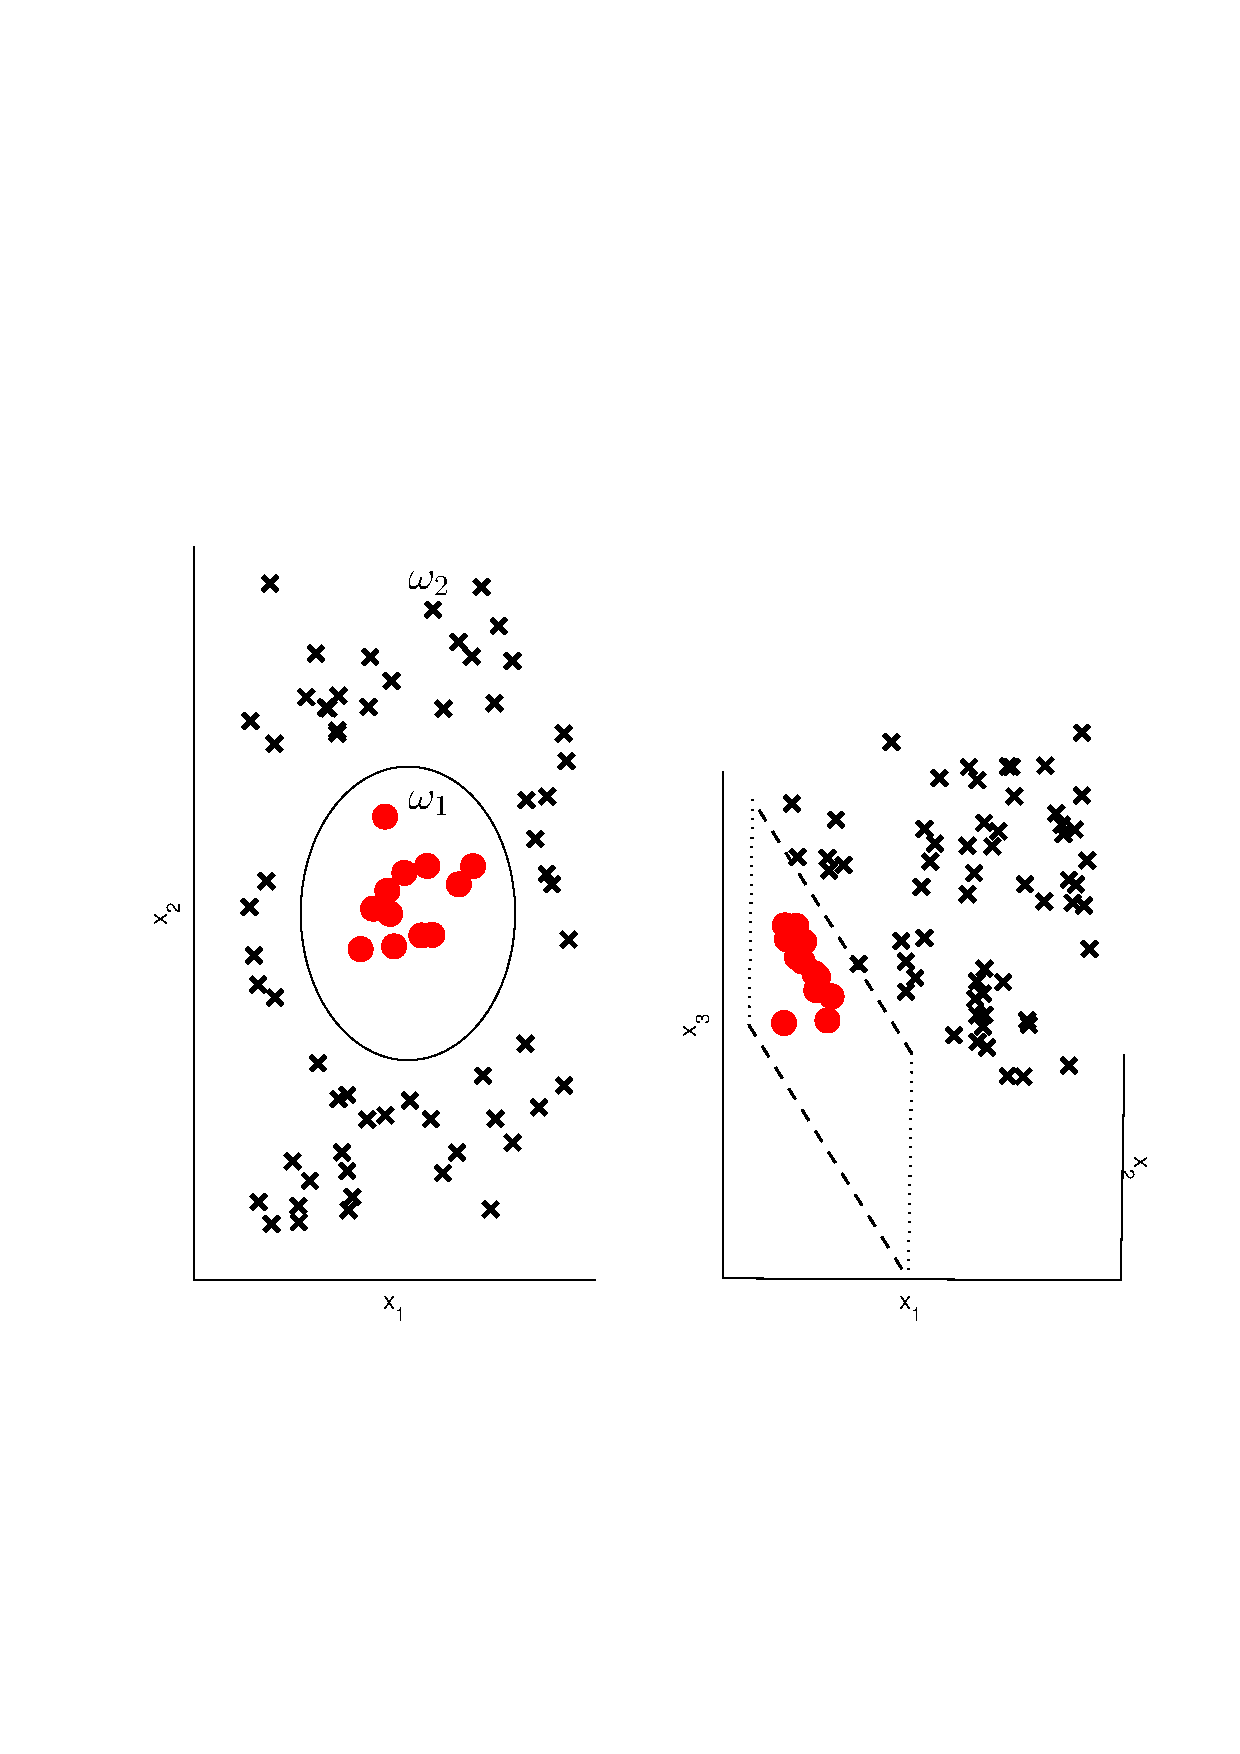
\includegraphics[width = 0.6\textwidth, trim = 3cm 7.5cm 2cm 9cm]{./Img/Prednaska08/SVM/KT01.pdf}
	\caption{Příklad namapování nelineárně separovatelné množiny z prostoru $\mathcal{R}^2$ do prostoru $\mathcal{R}^3$, kde lze množinu lineárně rozdělit.}
	\label{fig:KT01}
\end{figure}}

\par{V rovnici \ref{eq:SVMmax01} je jádro (ang. \textit{kernel}) popsáno vztahem $\bm{x}_i^{\top} \bm{x}_j$ a představuje míru podobnosti mezi $i$-tým a $j$-tým vektorem. Tato míra je označována jako skalární součin (ang. \textit{inner product}). Předpis jádra metody SVM tedy vypadá následovně:
\begin{equation}
	{K\left( \bm{x}_i, \bm{x}_j  \right)= \bm{x}_i^{\top} \bm{x}_j}.
\end{equation} 
Po dosazení předpisu jádra zpět do rovnice \ref{eq:SVMmax01} se cílem metody SVM stává:

\begin{equation}
	{\max_{\lambda} \left( \sum_{i=1}^N \lambda_i - \frac{1}{2} \sum_{i,j} \lambda_i \lambda_j y_i y_j K\left( \bm{x}_i, \bm{x}_j  \right) \right),}
\end{equation}
s podmínkou
\begin{equation}
	\sum_{i=1}^N \lambda_i y_i = 0, \quad \lambda_i \geq 0, \quad i=1,2,\ldots,N.
\end{equation}}

\par{Vhodnou volbou jádra metody SVM lze docílit namapování trénovacích vektorů do prostoru, ve kterém jsou následně aplikovány principy hledání klasifikační nadroviny, jež má maximální možný odstup od nově namapovaných tříd $\omega_1$ a $\omega_2$. Jinými slovy, pomocí \textit{Kernel Trick} je možné metodu SVM, která je metodou lineární, transformovat v metodu nelineární (nelineární klasifikátor). Nejčastěji využívaná nelineární jádra jsou uvedena v~tabulce~\ref{tab:SVMkernels}.
\begin{table}[!ht]
	\centering
	\begin{tabular}{|c|c|c|}
		\hline
		{Typ jádra} & {Předpis} & {Poznámka}\\
		\hline
		\hline		
		{Polynomiální jádro} & {$K\left( \bm{x}_i, \bm{x}_j  \right)=\left( \bm{x}_i \bm{x}_j+\theta \right) ^d$} & {Parametr $d$ a práh $\theta$}\\	
		{} & {} & {je volen uživatelem.}\\	
		\hline
		{Sigmoidové jádro} & {$K\left( \bm{x}_i, \bm{x}_j  \right)= tahh \left( \eta \bm{x}_i \bm{x}_j + \theta \right)$} & {Parametr $\eta$ a práh $\theta$}\\
		{} & {} & {je volen uživatelem.}\\
		\hline
		{Gaussovo jádro} & {$K\left( \bm{x}_i, \bm{x}_j  \right)=exp \left( -\frac{1}{2\sigma^2}\parallel \bm{x}_i - \bm{x}_j \parallel ^2 \right)$} & {Parametr $\sigma$ je}\\
		{\textit{Radial Basis Function}} & {} & {volen uživatelem.}\\
		{(RBF)} & {} & {}\\
		\hline
	\end{tabular}
	\caption{Nejčastěji využívaná nelineární jádra pro metodu SVM.}
	\label{tab:SVMkernels}
\end{table}}

\par{Volbu jádra pro \textit{Kernel Trick} nelze zobecnit. Obvykle se jádra iterativně testují a~vybráno je to, které vykáže nejmenší chybu klasifikace. Často se ovšem doporučuje toto testování odstartovat s RBF jádrem.}














\section{Zdroje}
\label{sec:07_References}


\par{$\left[1\right]$	G. Rätsch, T. Onoda K-R. Müller. \uv{Soft Margins for AdaBoost}, \textit{Machine Learning}, 1-35, August 1998 \newline
$\left[2\right]$	P. Viola and M. Jones, \uv{Fast and Robust Classification using Asymmetric AdaBoost and a Detector Cascade.} Mitsubishi Electric Research Lab, Cambridge, MA. 2001 \newline
$\left[3\right]$	Cortes C., Vapnik V., \uv{Support Vector Networks}, \textit{Machine Learning}, vol. 20, pp. 273-297, 1995.\newline
$\left[4\right]$	Theodoridis S., Koutroubas K., \textit{Pattern Recognition}, Elsevier Inc., 2008.}



























\end{document}

